%--------------------------------------------------------------------------------------%--------------------------------------------------------------------------------------
%
%  Global settings, dont change it! (excapt additional \usepackage commands)
%  Always use PDFLatex!
%
%--------------------------------------------------------------------------------------%--------------------------------------------------------------------------------------
\documentclass[a4paper, 12pt, oneside, openany, BCOR1cm,toc=chapterentrywithdots]{scrbook}

\usepackage{graphicx}           % use for pdfLatex
\usepackage{makeidx} % f\"{u}r Benutzung des Befehls \printindex
\usepackage[colorlinks=false]{hyperref}
\usepackage{tocbibind}
\usepackage{blindtext}
\usepackage{subfigure}
\usepackage{acronym}
\usepackage[table]{xcolor}
\usepackage{pifont}
\usepackage{booktabs}
\newcommand{\cmark}{\textcolor{green!45!black}{\ding{51}}}
\newcommand{\xmark}{\textcolor{red!60!black}{\ding{55}}}

% --------------------------------------------------------------
% Standard table style: dark green header row with white bold
% text, zebra-striped body, no vertical rules. Use \thw{...} for
% each header cell and \rowcolors{2}{green!5}{white} right before
% \begin{tabular} on every table for a consistent look.
% --------------------------------------------------------------
\newcommand{\thw}[1]{\textcolor{white}{\textbf{#1}}}

\hypersetup{%
bookmarksnumbered=true, hyperindex=true,
%
%Im Acrobat Reader Subtitel 1. Ebene anzeigen
bookmarksopen=true, bookmarksopenlevel=1,
%
pdfborder=0 0 0 % Keine Box um die Links!
}

% --------------------------------------------------------------
% Force Tables and List to be added in Table of Content
% --------------------------------------------------------------

\renewcommand*{\tableofcontents}{%
  	\begingroup
  	\tocsection
  	\tocfile{\contentsname}{toc}
  	\endgroup
}
\renewcommand*{\listoffigures}{%
  	\begingroup
  	\tocsection
  	\tocfile{\listfigurename}{lof}
  	\endgroup
}
\renewcommand{\listoftables}{
	\begingroup
	\tocsection
	\tocfile{\listtablename}{lot}
	\endgroup
}
\begin{document}

%--------------------------------------------------------------------------------------%--------------------------------------------------------------------------------------
%
%  Here starts the userspace !
%
%--------------------------------------------------------------------------------------%--------------------------------------------------------------------------------------

%--------titlepage
\begin{titlepage}

{
    \begin{center}
        \raisebox{-1ex}{
\includegraphics[scale=1.5]{TU_Chemnitz_positiv_gruen.pdf}}\\
    \end{center}
    \vspace{0.3cm}
}

\begin{center}

\LARGE{\textbf{Recommendation System for ASPICE (SWE1-SWE6) Process Assessment}}\\
\vspace{0.7cm}

\Large{\textbf{Master Thesis}}\\
\vspace{0.7cm}
Submitted in Fulfilment of the\\
Requirements for the Academic Degree\\
M.Sc. Automotive Software Engineering\\
\vspace{0.5cm}
Dept. of Computer Science\\
Chair of Computer Engineering
\end{center}
\vspace{1.0cm}
Submitted by: Faizan Ahmed\\
Student ID: 763411\\
Date: 17.09.2026\\
\vspace{0.3cm}\\
Supervising tutors:  \\
Prof. Dr. Wolfram Hardt (TU Chemnitz) \\
Dr. Dimitrios Datsogiannis (BMW)\\

\end{titlepage}

%---------------------------------------------------------
% Acknowledgments
%---------------------------------------------------------

\addchap*{Acknowledgments}

I would like to express my deepest gratitude to my supervisors, Prof. Dr. Dr.
h. c. Wolfram Hardt, Dr. Dimitrios Datsogiannis and Sophie Jacobi, for their continuous guidance, insightful feedback, and unwavering
support throughout this research. Their expertise, encouragement, and constructive
criticism have been invaluable in shaping this work and helping me grow as a
researcher.

I am also profoundly grateful to my colleagues and friends especially Kaleem Ullah, whose encouragement,
discussions, and companionship have made this journey both inspiring and enjoyable.
Their support, laughter, and shared experiences have enriched not only my
research but also my personal growth during these years.

I would like to extend my gratitude to every person I have crossed paths with,
whether directly or indirectly. Each interaction, experience, and shared moment has
contributed to shaping me into the person I am today. Your influence, in small or
large ways, has left an enduring impact that I carry with me.

Finally, I wish to thank my family for their unconditional love, patience, and
unwavering belief in me. Their constant support has been my foundation, giving
me the strength and motivation to overcome challenges and pursue my goals. I am
deeply grateful for their encouragement, understanding, and the sacrifices they have
made to allow me to focus on my studies. Their guidance, wisdom, and kindness have
shaped not only my academic journey but also the person I am today. The values
they have instilled in me, their steadfast presence in both joyous and difficult times,
and their endless love have been a source of inspiration throughout this journey. I
am profoundly thankful to have them by my side, and I dedicate the completion of
this thesis to their enduring support.

%---------------------------------------------------------
% Abstract
%---------------------------------------------------------

\addchap*{Abstract}

Automotive Software Process Improvement and Capability dEtermination (ASPICE) assessment provides automotive software suppliers with a capability
rating, but at audit time only; there is no mechanism to determine whether a process is still
being followed correctly between audits. A weakness introduced right after an audit may go
undetected, and become much more costly to fix, by the time it is eventually discovered. Prior
work has proposed a solution to this problem using a contextual multi-armed bandit (CMAB) that
dynamically selects assessment questions rather than relying on a fixed questionnaire, but this
has not yet been evaluated in a real-world deployment.

In this research, a real, deployed system for continuous ASPICE assessment of the Software
Engineering process group (SWE.1 to SWE.6) at capability levels L1 to L3 is developed and
evaluated. A 60-question bank is derived directly from the ASPICE base practices and targeted at
specific stakeholder roles, with each question's answer options weighted from 0 (practice fully
in place) to 5 (practice effectively absent). Rather than asking every question in the bank, a
CMAB-based recommendation engine selects a small number of questions for each session, chosen
according to the stakeholder's role and the session's progress so far. A rule-based classifier
then scores and ranks process weaknesses automatically, without needing a labelled training set
or a human assessor's judgement. These weaknesses are made visible on a results dashboard as
soon as a session is completed. The system is implemented end to end with FastAPI, React, and
PostgreSQL.

Unlike the prior simulation-based work, this research evaluates the system in a live pilot
rather than in simulation: the pilot was self-administered by the author across all seven
stakeholder roles, with seventeen sessions started and fifteen completed. The processes the
recommendation engine asks about most often are the same ones the classifier independently
scores as the weakest across the pilot, an indication that the mechanism behaves sensibly on
real data, not only on simulated data. A single session's result can also differ sharply from
the overall result for that process, underscoring the need for early, per-session visibility.
The pilot reflects real usage, but is limited in scale and self-administered rather than run
with independent participants, and the weights in the question bank have not yet been checked
by a certified assessor; both points are stated explicitly as limitations. Overall, the results
show that adaptive, continuous ASPICE assessment is not only a viable idea but a working one.
\\\\
\textbf{Keywords: ASPICE, Recommender Systems, Contextual Multi-Armed Bandit, LinUCB, Process Assessment}

%---------------------------------------------------------
% Table of Contents, List of figures, List of Tables
%---------------------------------------------------------

\tableofcontents
\listoffigures
\listoftables

%---------------------------------------------------------
% List of Abbreviations
%---------------------------------------------------------
\twocolumn
\addchap{List of Abbreviations}
\begin{acronym}[HTTPS]
 \acro{ASPICE}{Automotive Software Process Improvement and Capability dEtermination}
 \acro{SPICE}{Software Process Improvement and Capability dEtermination}
 \acro{VDA}{Verband der Automobilindustrie (German Association of the Automotive Industry)}
 \acro{OEM}{Original Equipment Manufacturer}
 \acro{PRM}{Process Reference Model}
 \acro{PAM}{Process Assessment Model}
 \acro{BP}{Base Practice}
 \acro{SWE}{Software Engineering (process group)}
 \acro{MAB}{Multi-Armed Bandit}
 \acro{CMAB}{Contextual Multi-Armed Bandit}
 \acro{UCB}{Upper Confidence Bound}
 \acro{LinUCB}{Linear Upper Confidence Bound}
 \acro{RL}{Reinforcement Learning}
 \acro{ER}{Entity-Relationship}
 \acro{CRUD}{Create, Read, Update, Delete}
 \acro{ORM}{Object-Relational Mapping}
 \acro{API}{Application Programming Interface}
 \acro{REST}{Representational State Transfer}
 \acro{JWT}{JSON Web Token}
 \acro{JSON}{JavaScript Object Notation}
 \acro{SQL}{Structured Query Language}
 \acro{DB}{Database}
 \acro{UI}{User Interface}
 \acro{UX}{User Experience}
 \acro{GUI}{Graphical User Interface}
 \acro{HTTP}{Hypertext Transfer Protocol}
 \acro{HTTPS}{Hypertext Transfer Protocol Secure}
 \acro{TLS}{Transport Layer Security}
\end{acronym}

\onecolumn
%---------------------------------------------------------
% Here starts the real work
%---------------------------------------------------------

\chapter{Introduction}
\label{chap:introduction}
% \input{src/introduction}

In this chapter, the context and main problem of this research are outlined and the main
objectives are defined. It starts with the problem statement and the motivation, emphasizing the
need for a continuous assessment of the process in automotive software development. It then
introduces the research questions, contribution of this work, scope of the work and concludes by
providing an overview of the thesis structure.

\section{Problem Statement}

Automotive Software Process Improvement and Capability dEtermination (ASPICE) is an automotive
process assessment model developed by the automotive OEMs and suppliers to assess the
implementation of software process at a supplier~\cite{vdaqmc2023pam}. Does not evaluate
software. Instead it concentrates on the process: Proper analysis of requirements, consistency of
architecture and detailed design with requirements, and software verifiability. In the Software
Engineering process group -- SWE.1 to SWE.6 -- this involves looking at each stage of the
process, from analysis of the requirements through to the final verification of the software.

This evaluation is done on a structured manner in practice, which is known as an audit. At
specific points in the project, an assessment team led by a certified assessor comes in and
evaluates available evidence and assigns a score to each process on a predetermined scale of NOT achieved to FULLY
achieved~\cite{vdaqmc2023pam,murphy_aspice_0to60}. This method is good for evaluating process
capability at a given time, but it leaves gaps that this thesis tackles: it gives no visibility
into what happens between audits, it relies on a long, fixed questionnaire that is worked through
in full regardless of what is actually relevant to a given session, and it depends on a human
assessor's judgement to turn the evidence collected into a weakness rating.

The most immediate of these is the gap between audits. After a project has been evaluated, there is no
ongoing method to check if the project process is continuing to be implemented properly. A
weakness can be introduced just after an audit, like a poorly thought out requirement or a design
decision that is not checked at any point after it's made, and go unnoticed for months. It might
only be seen at the next audit or even at a later audit when it is presented as a
defect~\cite{datsogiannis2024early}. At that time, solving the problem might be quite expensive,
compared to if it had been solved earlier~\cite{schauffele2016automotive,jiang2013earlylifecycle}.
Even when applied exactly as intended, ASPICE cannot close this gap: by design, it produces a
rating only at the time of the audit and gives a development team no signal to act on in
between.

This thesis begins by exploring this gap -- can the SWE.1 -- SWE.6 base practices be translated to
something that stakeholders can refer to continuously as part of their daily development
activities, not just when an assessor is present?

\section{Motivation}

This thesis is motivated by a problem faced in modern car software development. Car software is
becoming more and more complex, and each new generation must remain compatible with in-vehicle
systems, cloud services, and other vehicles~\cite{zhang2021canbus,furst2010challenges}.
The more complex it becomes the more challenging it is to identify weaknesses in the process and
to remediate them, if they are discovered at the end of the process. The importance of regular and
effective process assessment is growing, as a result of this.

ASPICE has established a good framework for Software Development Process
Assessment. In the past, however, the assessment is predominantly carried out by regularly
scheduled and structured audits. While not all questions are equally useful in all situations, in
most cases stakeholders are asked a large number of pre-determined questions. There might be a few
questions that don't give you much information, and another question, at just the right moment,
could give you a clue to a weakness. This raises an important question: can fewer, more relevant
questions achieve the same insight?

This idea is further supported by research on reinforcement learning (RL) recommender systems, which
have been shown to be able to adapt to a specific situation by learning to choose more useful
questions rather than strictly playing a pre-defined sequence~\cite{datsogiannis2024early}. This
is the same principle that can be used for an ASPICE assessment. The utility of a question may
vary each time it is asked, depending on what has already been addressed, the process areas
that are perceived as being not strong enough, the capability being explored, and the stakeholder
who is answering the question. A contextual multi-armed bandit (CMAB) is thus an appropriate
solution as it can leverage on this evolving context to determine the next question to ask.

The selection of questions based on ASPICE has been studied before, in a CMAB
setting~\cite{datsogiannis2024early} and comparing each of the bandit algorithms in simulated
settings~\cite{datsogiannis2025recommender}. One thing remains though -- getting from a
successful concept that has been simulated to an actual system that has been tested via real
assessment data. This is the primary reason behind this thesis.

The thesis thus creates a web-based program which is able to adaptively pick questions from the
SWE.1--SWE.6 process group according to the information it has at an assessment session. The
answers then are used to pinpoint and categorize potential process weaknesses. It is not intended
to supplant the expertise of the individual or ASPICE principles. Rather, the intent is to focus
the assessment process by suggesting the right question and the right time in the system.

In the end, the motivation for this research is for the possibility to reduce reliance on long and
static questionnaires in process assessment, and make it more responsive to the situation being
assessed. This thesis seeks to demonstrate that adaptive question selection can make ASPICE
assessment not only practical to use, but also continuous over time, as it is implemented as a
working web application and tested using actual audit sessions, instead of simulated data.

\section{Research Questions}

The thesis has four research questions:

\begin{itemize}
  \item \textbf{RQ1.} How can the base practices of ASPICE SWE.1--SWE.6 be systematically
  converted into a structured, weighted question bank of auditor-style questions, aligned with
  SWE processes and stakeholder roles?
  \item \textbf{RQ2.} How can a web-based recommendation system narrow the question bank down
  to a few questions that are well-targeted in the evaluation cycle?
  \item \textbf{RQ3.} How do the stakeholder answers get automatically classified to a process
  weakness rating for each of the SWE processes without a human assessor's judgement?
  \item \textbf{RQ4.} How can these results be communicated in such a way that process
  deficiencies (and their evolution from version to version of the software) can be identified
  early, and not just at the next scheduled ASPICE audit?
\end{itemize}

\section{Contributions}

The following are the contributions aligned to the above research questions:

\begin{itemize}
  \item \textbf{RQ1.} A well-organised question bank covering the ASPICE SWE.1 -- SWE.6, with
  each question linking to a specific base practice, and stakeholder roles and weighted answers
  assigned.
  \item \textbf{RQ2.} A CMAB-based recommendation engine using the LinUCB algorithm, that
  recommends a few well-targeted questions per session to a user, based on a session-state
  context that includes what the stakeholder has done, how far he has progressed and what the
  process and capability level of the session has accomplished to date.
  \item \textbf{RQ3.} A rule based weakness classifier that is able to score each (process,
  capability level) cell assessed, and automatically rank each weakness, without the need of a
  labelled training data set, or human assessor's judgement.
  \item \textbf{RQ4.} Early visibility of weakness classifications for each SWE process and their
  trends over sessions in a results dashboard - instead of having to wait for the next scheduled
  audit.
  \item A full end-to-end web application that integrates the four contributions above using
  FastAPI, React and PostgreSQL for real users.
  \item This is followed by a real evaluation of pilot sessions that are not simulated. This
  thesis gives this evaluation for the scope SWE.1--SWE.6, while both papers from the
  supervisors~\cite{datsogiannis2024early,datsogiannis2025recommender} leave it for future work.
\end{itemize}

\section{Scope and Limitations}

This research deals with one component of ASPICE: the Software Engineering process group,
SWE.1 through SWE.6, and capability levels L1 to L3 (Performed, Managed, Established).
System Engineering, Validation, Management, Supporting, and Process
Improvement are not covered, and neither are capability levels L4 and L5. The higher levels address quantitative process control and organisation-wide
improvement, and rely on information from several projects, over a period of time, and not
information that a stakeholder can provide during one session.

This limited scope introduces two weaknesses that will be highlighted here.

\begin{itemize}
  \item The capability levels L2 and L3 are partially based on the definition and deployment of a
  process in an organization, not just on the execution of the process in a single
  project~\cite{vdaqmc2023pam}. This can only be addressed by one stakeholder in a session, but
  not by an assessor who will have a look at the process assets that the organization actually
  uses.
  \item A panel of independent experts did not validate the weights given to the answer options
  in this thesis. These question weights were inspired by this
  work~\cite{datsogiannis2024early}, and it is left for future work to validate these weights
  here.
\end{itemize}

\section{Structure of the Thesis}

Chapter~\ref{chap:background} presents a brief introduction to the ASPICE, recommender systems
and multi armed bandits, which will be needed to follow the discussion that follows. In
Chapter~\ref{chap:sota} this thesis is compared to the two papers of the supervisors mentioned
above and compared to the use of ASPICE as it is usually done. In Chapter~\ref{chap:architecture},
the design of the system is explained, that is, the database schema, the engine of the CMAB, the
weakness classifier, and the design of the API and frontend. Chapter~\ref{chap:implementation}
explains how this design has been realized. Chapter~\ref{chap:results} explains how the system
was evaluated and presents the results of that evaluation. Finally, Chapter~\ref{chap:conclusion}
is a recap of the research questions and what is still to be done.

\chapter{Background and Fundamentals}
\label{chap:background}
% \input{src/background}

In this chapter, the three major concepts that are the core of this research are introduced: what
is ASPICE, how is it typically performed, what is a recommender system, and what is a
multi-armed bandit. This chapter will introduce you to the core concepts and important terms
behind each of these topics, since Chapter~\ref{chap:architecture} assumes you already know them.

\section{Automotive SPICE (ASPICE)}

The automotive OEMs and suppliers have adopted a process assessment model called ASPICE to
assess the capability of automotive suppliers in software and systems
development~\cite{vdaqmc2023pam}. Does not evaluate the product itself. Rather, it evaluates the
process that is followed to create that product. That is, a supplier is not only judged on the
software's functionality, but also on whether requirements were captured against, designed against,
implemented against, and verified by the software's development process consistently.

\subsection{Process Reference and Assessment Models (PRM/PAM)}

ASPICE is based on two interrelated models. The Processes Reference Model (PRM) outlines the
processes to be assessed against a supplier and the intent and desired results of each process.
The Process Assessment Model (PAM) then provides what is needed to actually assess those
processes: a set of capability levels and indicators, known as base practices and generic
practices, that an assessor looks for as evidence~\cite{vdaqmc2023pam}. These models complement
each other in a 2-D way: a process dimension, determining the process being assessed, and a
capability dimension, determining the capability of the assessed process. The dimension of
capability, which is the one that the ASPICE measurement framework uses, is taken from the
internationally agreed process assessment standard
ISO/IEC~33020~\cite{iso33020_2019,vdaqmc2023pam}. The terms of its core concepts, such as
information item and process attribute are taken from ISO/IEC~33001~\cite{iso33001_2015}.

The total process reference model as kept by the VDA Quality Management Center, who maintains the
ASPICE standard~\cite{vdaqmc_website,vdaqmc2023pam}, is shown in Figure~\ref{fig:aspice-model}.
The processes are segmented into three life-cycle categories and then into process groups with
each process group having a two-letter code.

\begin{figure}[h]
  \centering
  
\includegraphics[width=\textwidth]{src/aspice_model.png}
  \caption{The Automotive SPICE process reference model, with SWE highlighted in red.
  Reproduced from the VDA Quality Management Center~\cite{vdaqmc_website,vdaqmc2023pam}.}
  \label{fig:aspice-model}
\end{figure}

\begin{description}
  \item[Acquisition (ACQ)] The work of an outside contractor.
  \item[Supply (SPL)] Deals with the way in which a product is supplied to a customer.
  \item[System Engineering (SYS)] Brings stakeholder needs from system-level requirements to
  system architecture, integration and verification.
  \item[Software Engineering (SWE)] The software level development flow, from requirements to
  verification, is the process group used in this thesis.
  \item[Hardware Engineering (HWE)] The equivalent development processes for hardware components.
  \item[Machine Learning Engineering (MLE)] Covers requirements, architecture, training and
  testing of machine-learning components.
  \item[Validation (VAL)] Determines if the completed product fulfills the expectations of the
  stakeholders that are experienced in the real world, not just in the written requirements.
  \item[Supporting Process (SUP)] Covers quality assurance, configuration management, problem
  resolution management, change request management, and machine-learning data management.
  \item[Management (MAN)] Is about project management, risk management and measurement.
  \item[Process Improvement (PIM)] Deals with the improvement of processes as time passes.
  \item[Reuse (REU)] Is for managing products that can be used again for various projects.
\end{description}

This is a grouping that will enable a supplier to be evaluated only on the process groups that it
actually develops. This thesis is confined to a single, main life-cycle group: Software
Engineering (SWE).

\subsection{The SWE Process Group: SWE.1--SWE.6}

The Software Engineering process group includes all the software engineering activities from
defining software requirements through verifying the software. It is made up of 6 processes as
described below.

Figure~\ref{fig:v-model} shows the V-model view of the SWE.1--SWE.6
processes~\cite{vmodel_visure}.

\begin{figure}[h]
  \centering
  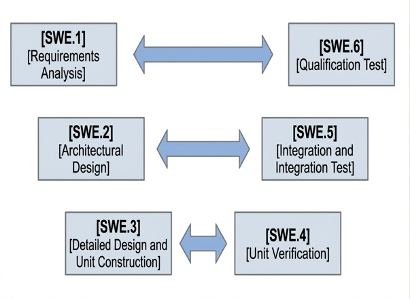
\includegraphics[width=\textwidth]{src/v-model.png}
  \caption{The V-model view of the SWE.1--SWE.6 processes. Adapted from~\cite{vmodel_visure}.}
  \label{fig:v-model}
\end{figure}

\begin{description}
  \item[SWE.1: Software Requirements Analysis] Records the software requirements that are
  extracted from the System Requirements and System Architecture.
  \item[SWE.2: Software Architectural Design] Describes the software architecture, which is
  the division of software into components and the interactions between the components.
  \item[SWE.3: Software Detailed Design and Unit Construction] Specifies each software unit in
  detail and constructs it.
  \item[SWE.4: Software Unit Verification] Verifies that each implemented unit meets its
  detailed design.
  \item[SWE.5: Software Integration and Integration Test] Integrates verified units into
  larger components and the complete software build, and tests if this integration is correct.
  \item[SWE.6: Software Qualification Test] Tests the fully integrated software against the
  original software requirements.
\end{description}

The six processes are grouped around the V-shape as shown in Figure~\ref{fig:v-model}: SWE.1
(requirements) is paired with SWE.6 (software qualification test), SWE.2 (architecture) is
paired with SWE.5 (integration test), and SWE.3 (detailed design) is paired with SWE.4 (unit
verification)~\cite{vdaqmc2023pam}. There are base practices for each process, these are the
specific activities an assessor is looking for. These are the base practices that are directly
used in this thesis as the source material for the question bank described in
Chapter~\ref{chap:implementation}.

\subsection{Capability Levels and Base Practices (L1--L3)}

Processes cannot be just said to be present or not. ASPICE establishes six capability levels (see
Figure~\ref{fig:capability-levels}) and a process can only attain a specific level if it meets
all the levels on its way to the specified level.

\begin{figure}[h]
  \centering
  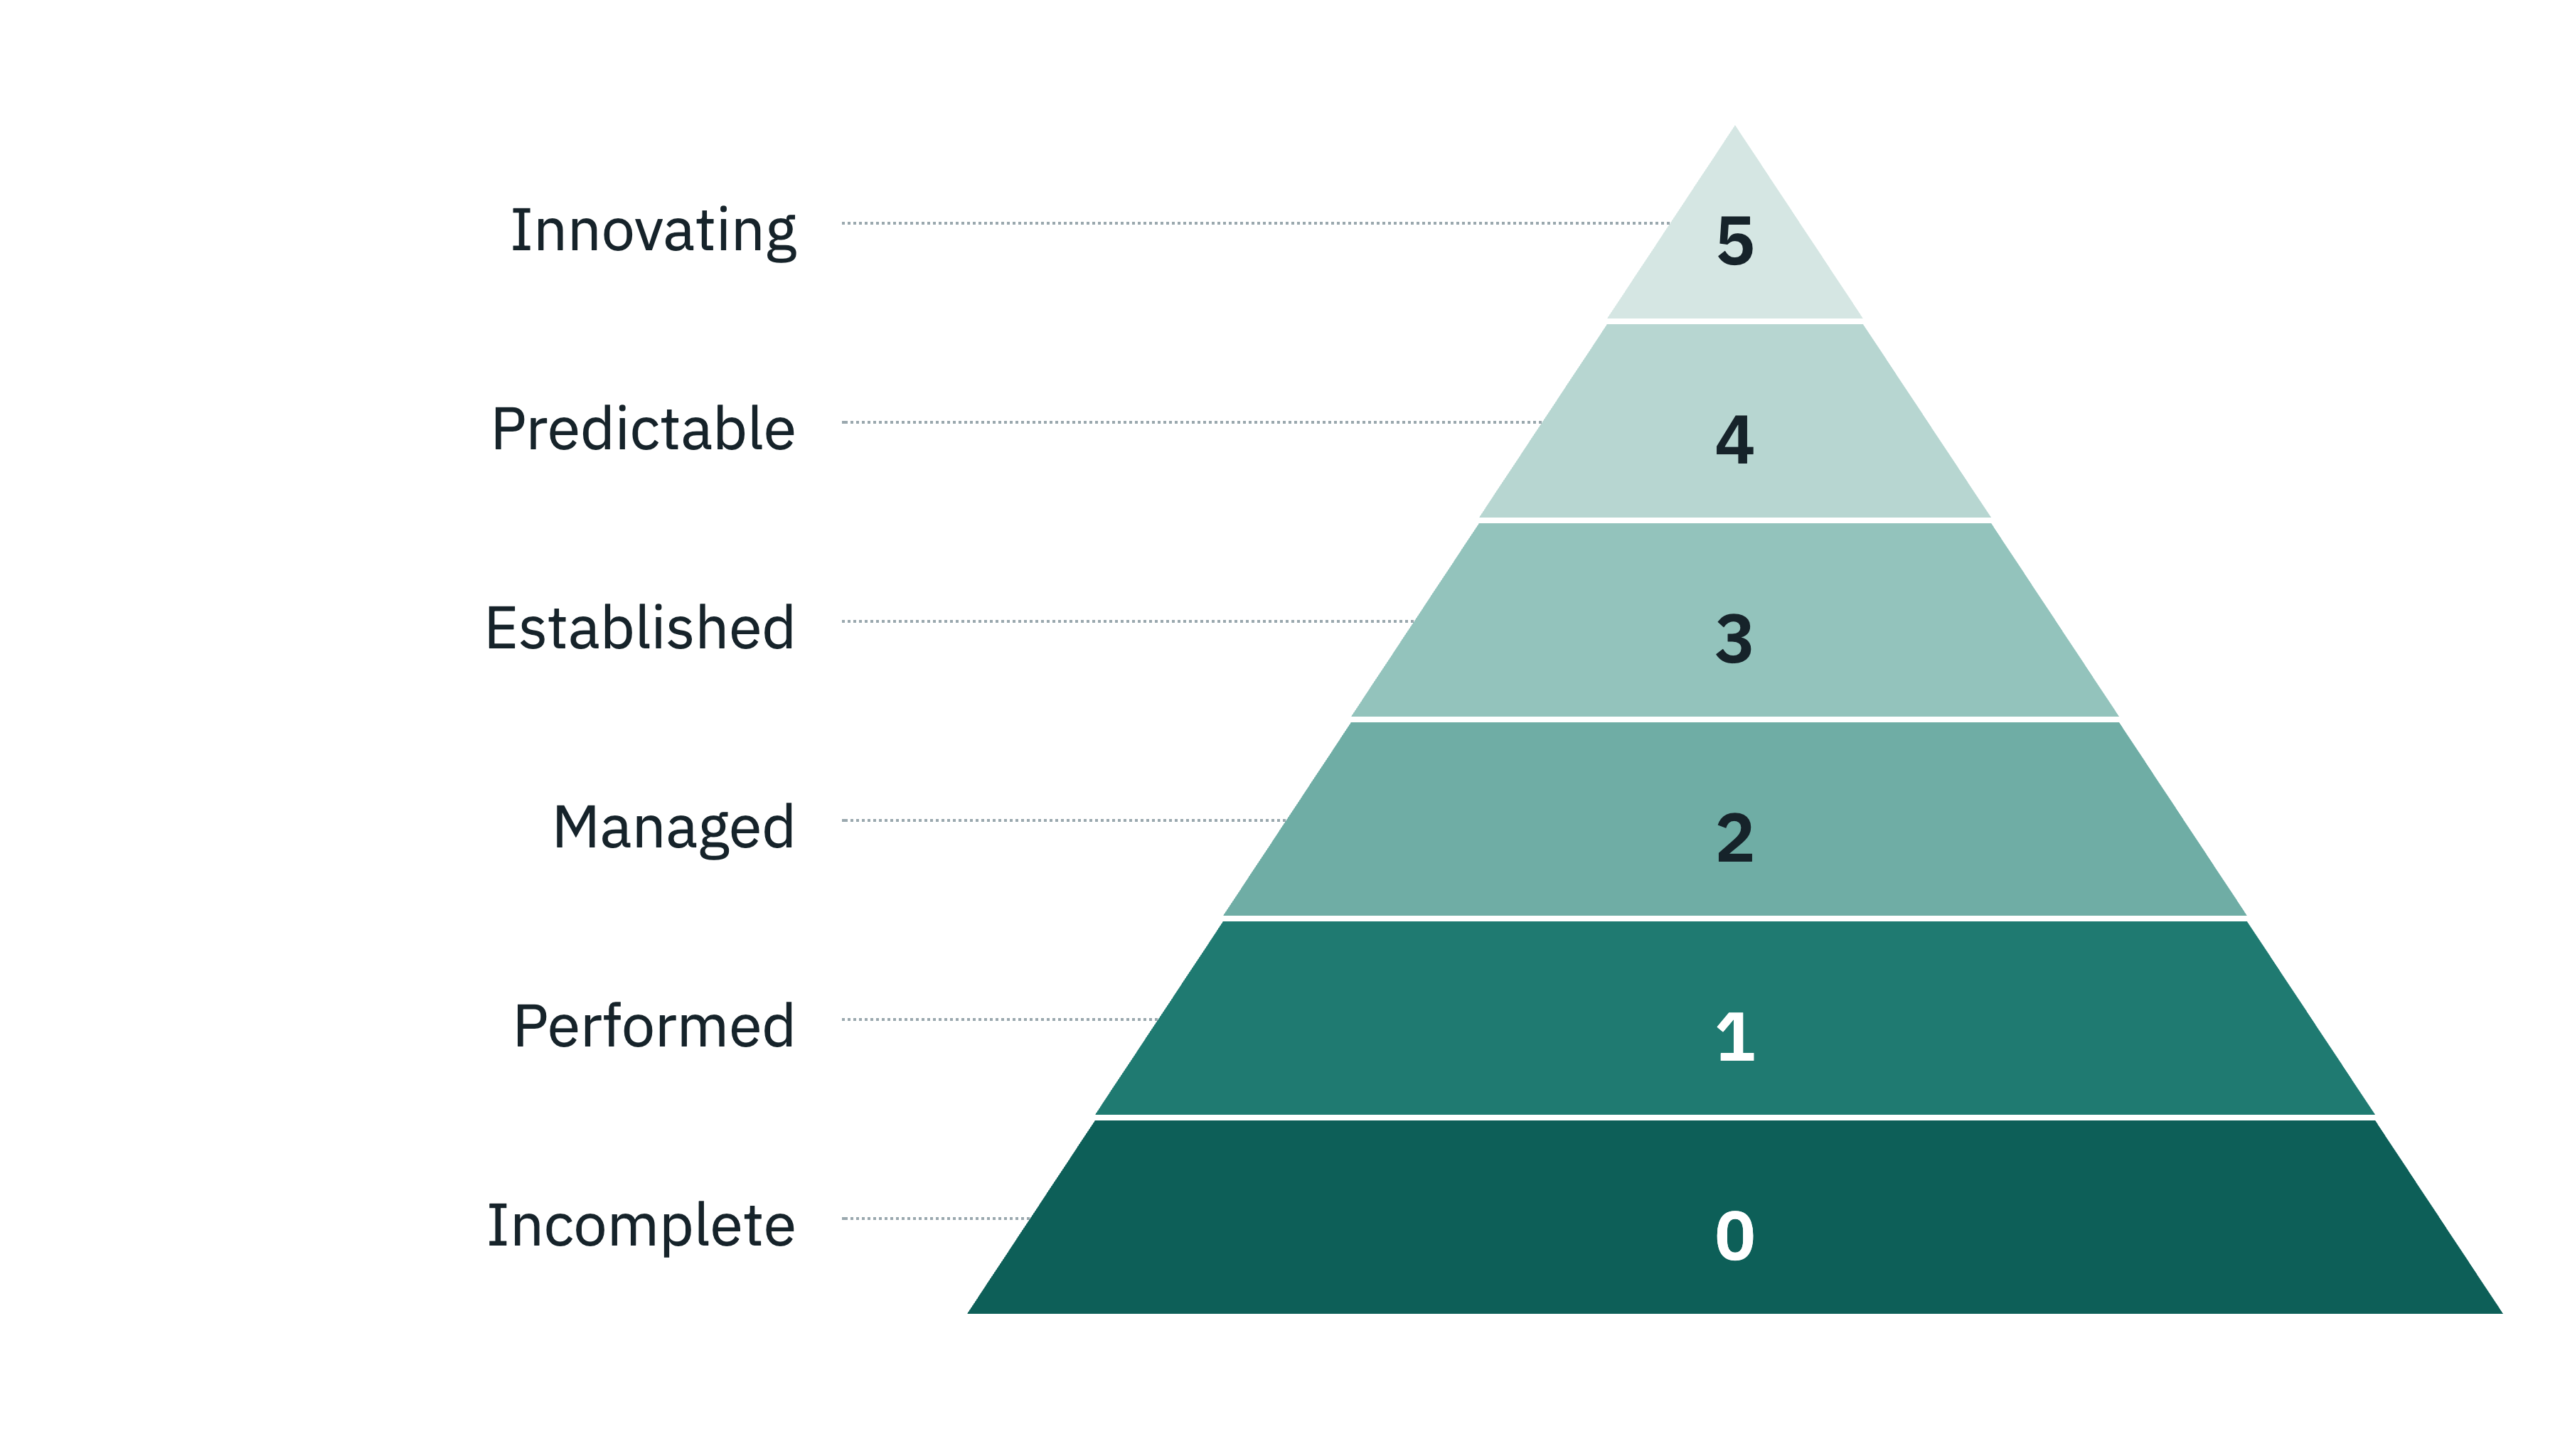
\includegraphics[width=0.6\textwidth]{src/levels.png}
  \caption{The six ASPICE capability levels, from Level~0 (Incomplete) to Level~5 (Innovating).
  Adapted from the official Automotive SPICE process model~\cite{vdaqmc_website}.}
  \label{fig:capability-levels}
\end{figure}

\begin{description}
  \item[L0, Incomplete] The process is not implemented or is not effective.
  \item[L1, Performed] The process is effective in achieving the purpose. Evidence for this level
  is found in the base practices which outline, for each of the SWE.1--SWE.6 processes, the
  activities that are required for the process.
  \item[L2, Managed] The process is not only carried out, but planned and monitored, and the work
  products are appropriately controlled.
  \item[L3, Established] The process is documented and is customised and applied throughout the
  organisation.
  \item[L4, Predictable] The process will function within certain quantitative limits, and the
  operation of the process will be predictable.
  \item[L5, Innovating] The process is continually improved throughout the organisation through
  quantitative feedback.
\end{description}

This thesis includes the first three levels (L1--L3). The levels L4 and L5 are not included: They
would need evidence gathered over multiple projects over time, which a single stakeholder is
unlikely to be able to provide in a single session~\cite{vdaqmc2023pam}.

\subsection{The Traditional (Manual) Assessment Procedure}

An ASPICE assessment is conducted by an assessment team, led by a certified assessor, that
evaluates work products (documents, models, test records, etc.) and interviews project staff to identify if each base
practice and generic practice has been met. The percentage of evidence found is then used to
assign scores to each of the process attributes on an ordinal scale from Not achieved to Fully
achieved~\cite{vdaqmc2023pam}. The outcome is a capability profile which gives a rating for each
process and level that has been measured in the assessment.

This procedure is performed once or twice in a project, at a specific time and results in a
judgment~\cite{vdaqmc2023pam,murphy_aspice_0to60}. There is, however, no inbuilt process to
ensure that the processes that have been assessed continue to be followed between assessments.

\subsection{Pain Points of Manual Assessment (Time, Consistency, Continuity)}

This is a procedure that has three main consequences. First, feedback is only given when an
assessment occurs -- feedback on a process weakness that occurred the following week from an
assessment may not be known until the next assessment. Second, fixing a problem at the end of the
development cycle is much more costly than fixing the same problem at the start of the
development cycle, since other work may be dependent on the incorrect requirement or design at
the time the problem is discovered. Third, an assessor's depth of a manual assessment is limited
by the amount of time that he or she has. An assessor does not have a lot of time to spend onsite
so a sample of evidence must be examined instead of all evidence; thus, the extent of the sample
of evidence examined during a particular audit is dependent on the questions the assessor decides
to ask.

Datsogiannis~\cite{datsogiannis2024early} recognizes the same gap first, which is that once a
supplier is certified, there is no way to directly monitor the supplier's process to ensure that
it continues to meet the requirements, and therefore organizations often use generic project
management or defect-tracking systems, which were not designed to perform process assessment.
This is the particular issue that will be tackled in the rest of this thesis.

\section{Recommender Systems}

A recommender system is used to filter out a small, relevant subset of items from a large pool of
items and for a specific user and context~\cite{lu2012recommendersystems}. The same fundamental
principle is used in this thesis to determine which next question to ask out of the ASPICE
questions.

\subsection{Content-Based and Collaborative Filtering Approaches}

There are two classical approaches for content-based filtering and collaborative filtering but
none is directly applicable to this thesis~\cite{lu2012recommendersystems}. Both require a
consistent past preference -- either of the stakeholder or other users. The next time this system
is deployed, however, there is no history with regard to the questions and the stakeholders that
answer them, the same cold-start problem that affects any freshly deployed recommender
system~\cite{rama2019coldstart}. The analysis of this comparison is described in
Chapter~\ref{chap:sota}.

\subsection{Sequential and Adaptive Recommendation}

Sequential, Adaptive recommendation is better fit. In this case, one item is selected, the
outcome is observed, and the outcome is then used to determine the next item to select during the
session and so on. This is the approach that was taken in this thesis, and is what is being used
in the approach described in the next section~\cite{datsogiannis2024early};
Chapter~\ref{chap:sota} will discuss the previous work which led to this in more detail.

\section{Multi-Armed Bandits}

Multi-armed bandit is a repeated decision problem where an agent has to select one of several
options on each round which gives him a reward, and maximizes his cumulative reward over the
rounds~\cite{naeem2020gentleintro,sutton2018reinforcement}. Each of these selectable options is
called an arm. The name is based on a string of slot machines, that are sometimes referred to as
``one-armed bandits'', and have an unknown and possibly different payout rate: pulling one of
these machines' single arms is one round, and choosing which machine to pull is choosing an arm.

\subsection{The Exploration--Exploitation Trade-off}

The main difficulty in a bandit problem is that the agent has no information about in advance
which arm will yield the highest reward. It thus needs to invest some rounds in trying out arms
over which it has limited knowledge (exploring) and other rounds in choosing the arm that has
performed best so far (exploiting). Importantly, it is only able to observe the reward for the
arm it selected, the partial-feedback setting common to online decision
problems~\cite{datsogiannis2024early,naeem2020gentleintro,bechavod2019partialfeedback}. It can be expensive if this
balance is not achieved. If one pursues an arm too early, he may end up with a random looking
arm, and if he waits too long to explore, he may miss out on an opportunity to get a good arm.

There are a number of algorithms that try to solve this trade-off in various ways:

\begin{description}
  \item[Epoch-Greedy] Is an algorithm that alternates between regular epochs of exploration and
  exploitation~\cite{langford2007epochgreedy}.
  \item[Softmax / $\epsilon$-greedy] Selects the current best arm with a fixed or decreasing
  probability, but selects a random arm with the rest of the
  time~\cite{tokic2011valuedifference}.
  \item[Thompson Sampling] The Thompson Sampling algorithm keeps an updated probability of the
  effectiveness for each arm, and draws from that probability to decide which arm to
  attempt~\cite{agrawal2013thompson}.
  \item[Upper Confidence Bound (UCB)] Each arm's estimated reward is incremented by a bonus that
  depends on the level of uncertainty associated with that reward; an arm is more likely to be
  chosen if it looks like it's very rewarding, or if it hasn't been played enough to determine
  whether it's~\cite{auer2002confidence}.
\end{description}

\subsection{From Stateless Bandits to Contextual Bandits}

All of the algorithms described above assume that each iteration of the problem is identical,
meaning that the same set of arms is used, and the same reward is given for each arm. This is
not the case here. The question that is most informative depends on who is questioning (which
stakeholder) and what has already been discussed in the session, including which processes and
capability levels have already been discussed~\cite{datsogiannis2024early}. This assumption is
eliminated by a contextual multi-armed bandit (CMAB). Before each round, the agent sees a
context, a set of features that represent the current situation, and estimates the reward of
each arm as a function of that context~\cite{li2010contextual}. The context vector is a vector
that represents a stakeholder's role and the status of the current assessment session (see
Chapter~\ref{chap:architecture} for the full definition). This approach to framing questions in
this way allows for the same set of questions to be used for all stakeholder roles, as the
algorithm learns what questions are relevant for what context, and not all
users~\cite{gutowski2018contextenhancement}.


\subsection{LinUCB: Mathematical Foundations}

In this thesis, a contextual bandit algorithm called LinUCB has been assumed in which the
expected reward for each arm can be modeled as a linear function of the context
vector~\cite{li2010contextual,huang2016linucb}, written throughout as $x$: a $d$-dimensional
vector of features describing the current situation (Section~\ref{sec:cmab-engine} defines the
20 features this thesis actually uses). Each arm $a$ has two learned quantities, a $d \times d$
matrix $A_a$ and a $d$-dimensional vector $b_a$, with $d$ the number of context features. These
quantities are used to estimate a weight vector $\theta_a$ (one per arm, describing how much each
context feature drives that arm's reward) from,

\[
\theta_a = A_a^{-1} b_a ,
\]

and scores arm $a$ for the current context as

\[
\mathrm{UCB}_a(x) = \theta_a^\top x \; + \; \alpha \sqrt{x^\top A_a^{-1} x} .
\]

Here, the superscript $\top$ denotes the transpose, so $\theta_a^\top x$ is an ordinary dot
product between the weight vector and the context vector, reducing them to a single number. This
first term is the best guess the algorithm has for the reward that it
would receive if it pulled arm $a$ in this context. The second term is larger if $A_a$ has little
information about contexts like $x$, thus adding value to arms in which the algorithm is not
sure. This uncertainty bonus is given a greater or lesser degree of influence through the
exploration coefficient $\alpha$, which is compared to the direct reward
estimate~\cite{li2010contextual}. At each round, LinUCB picks the arm with the largest
$\mathrm{UCB}_a(x)$.

Once the chosen arm has returned a reward $r$, the parameter of the arm is changed:

\[
A_a \leftarrow A_a + x x^\top , \qquad b_a \leftarrow b_a + r\, x .
\]

Every new question is started with the same, maximally uncertain estimate, $A_a = I$ (the
identity matrix) and $b_a = \mathbf{0}$.

The uncertainty bonus in $\mathrm{UCB}_a(x)$ provides a level playing field for the new question
to be chosen in the first couple of times it can be played~\cite{li2010contextual}. The update
rule is only dependent on matrix and vector arithmetic and the arm selection is a deterministic
function of the variables $A_a$, $b_a$, and $x$, so that the same context and the same history
will always yield the same arm choice. One of the reasons why LinUCB is a suitable choice for a
thesis with the requirement of repeatability and reproducibility is this property.

\section{Chapter Summary}

This thesis addresses six software engineering processes and base practices at three capability
levels, typically assessed by a person in a scheduled assessment, in the context of ASPICE. The
general outline of the proposed solution is suggested by recommender systems, especially the
sequential and adaptive ones: rather than asking all the questions, the recommender system asks
a few questions that are informative. The mechanism used in this thesis is a contextual bandit,
and in particular LinUCB: a way to choose the next question based on the answers it has
received, what has been answered already in the session, and how this can be improved over the
course of more sessions. In Chapter~\ref{chap:sota}, this thesis is placed in the context of the
most similar previous research, and Chapter~\ref{chap:architecture} details how these three
ideas are integrated into the real system.

\chapter{State of the Art}
\label{chap:sota}
% \input{src/state_of_the_art}

In this chapter, this research is placed in its relation to the most similar work already been
done. It starts with a short introduction to ASPICE and the assessment in practice. It then
explains the two papers by Datsogiannis~\cite{datsogiannis2024early,datsogiannis2025recommender}
which this thesis relies on most directly, along with the
diagrams which explain their approach. Lastly, it connects the various approaches in a comparison
table and describes the research gap that this thesis will fill.

\section{ASPICE and Current Assessment Practice}

The typical ASPICE assessment process was described in Chapter~\ref{chap:background}. In
practice, the process is conducted as a periodic audit where an assessment team, led by a
certified assessor, visits a project at specific intervals, collects evidence of base practices in accordance with the
SWE.1--SWE.6 and rates the capability of the project until the next
audit~\cite{vdaqmc2023pam,murphy_aspice_0to60}. This is the standard to which the rest of this
chapter is contrasted. Datsogiannis~\cite{datsogiannis2024early} points out that the biggest
drawback is that the certification under ASPICE does not offer an inbuilt mechanism to track the
compliance of the process once it has been certified. Consequently, organisations tend to rely on
project management tools or defect tracking systems which were not intended to be used to
identify if a particular base practice is being observed or not. The following section thus
examines the way in which Datsogiannis suggests to fill this gap.

The structure of the indicators that underlie that rating are shown in
Figure~\ref{fig:soa-aspice-indicators}. The purpose and outcomes of a process are derived from
the PRM and the evidence used by an assessor to rate the process is added to the PAM. This
evidence for Capability Level~1 contains process performance indicators, base practices, and
work products that are specific to each process. At above level~1 the assessment is based on
process capability indicators, generic practices and generic resources which are applicable
across processes~\cite{vectorconsulting_aspice}.

\begin{figure}[h]
  \centering
  
\includegraphics[width=0.8\textwidth]{src/Soa_Aspice_1.png}
  \caption{How PRM and PAM indicators relate to capability levels: base practices and work
  products evidence Capability Level~1, while generic practices and generic resources evidence
  every level above it. Adapted from Vector Consulting~\cite{vectorconsulting_aspice}.}
  \label{fig:soa-aspice-indicators}
\end{figure}

\section{Prior Work: CMAB-Based Recommendation for Automotive Process Assessment}

Two papers from TU Chemnitz suggest to use a contextual multi-armed bandit to choose assessment
questions for automotive software processes. The first paper presents the idea and its
architecture~\cite{datsogiannis2024early} and the second paper extends the idea with a real
example of comparing bandit algorithms with simulated data~\cite{datsogiannis2025recommender}.
The two papers are the closest prior art to this thesis and the design described in
Chapter~\ref{chap:architecture} is a development of those two papers.

\subsection{2024: A Dynamic Survey Model for Automotive Process Evaluation}

Datsogiannis~\cite{datsogiannis2024early} recommends a system that handles a dynamic
questionnaire, instead of a fixed one. The questions are based on the literature search on automotive
software development metrics, automotive specific studies, ASPICE (SYS.1--SYS.5, SWE.1--SWE.6,
VAL.1, PIM.3), ISTQB~\cite{istqb_website} and documented OEM electrical/electronic processes.
Answers are given a value and each question has a weight representing its importance. The higher
the score, the worse the answer; the most revealing answer will have the highest score. At this
stage, the question is packaged as shown in Figure~\ref{fig:soa-evaluation-packet}: It includes
an identifier, roles who can ask it, roles who'll be affected by a failed answer, its weight,
question and answer payloads, and the actual answer provided.

\begin{figure}[h]
  \centering
  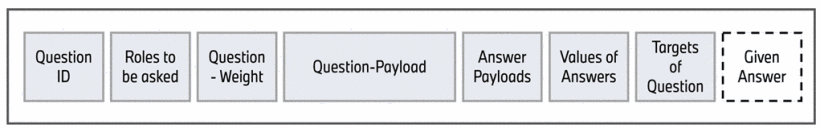
\includegraphics[width=\textwidth]{src/Soa_2.png}
  \caption{Structure of an evaluation packet, from question identifier to given answer.
  Reproduced from~\cite{datsogiannis2024early}.}
  \label{fig:soa-evaluation-packet}
\end{figure}

In each development cycle, a CMAB agent chooses which questions to ask, and which of the seven
roles of the stakeholders will respond to those questions. This is shown in
Figure~\ref{fig:soa-cmab-workflow} as a continuous serving loop instead of a single computation:
The agent explores the current context, and the resulting context, action, reward is logged and
added to the training data. A new model is then learned online from the data and the new model is
deployed back to the agent before the next round.

\begin{figure}[h]
  \centering
  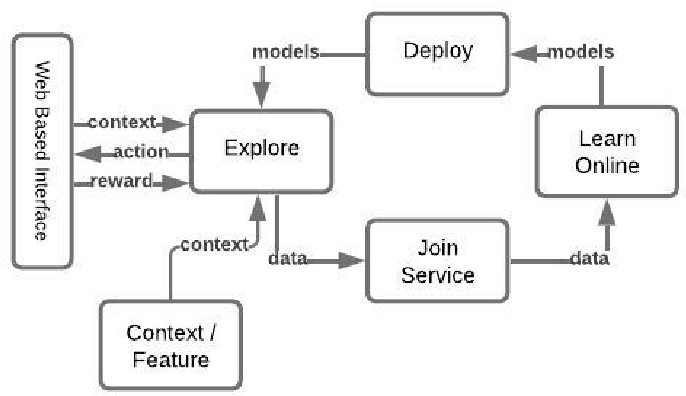
\includegraphics[width=0.65\textwidth]{src/Soa_3.png}
  \caption{The CMAB serving loop: explore, log context/action/reward, learn a new model online,
  deploy it, and explore again. Reproduced from~\cite{datsogiannis2024early}.}
  \label{fig:soa-cmab-workflow}
\end{figure}

The paper also suggests a three banded (red, yellow, green) traffic-light categorization of the
results to enable the use of two thresholds on a calculated score. But it doesn't go so far as a
complete implementation. The conclusion of its own paper confirms that the concept was still
under development at the time of writing and training and evaluation outcomes would be published
later~\cite{datsogiannis2024early}.

Relevance to this thesis: there are two design aspects from this paper that are carried
over directly. First, each question carries a weight and each answer a value, so that the answers
obtained in a session can be translated into a number without further interpretation. Second, the
reward payoff for the CMAB agent is such that the worst response to the most important question
would receive the maximum reward. This way, the agent is led to questions that are more likely to
reveal a genuine weakness and not just a question that is easy to answer. Unlike this paper, the
three-band classifier is extended to a four-band classifier
(Chapter~\ref{chap:architecture}), and the resulting system is implemented and tested.

\subsection{2025: Algorithm Benchmarking on Simulated Data}

In a similar fashion, Datsogiannis~\cite{datsogiannis2025recommender} extends the concept with a
pool of 137 questions and compares three bandit algorithms directly: $\epsilon$-greedy, LinUCB
and Thompson Sampling. As there was no real deployment at that point, the
comparison is based on a simulated environment that mimics the behavior of real software
releases. There are four different scenarios that alter the degree of variation in the underlying
set of process deficiencies between rounds: 0\%, 10\%, 30\%, and 50\% of the process deficiencies
change between rounds. All algorithms were separately tuned for each scenario (as summarized in
Figure~\ref{fig:soa-tuning-tree}) and then compared over 1{,}000 simulated rounds, using the
following measures: cumulative reward, average reward per round, and percentage of rewards in
four score bands (shown for one scenario in Figure~\ref{fig:soa-reward-distribution}).
Table~\ref{tab:recommender-results} shows the results for the least volatile and most volatile
cases with the best tuning for each algorithm.

\begin{figure}[h]
  \centering
  
\includegraphics[width=0.9\textwidth]{src/Soa_4.png}
  \caption{Best tuning parameter found for each of the three algorithms, in each of the four
  deficiency-change scenarios. Reproduced from~\cite{datsogiannis2025recommender}.}
  \label{fig:soa-tuning-tree}
\end{figure}

\begin{figure}[h]
  \centering
  
\includegraphics[width=0.7\textwidth]{src/Soa_5.png}
  \caption{Distribution of $\epsilon$-greedy's rewards at 0\% deficiency change, across four
  score bands. Reproduced from~\cite{datsogiannis2025recommender}.}
  \label{fig:soa-reward-distribution}
\end{figure}

\begin{table}[h]
\centering
\rowcolors{2}{green!5}{white}
\begin{tabular}{l l c c}
\toprule
\rowcolor{green!55!black}
\thw{Scenario} & \thw{Algorithm} & \thw{Tuning} & \thw{Rewards $>$ 0.75} \\
\midrule
0\% change  & $\epsilon$-greedy & $\epsilon=0.5$ & 47.2\% \\
            & LinUCB            & $\alpha=0.1$   & 34.4\% \\
            & Thompson Sampling & $\alpha=0.5$   & 36.7\% \\
\midrule
50\% change & $\epsilon$-greedy & $\epsilon=0.5$ & 25.3\% \\
            & LinUCB            & $\alpha=0.1$   & 24.3\% \\
            & Thompson Sampling & $\alpha=5.0$   & 23.9\% \\
\bottomrule
\end{tabular}
\caption{Simulated algorithm comparison at 0\% and 50\% deficiency-change rate, reproduced
from~\cite{datsogiannis2025recommender}. The right-hand column is the share of rewards that fell
above 0.75, the band representing the most important questions paired with the worst answers.}
\label{tab:recommender-results}
\end{table}

The share of high-reward outcomes is the same across all four scenarios with $\epsilon$-greedy:
$\epsilon$-greedy consistently has the largest share of high-reward outcomes. However, the
benefit it has over LinUCB decreases as the deficiency-change rate rises, from approximately 13
percentage points at 0\% change to approximately 1 percentage point at 50\%
change~\cite{datsogiannis2025recommender}. The tuning parameter, $\alpha$, is also different for
different scenarios, with the value of $0.1$ in most of the scenarios and $\alpha = 2.0$ in the
30\%-change scenario. The two results are not actual deployment results. But the results of a
real automotive development environment would be reported in another paper, according to the
paper itself.

Relevance to this thesis: this is the most similar available comparison of the
performance of LinUCB (the algorithm used in this thesis) compared to other methods. It is thus
not a standard that can be disregarded just because LinUCB did not perform the best in the
simulation. In Section~\ref{sec:cross-comparison}, that result is taken into account, but the
reasons for this choice of thesis are also considered.

\section{Cross-Comparison and the Recommended Method for This Thesis}
\label{sec:cross-comparison}

Table~\ref{tab:cross-comparison} shows a comparison between manual ASPICE practice, the previous
work described above, and this thesis, for the properties that are important for continuous and
automatic process assessment. The \cmark\ means that a property is met and the \xmark\ means
that a property is not met; the other rows are properties that are not binary. Both manual
practice and the previous work meet some of these requirements, but not all. This thesis is the
only one of the three that meets all the criteria that can be checked, as it focuses its scope
while still being implemented and evaluated.

\begin{table}[h]
\centering
\rowcolors{2}{green!5}{white}
\begin{tabular}{p{2.7cm} p{3.0cm} p{3.6cm} p{3.6cm}}
\toprule
\rowcolor{green!55!black}
\thw{Aspect} & \thw{ASPICE (current practice)} &
\thw{Prior work~\cite{datsogiannis2024early,datsogiannis2025recommender}} &
\thw{This thesis} \\
\midrule
Assessment style & Manual, audit-driven & Continuous, question-driven & Continuous,
ASPICE-aligned, web-based \\
Question-based evaluation & \cmark\ Yes, by auditors & \cmark\ Yes, derived from metrics &
\cmark\ Yes, ASPICE base practices turned into questions \\
Structured question database & \xmark\ Not a standardized dataset & \cmark\ Generic questions for
general software & \cmark\ New structured SWE.1--SWE.6 question bank \\
ASPICE scope / focus & \cmark\ Full standard, as needed & \xmark\ SYS.1--SYS.5, SWE.1--SWE.6,
VAL.1, PIM.3 (not SWE-specific) & \cmark\ Explicit SWE.1--SWE.6 mapping only \\
Automated question selection & \xmark\ Human assessor selects & \cmark\ CMAB agent (three
algorithms compared) & \cmark\ CMAB agent (LinUCB) \\
Early feedback & \xmark\ Mostly late, at audit time & \cmark\ Early evaluation, in simulation &
\cmark\ Early SWE weakness visibility \\
Evaluation basis & Not applicable (the standard itself) & \xmark\ Simulated data only & \cmark\
Real pilot audit sessions \\
\bottomrule
\end{tabular}
\caption{Manual ASPICE practice, prior CMAB-based work, and this thesis, compared.}
\label{tab:cross-comparison}
\end{table}

There are three conscious decisions made in regards to the previous work in this thesis. First,
it reduces the scope of ASPICE from four process groups to just one, SWE.1--SWE.6, thereby
allowing the question bank in Chapter~\ref{chap:implementation} to be constructed directly from
the base practices of this group, instead of a more general literature review. Second, it uses
LinUCB in particular, instead of comparing several algorithms: LinUCB's score is a deterministic
function of the session context, so a given session's question choices can always be recomputed
and explained after the fact, and it is natively context-aware, scoring each question directly
from the session-state vector rather than bolting context on separately, unlike $\epsilon$-greedy
or Thompson Sampling. This is a deliberate trade-off, not an oversight:
Table~\ref{tab:recommender-results} shows $\epsilon$-greedy scoring higher on raw reward in
simulation, and the full reasoning behind choosing LinUCB regardless, together with how that gap
holds up on real pilot data, is given in Chapter~\ref{chap:architecture} and revisited
empirically in Chapter~\ref{chap:results}. Thirdly, it tests the system with actual
(non-simulated) pilot sessions, while neither of the previous papers does.

The literature is otherwise sparse on the use of recommender systems in the automotive
processes. The nearest non-supervisor prior work is Bader's dissertation on proactive
recommender systems in automotive scenarios~\cite{bader2013proactive} where the recommendations
are made to the driver instead of assessing the process as done by the development team and is
not based on ASPICE.

\section{Research Gap}

The previous sections demonstrate there is clearly a gap. Manual ASPICE assessment does not
offer a way to monitor continuously~\cite{datsogiannis2024early}. As far as we know, the closest
previous work is an ongoing, CMAB-based approach, which has not yet been used as a working
system, but only tested by
simulation~\cite{datsogiannis2024early,datsogiannis2025recommender}. The integration of a
continuous, automated and stakeholder-driven recommendation system and the explicit
implementation of ASPICE SWE.1--SWE.6 has not been published together with an evaluation based
on real assessment sessions. This is the space this thesis aims to fill.

\section{Chapter Summary}

Manual ASPICE assessment gives clear ratings, they are awarded at audit time only. The previous
studies that were reviewed in this chapter have demonstrated the feasibility of a questionnaire
driven by the CMAB concept, both conceptually and in a synthetic simulation that mimics software
releases, but have not yet been implemented in a working deployment. This thesis focuses on this
space in particular for SWE.1--SWE.6: it takes the same concept, restricts the scope of the
ASPICE, makes a single choice of algorithm, and tests the system itself end to end, on sessions
actually run through the live application, rather than on a simulated environment. ``Real'' here
means exactly that: an actual working system exercised by actual sessions, not an independent
field deployment -- the pilot was self-administered by the author across all seven stakeholder
roles, and Chapter~\ref{chap:results}'s Threats to Validity section examines what that does and
does not prove. The way that that system is constructed is explained in
Chapter~\ref{chap:architecture}.

\chapter{System Architecture and Design}
\label{chap:architecture}
% \input{src/architecture}

This chapter deals with the system design and starts with the requirements that the system must
meet, then works its way through the overall architecture, the question bank and assessment
model, the design of the database, the CMAB recommendation engine, and the weakness classifier
that transforms stakeholder answers into a result. It also addresses the API design and user
interface design, and concludes with the key design decisions and trade-offs.

\section{Requirements Analysis}
\label{sec:requirements-analysis}

\subsection{Functional Requirements}

\begin{itemize}
  \item \textbf{FR1.} The system shall replace the manual, periodic ASPICE assessment procedure
  with a continuous and automated assessment procedure that is aligned with the ASPICE
  SWE.1--SWE.6 standard.
  \item \textbf{FR2.} Stakeholders shall be able to register, log-in, and participate in an
  evaluation session.
  \item \textbf{FR3.} The system shall have a structured question bank on ASPICE SWE.1--SWE.6.
  \item \textbf{FR4.} Stakeholders shall only be asked questions that are relevant to their role
  in the system.
  \item \textbf{FR5.} The system shall automatically identify the gaps in the processes.
  \item \textbf{FR6.} The system shall present the assessment results to the stakeholder in a
  clear way.
\end{itemize}

\subsection{Non-Functional Requirements}

\begin{itemize}
  \item \textbf{NFR1 (Determinism).} Question selection shall be deterministic -- for the same
  input (context, model state), the system shall always return the same result, so it can be
  reproduced.
  \item \textbf{NFR2 (Traceability).} Each question shall be related to one of the ASPICE
  SWE.1--SWE.6 base practices.
  \item \textbf{NFR3 (Security).} No one shall be able to access the system without
  authentication.
  \item \textbf{NFR4 (Bounded session length).} An assessment session shall have a set number of
  questions, and shall not require a stakeholder to spend more than a reasonable and predictable
  amount of time on it.
\end{itemize}

Table~\ref{tab:fr-traceability} maps each functional requirement back to the research question
it serves, so that the design decisions in the rest of this chapter can be read as direct answers
to Chapter~\ref{chap:introduction}'s research questions rather than as free-standing choices.

\begin{table}[h]
\centering
\rowcolors{2}{green!5}{white}
\begin{tabular}{c p{9.5cm} c}
\toprule
\rowcolor{green!55!black}
\thw{Req.} & \thw{Requirement} & \thw{RQ} \\
\midrule
FR1 & Continuous, automated, ASPICE-aligned assessment (core objective) & RQ1--RQ4 \\
FR2 & Stakeholder signup, login, and session participation (supporting infrastructure) & --- \\
FR3 & Structured SWE.1--SWE.6 question bank & RQ1 \\
FR4 & Role-targeted question selection & RQ2 \\
FR5 & Automatic weakness computation & RQ3 \\
FR6 & Clear presentation of results & RQ4 \\
\bottomrule
\end{tabular}
\caption{Functional requirements mapped to the research questions from
Chapter~\ref{chap:introduction}.}
\label{tab:fr-traceability}
\end{table}

% Optional (not yet added): a UML use-case diagram (actors: Stakeholder, Administrator; use
% cases: Start Session, Answer Question, View Results, View History, Manage Question Bank,
% View Analytics) would visualize this requirements section, but would be a fifth diagram in an
% already diagram-dense, 10--12 page chapter -- add only if there is room after writing the
% rest of the chapter.

\section{System Architecture}

\subsection{Overall Architecture}

Figure~\ref{fig:overall-architecture} shows the system at its highest level. The diagram is
based on the concept architecture originally proposed for this line of
work~\cite{datsogiannis2024early}, and it is still a good fit for the system developed in this
thesis. The system is accessed by the development stakeholders and their manager through a GUI.
Every request goes through a central Model Controller, question selection is delegated to a
Recommendation System, the answers are passed to an Evaluation Model which converts them into a
result, and everything is persistently stored in a Database.

\begin{figure}[h]
  \centering
  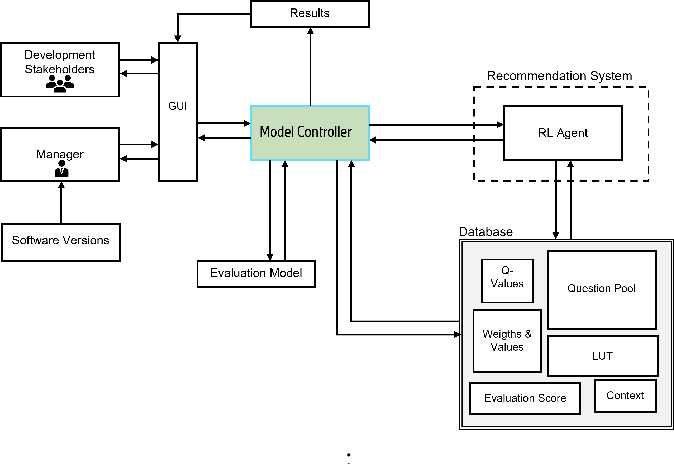
\includegraphics[width=0.85\textwidth]{src/Arch_1.png}
  \caption{Overall system architecture: stakeholders interact through the GUI, the Model
  Controller coordinates the Recommendation System (CMAB agent) and the Evaluation Model, and
  all state is persisted in the Database. Adapted from the concept architecture
  proposed in~\cite{datsogiannis2024early}.}
  \label{fig:overall-architecture}
\end{figure}

The GUI is built with the React frontend. The Model Controller
is the application logic of the FastAPI backend, specifically the audit session service that carries
an audit session from its inception to its completion. The Recommendation System is the CMAB
engine described in Section~\ref{sec:cmab-engine}, using LinUCB to select questions. The
Evaluation Model is the weakness classifier given in Section~\ref{sec:weakness-classification}.
The four labelled sub-parts of the Database correspond directly to the four types of data stored
in this thesis: Question Pool and Weights \& Values are the \texttt{AuditQuestion} and
\texttt{AuditOption} tables, Context and Q-Values are the CMAB context vector and the learned
\texttt{BanditArmState} parameters, and Evaluation Score is the computed \texttt{WeaknessResult}.
One thing worth noting here is that this is a simplified version: the original diagram treats
``Development Stakeholders'' and ``Manager'' as two distinct actor types, and ``Software
Versions'' as a separate input, while in this thesis each stakeholder is instead managed through
a single \texttt{stakeholder\_role} field on the user account, and each audit session is treated
as a stand-alone assessment cycle rather than being tied to one specific tracked software
release.

\subsection{System Components and Responsibilities}

Figure~\ref{fig:component-responsibilities} shows the same architecture as
Figure~\ref{fig:overall-architecture}, but relabelled with the concrete implementation names
introduced above and organised by responsibility instead of by request flow: the GUI becomes
Presentation, the Model Controller is split into API and Audit Session Service (routing and
authentication versus orchestrating the session lifecycle), the Recommendation System is the CMAB
Engine, the Evaluation Model is the Weakness Classifier, and the Database becomes the Data Layer.
Rather than showing how a request moves through these components, as
Figure~\ref{fig:overall-architecture} does, this diagram states what each one is responsible for.

\begin{figure}[h]
  \centering
  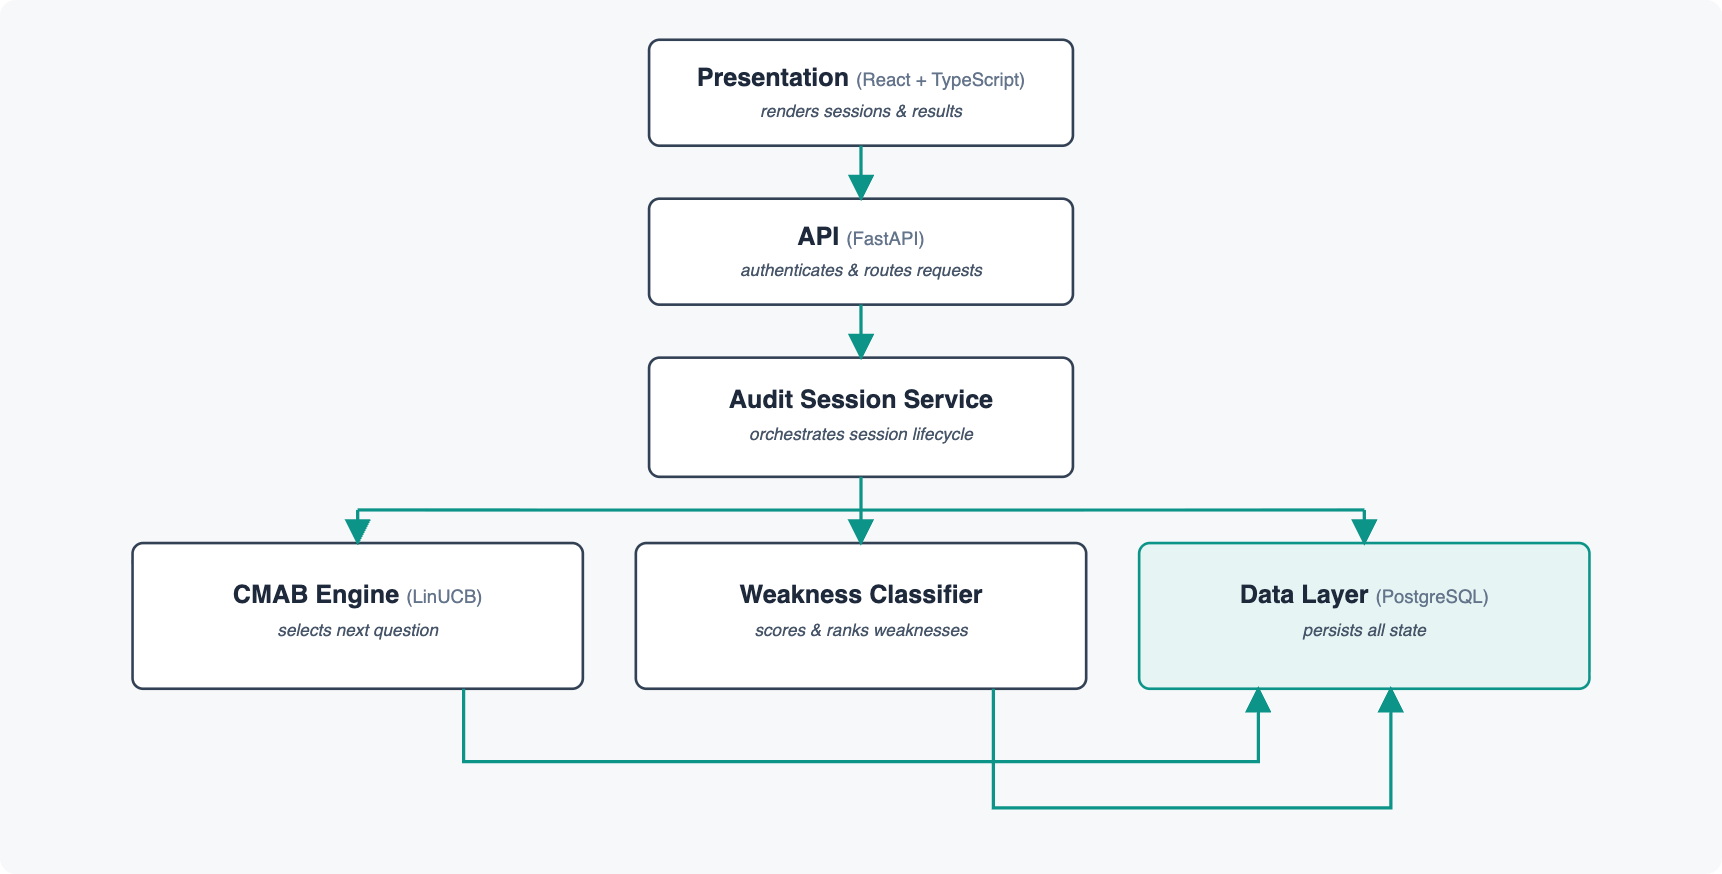
\includegraphics[width=0.90\textwidth]{src/Arch_2.png}
  \caption{System components and their responsibilities. Generated with Claude
  Design~\cite{anthropic_claude_design}.}
  \label{fig:component-responsibilities}
\end{figure}

\subsection{Data and Control Flow}

Figure~\ref{fig:data-control-flow} shows a single example of an answer-submission request as it
passes through the system. Solid arrows are used for control flow and dashed arrows are used for
data reads and writes. The stakeholder's response flows through the API to the audit session
service. The CMAB engine is then updated and, if the session has not reached its question budget,
the system gets the next question from the CMAB engine; otherwise it passes control to the
weakness classifier. Along the way, each component reads from the data layer, and writes to it
when necessary.

\begin{figure}[h]
  \centering
  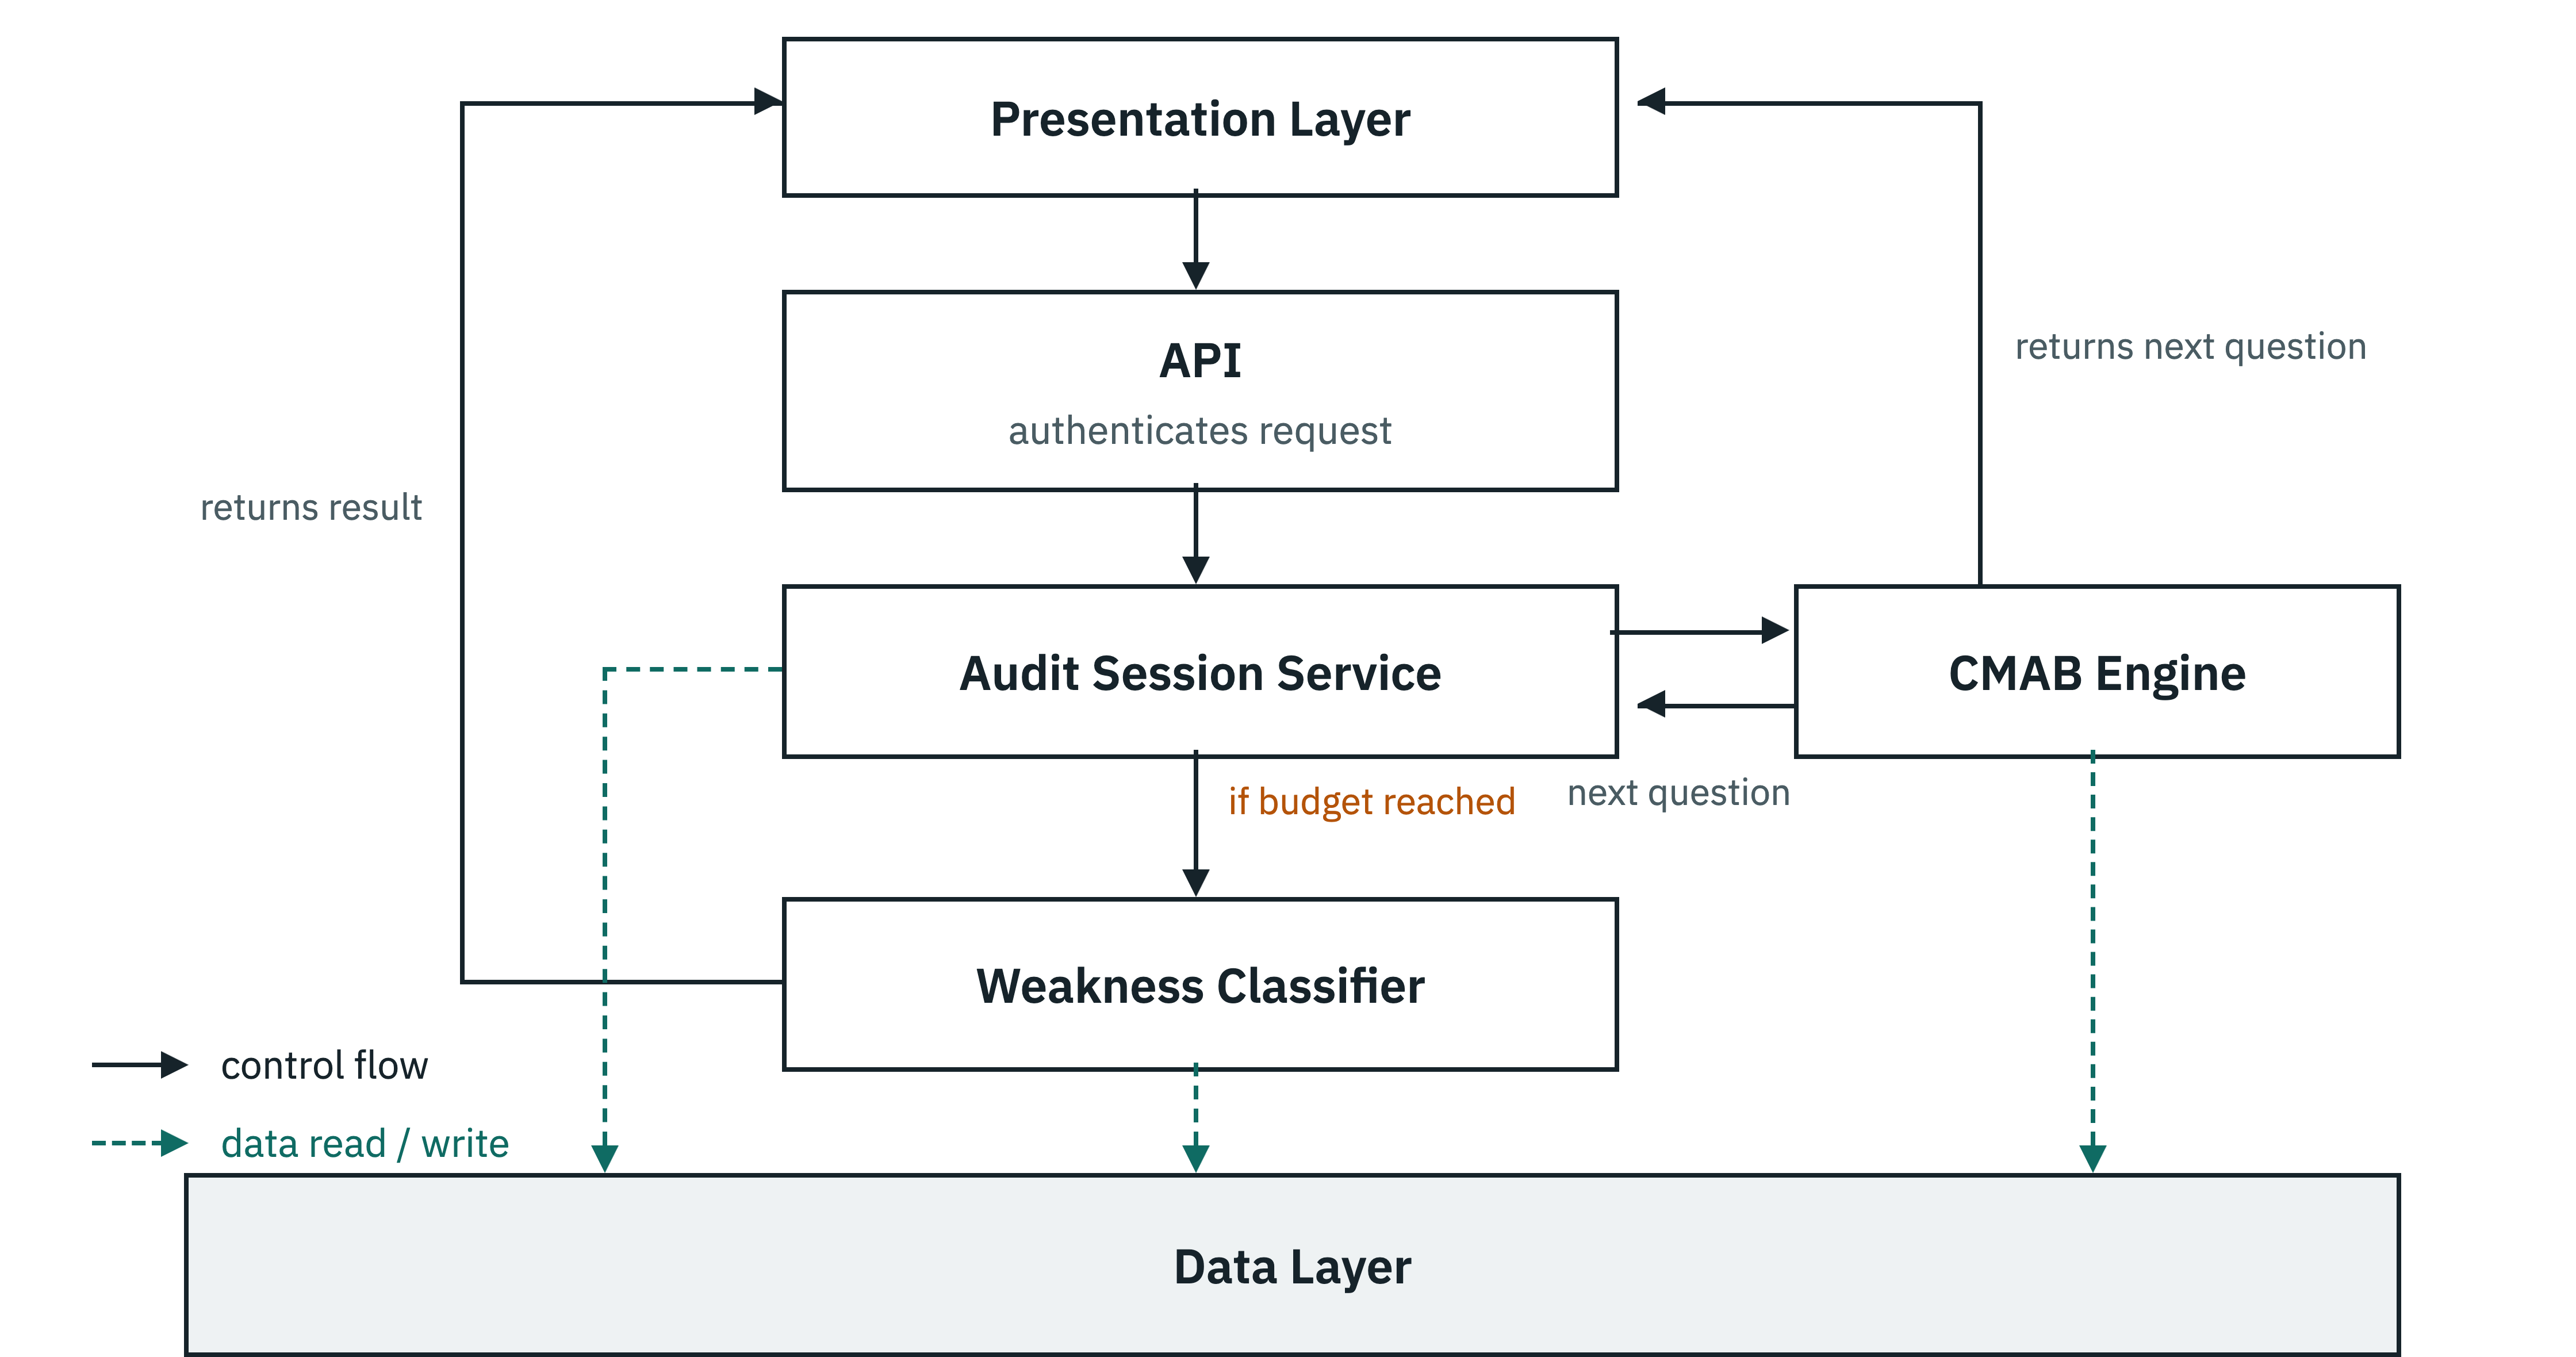
\includegraphics[width=0.90\textwidth]{src/Arch_3.png}
  \caption{Control and data flow for a single answer-submission request. Generated with Claude
  Design~\cite{anthropic_claude_design}.}
  \label{fig:data-control-flow}
\end{figure}

Section~\ref{sec:api-design} and Section~\ref{sec:weakness-classification} come back to this
same flow, once the API contract and the classification logic have been introduced.

\section{Question Bank and Assessment Model}

The question bank is the key to turning the ASPICE standard into something a stakeholder can
answer. This section explains that transformation, using one seeded question,
\texttt{SWE1\_L1\_01}, as an example.

\subsection{ASPICE Base Practice to Question Transformation}

Building the question bank means going through each SWE process's base practices, as defined in
the PAM~\cite{vdaqmc2023pam}, and transforming each one into a question a stakeholder can answer
about their own existing work. SWE.1's first base practice reads: ``Specify software
requirements\ldots\ based on defined characteristics (verifiability, unambiguity, freedom from
design/implementation, no contradictions)''~\cite{vdaqmc2023pam}. In the question bank, this
becomes \texttt{SWE1\_L1\_01}: ``How are software requirements specified for the current
release?'' The question text does not repeat the same characteristics given in the original base
practice; instead, they show up in the variations between the answer options.

\subsection{Question Structure and Traceability}

Each question is stored with a fixed structure: a unique code, its process and capability
level, the base practice ID that links it back to the PAM, the question text, and a
recommendation that is shown when an answer points to a weakness. \texttt{SWE1\_L1\_01}, for
instance, traces to \texttt{SWE.1.BP1}, and its recommendation is to bring in a
requirement-specification template and check the tooling used to manage requirements. This
traceability field is what satisfies NFR2 from Section~\ref{sec:requirements-analysis}, since a
question's justification against the ASPICE standard is one lookup away.

\subsection{Answer Options and Weighting}
\label{sec:answer-weighting}

Each question comes with five predefined answer options, A through E, going from the strongest
practice down to the weakest, each carrying a weight from 0 (practice fully in place) up to 5
(practice effectively absent). One weight is assigned per option so that each of the five
severity levels a stakeholder can pick between has its own distinct value, with 0 corresponding
to the fully-achieved end of the manual ASPICE rating scale (Chapter~\ref{chap:background}) and
higher weights signalling a more serious gap; this higher-is-worse convention is carried over
directly from the prior work this thesis builds on~\cite{datsogiannis2024early}. Table~\ref{tab:example-question}
contains the full set of options for \texttt{SWE1\_L1\_01}. This weight $w$ is what gets
translated into a reward once an option is chosen by the CMAB engine, using $r = w / 4$ capped at
$1.0$, and the same normalized value is later averaged into the process score used by the
weakness classifier (Sections~\ref{sec:cmab-engine} and~\ref{sec:weakness-classification}).

\begin{table}[h]
\centering
\rowcolors{2}{green!5}{white}
\begin{tabular}{c p{8.5cm} c}
\toprule
\rowcolor{green!55!black}
\thw{Option} & \thw{Answer text} & \thw{Weight} \\
\midrule
A & Each requirement is uniquely identified, atomic, verifiable, and references its source & 0 \\
B & Requirements are uniquely identified but verifiability criteria are missing for some & 2 \\
C & Requirements exist as free-text paragraphs without unique IDs & 3 \\
D & Requirements are partially captured in slides or e-mails & 4 \\
E & No formal software requirements set exists & 5 \\
\bottomrule
\end{tabular}
\caption{Answer options and weights for the worked example question \texttt{SWE1\_L1\_01}.}
\label{tab:example-question}
\end{table}

\subsection{Stakeholder Role Assignment}

Each question is also mapped to one or more of seven stakeholder roles: Software Developer,
Software Architect, Project Manager, QA Engineer, Test Engineer, Team Lead, and ASPICE Assessor.
\texttt{SWE1\_L1\_01} is assigned to Software Architect, Software Developer, and QA Engineer, the
roles most likely to be aware of how requirements are actually specified; a Project Manager, on
the other hand, will never be shown this question. This lets the same question bank serve every
stakeholder without asking anyone about work outside their own scope, which satisfies FR4 from
Section~\ref{sec:requirements-analysis}.

\subsection{Question-to-Assessment Flow}

Once a question has been formulated, weighted, and assigned to the appropriate roles, it is
ready for use. At the start of a session, and after every answer, the question bank is reduced
down to those questions still eligible for the stakeholder's role and not yet asked. Each
eligible question is then treated as one arm of the CMAB engine (Section~\ref{sec:cmab-engine}),
which selects among them. These are the same fields defined at question-bank design time, and
they are exactly what the eligibility filter and the weakness classifier read at runtime.

\section{Database Design}

Everything described so far -- the question bank, the roles, the weights -- has to be retained
from one request to the next, and has to be accessible to every stakeholder who starts a session.
This section describes the seven tables that hold that state, and, more importantly, why they
are split up the way they are.

\subsection{Entity-Relationship Model}

Figure~\ref{fig:erd} shows the full database schema. The dashed boundary marks the two tables
that hold learned or derived state, \texttt{WeaknessResult} and \texttt{BanditArmState}, rather
than directly recorded stakeholder input.

\begin{figure}[h]
  \centering
  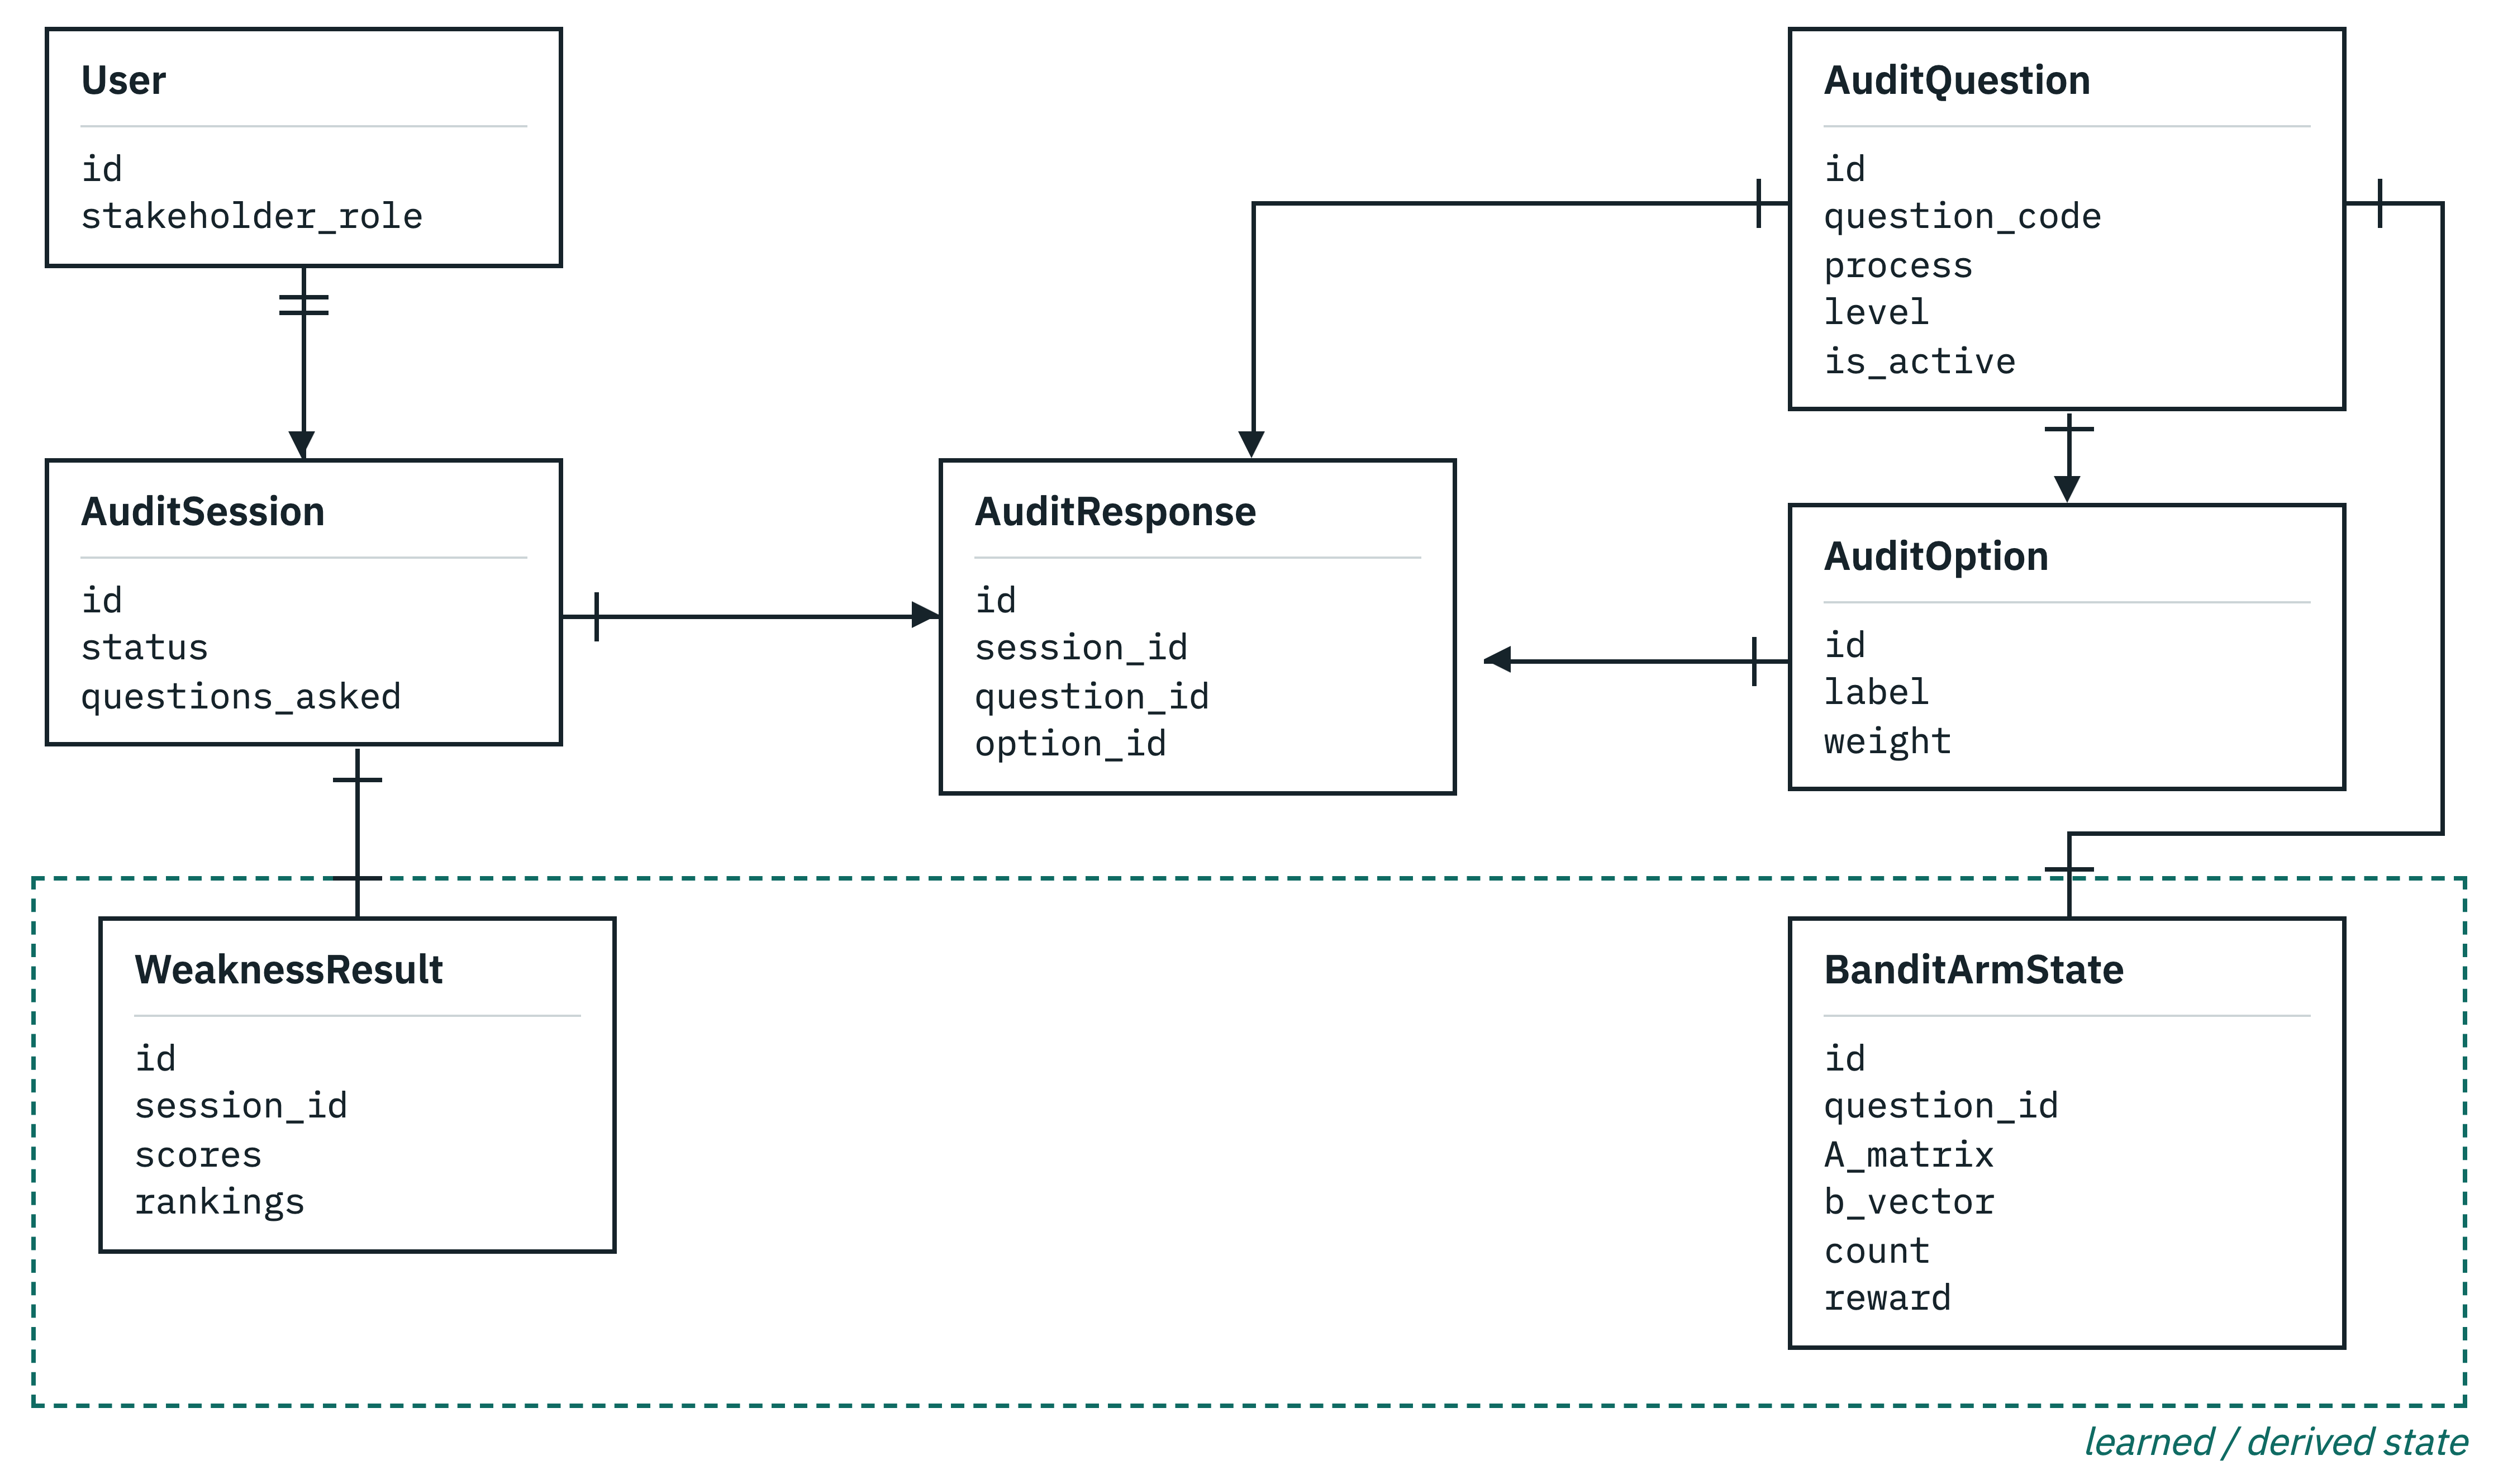
\includegraphics[width=\textwidth]{src/Arch_4.png}
  \caption{Entity-relationship diagram of the database schema. Generated with Claude
  Design~\cite{anthropic_claude_design}.}
  \label{fig:erd}
\end{figure}

At the centre of the schema is a simple chain: a \texttt{User} can start many
\texttt{AuditSession}s over their lifetime, each session stores many \texttt{AuditResponse} rows
as the stakeholder answers questions and selects an \texttt{AuditOption}, and each response
points to the question that was asked and the option that was chosen. Two more tables sit at the
ends of this chain rather than inside it. A \texttt{WeaknessResult} is associated with a single
completed session and is that session's final result. A \texttt{BanditArmState} belongs to a
single question and holds that question's memory of its performance over its lifetime,
independent of any one session or user. In other words: sessions and responses capture what
happened, while results and bandit state capture what was learned from it.

\subsection{User and Question Models}

The \texttt{User} table is the same one the rest of the application already uses for logging in,
except for one extra column: \texttt{stakeholder\_role}. This role is asked for only once, at
signup, and never asked again. Having that single field is what lets every later step --
determining which questions are eligible, and which results a person can see -- happen without
asking the stakeholder to identify their role again.

\texttt{AuditQuestion} is essentially the database representation of the structure described in
Section~\ref{sec:answer-weighting}: the question code, process and capability level, the base
practice ID connecting it to the standard, the question text, the stakeholder roles it applies
to, and the recommendation shown when it is answered poorly. One field is worth calling out
specifically: \texttt{is\_active}. Questions are never permanently deleted -- instead, they are
turned off. This matters because if a question has already been asked and answered by a real
stakeholder, it cannot simply vanish from the database and leave that person's past answer
pointing at nothing. \texttt{AuditOption} sits directly below a question, with one row per answer
choice, each row carrying the label, the option text, and the weight described in
Section~\ref{sec:answer-weighting}.

\subsection{Assessment Session and Response Models}

An \texttt{AuditSession} is kept as simple as possible. It tracks who is taking it, its status
(\texttt{in\_progress}, \texttt{completed}, or \texttt{abandoned}), the maximum number of
questions it can ask before stopping, and the ordered list of questions already served. That last
field is what makes the session self-aware: when it is time to pick the next question, the
system does not have to reconstruct the history from anywhere else, it already knows what has
been asked. Each answer a stakeholder gives becomes its own row in the \texttt{AuditResponse}
table: which session it belongs to, which question was asked, which option was selected, and
when. Keeping one row per answer, rather than folding all answers into the session itself, lets
the weakness classifier later group responses however it needs to -- by process, by level, by
question -- without the session table having to anticipate every possible grouping in advance.

\subsection{Result and CMAB State Models}
\label{sec:result-cmab-models}

The last two tables hold the system's two forms of intelligence, and they are kept deliberately
separate -- from each other and from everything above them.

\texttt{WeaknessResult} is created once per completed session. It keeps the score computed for
every (process, level) pair the session touched, plus a small ranked list of the worst ones. It
is written once, when the session ends, and never changes afterward -- it is a record of a final
judgment, not a value that keeps changing.

\texttt{BanditArmState} works differently. It is not session-specific but question-specific, and
it is updated continually. It keeps the two matrices LinUCB needs for learning, plus a running
count of how often the question has been selected and its cumulative reward. Every stakeholder
who answers that question, in any session, updates the same row.

Keeping \texttt{BanditArmState} separate from \texttt{AuditQuestion} is not just a side effect of
normalization -- it is a deliberate design choice. Question content changes rarely, usually only
when an administrator edits it, while the bandit's learned parameters can change after every
single answer, from every session. Bundling the two into one table would turn editing a
question's wording and updating what the algorithm has learned about it into the same operation,
when they are two distinct things that should stay separate.

\section{CMAB Recommendation Engine}
\label{sec:cmab-engine}

Chapter~\ref{chap:background} introduced the contextual bandit concept in the abstract: arms,
rounds, context, reward. This section relates those concepts to the real objects and decisions
this system actually works with.

\subsection{Mapping Assessment to the CMAB Problem}

Each active \texttt{AuditQuestion} a stakeholder can view is an arm, and each answered question
is a round. The engine is not learning a single ``best question'' -- rather, it learns, per
question, how rewarding that question is for a specific role at a specific point in an assessment
session. This state is kept in the \texttt{BanditArmState} row from
Section~\ref{sec:result-cmab-models}: one row per question, updated after every use of the
question, and never reset.

\subsection{Context Vector}

Before it can score anything, the engine first has to describe the situation it is in: the
20-dimensional context vector $x$ that Chapter~\ref{chap:background} introduced only in the
abstract. The vector is rebuilt fresh every time it is needed, and is never cached: seven
dimensions one-hot encode the stakeholder's role, one dimension measures progress toward the
question budget, six dimensions flag which SWE processes the current session has already
covered, and the last six carry a running weakness score per process based on the answers given
so far. The role dimensions let the same
question be effective for one stakeholder role and irrelevant for another; the coverage flags let
the engine notice, mid-session, that a process has been under-covered, and adjust for it.

\subsection{Arm Eligibility}

Before scoring begins, the engine narrows the active question bank down to admissible arms, recall from earlier in this section that every eligible \texttt{AuditQuestion} is an arm, so this
step decides which questions LinUCB is even allowed to consider next. A question is
admissible only if the question's stakeholder-role list includes the current user's role, and the
question is not already in the list of questions asked during the current session. Both are hard constraints,
enforced directly rather than left for LinUCB to learn to avoid on its own. Filtering first also
means the UCB calculation only has to run over the small number of questions that could
plausibly be asked next.

\subsection{LinUCB Question Selection}

Selection follows the rule introduced in Chapter~\ref{chap:background}: for each eligible arm
$a$, the engine computes its weight vector $\theta_a$ from the two quantities learned for that
arm, a matrix $A_a$ and a vector $b_a$,

\[
\theta_a = A_a^{-1} b_a ,
\]

and scores it as

\[
\mathrm{UCB}_a(x) = \theta_a^\top x + \alpha \sqrt{x^\top A_a^{-1} x}
\]

where $x$ is the 20-feature context vector defined earlier in this section,
$\theta_a^\top x$ is the dot product giving the algorithm's best guess at this arm's reward, and
the square-root term is an uncertainty bonus. The exploration coefficient $\alpha$
starts at $1.0$ -- a single, easy-to-explain hyperparameter that Chapter~\ref{chap:results} comes
back to later. The engine returns the arm with the highest score. Because that score is a
function of $A_a$, $b_a$, and $x$ alone, the same session history always produces the same next
question.

\subsection{Reward Function}

The base reward is the chosen option's weight, from Section~\ref{sec:answer-weighting}, scaled
into the range $0.0$--$1.0$. A coverage bonus of $0.2$ is added on top if the question is the
first this session has asked from its process, and no bonus otherwise. The base reward and the
coverage bonus are combined and then capped at $1.0$. The rationale behind the bonus is simple:
weight alone is not always a safe signal to follow. Without it, an engine chasing high weights
could keep returning to one heavily-weighted process and spend the rest of the session's budget
there, without ever covering the others. The coverage bonus gives the system a direct incentive
to value breadth as well.

\subsection{Online Update and State Persistence}

The reward is applied only to the arm that was selected, following

\[
A_a \leftarrow A_a + x x^\top , \qquad b_a \leftarrow b_a + r\,x .
\]

The updated matrices are written straight back to that question's \texttt{BanditArmState} row, so
the learning produced by the request persists after the request and is never confined to a
single session or user -- every stakeholder who answers that question, in any session, updates
the same row. A question that has never been asked before starts from $A_a = I$ and
$b_a = \mathbf{0}$.

\subsection{Session Budget}

Each \texttt{AuditSession} carries a \texttt{max\_questions} field, twelve by default, but that
number is a ceiling now, not a fixed target. The session does not have to ask the same number of
questions every time: if the system stops finding anything worth flagging in a process, it moves
on instead of asking more questions there, and the session can end well before it reaches that
ceiling. If an answer does point to a weakness, though, the system digs in further -- it keeps
asking related questions in that same process instead of moving straight to the next one.
Control passes to the weakness classifier once the eligible pool runs dry, the system has nothing
left worth asking about, or the ceiling is reached, whichever comes first. This is really the
reason the recommendation engine exists at all: a fixed questionnaire would just ask every
question in the bank regardless of what it finds, but the intent here is different -- to spend a
stakeholder's time only where it's actually needed, digging deeper into the weak spots and
moving past the clean ones.
\section{Weakness Classification and Result Generation}
\label{sec:weakness-classification}

Once a session ends, the CMAB engine has fulfilled its role, and a different, much simpler part
of the system takes over: aggregating the answers into a final result.

\subsection{Response Scoring}

Each answered question contributes one number: the weight of the selected answer, normalized
between $0.0$ and $1.0$ the same way as the reward in Section~\ref{sec:cmab-engine}. The seeded
question bank's weights actually run $0, 2, 3, 4, 5$ rather than $0, 1, 2, 3, 4$: the step from 0
is deliberately larger than the steps afterward, so that the single option representing full
compliance (weight 0) stays clearly separated from every other option, all of which already
represent some degree of weakness, rather than sitting only one point away from the mildest of
them. This is a design choice made when the question bank was authored, not an independently
calibrated scale (Chapter~\ref{chap:conclusion} lists the weights as unvalidated), and one
consequence of it is that a handful of individual answers normalize to just above $1.0$ instead
of stopping exactly at it. This is not a problem downstream, since the classification step in
Section~\ref{sec:classification-thresholds} treats any value past its highest threshold the same
way regardless -- but it is worth stating clearly rather than quietly rounding it away.

\subsection{Process and Capability-Level Scoring}

Each response is associated with exactly one (process, level) pair, taken from the question it
answers. The classifier groups all of a session's responses by that pair and averages the
normalized weights within each group, producing one score for each of the $6 \times 3 = 18$
process-level cells. A pair that the session never covered is not given a score of zero -- it is
left unassessed, since a zero would wrongly suggest the process was checked and found fully
compliant, when it was really just never assessed in this session.

\subsection{Classification and Thresholds}
\label{sec:classification-thresholds}

Each of the 18 scores is assigned to one of four bands, according to the scheme in
Table~\ref{tab:classification-thresholds}. This is the four-band version of the three-band
traffic-light classification introduced earlier in Chapter~\ref{chap:sota}.

\begin{table}[h]
\centering
\rowcolors{2}{green!5}{white}
\begin{tabular}{c l c}
\toprule
\rowcolor{green!55!black}
\thw{Score range} & \thw{Classification} & \thw{Colour} \\
\midrule
0.00 -- 0.25 & Compliant & Green \\
0.25 -- 0.50 & Minor Weakness & Yellow \\
0.50 -- 0.75 & Significant Gap & Orange \\
0.75 -- 1.00 & Critical Gap & Red \\
\bottomrule
\end{tabular}
\caption{Weakness classification thresholds.}
\label{tab:classification-thresholds}
\end{table}

\subsection{Weakness Ranking}

Compliance is not the most useful part of the result -- the worst gaps are. Once every assessed
cell has a score, the classifier sorts them and keeps the top three, presented as keys such as
\texttt{"SWE3-L2"}. Cells left unassessed take no part in this ranking, since an unassessed
process should not automatically be treated as a weak one.

\subsection{Result Generation}

Figure~\ref{fig:question-to-result} ties this section together with
Section~\ref{sec:cmab-engine}: the upper row repeats once per question, up to the session budget,
and the lower row runs once, when the session actually ends.

\begin{figure}[h]
  \centering
  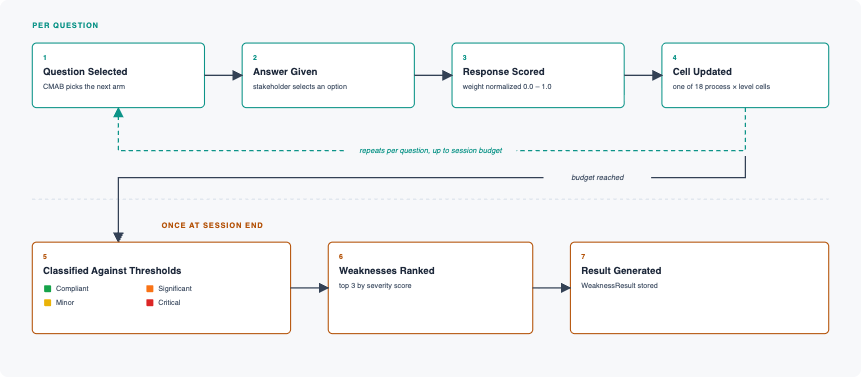
\includegraphics[width=\textwidth]{src/Arch_5.png}
  \caption{Question-to-result processing flow, from question selection to a stored result.
  Generated with Claude Design~\cite{anthropic_claude_design}.}
  \label{fig:question-to-result}
\end{figure}

All 18 scores, together with the top three weaknesses, are written into a single
\texttt{WeaknessResult} row for that session, alongside a timestamp. This is the same write-once
record described in Section~\ref{sec:result-cmab-models}: a final judgement for that session, not
a value that changes afterward. It is also the last step before the stakeholder ever sees a
result -- everything the results dashboard (Section~\ref{sec:user-interface-design}) displays is
read directly from this one row.
\section{API and Interaction Design}
\label{sec:api-design}

Everything mentioned so far -- the question bank, the database, the CMAB engine, the classifier
-- is reached from outside through one thing: a single versioned REST API.

\subsection{API Responsibilities}

The API layer is intentionally kept lightweight. It carries no business logic of its own -- its
routes just validate a request and forward it to the relevant service described earlier in this
chapter. Every endpoint under \texttt{/api/v1} falls into one of three groups: audit session
endpoints, usable by any authenticated stakeholder; question bank endpoints, used by an
administrator to create, edit, and deactivate questions (Section~\ref{sec:answer-weighting}); and
analytics endpoints, giving an administrator aggregate views across every session, feeding the
administration interface (Section~\ref{sec:user-interface-design}).

\subsection{Authentication and Authorization}

Access is JWT-based: the system issues a token when a user logs in, and every subsequent request
carries it. The stakeholder role is collected only once, during signup, as described in
Section~\ref{sec:requirements-analysis}. What separates an ordinary stakeholder from an
administrator is an \texttt{is\_superuser} flag on the user account. Question bank and analytics
endpoints check for this flag explicitly, while audit session endpoints only require a valid
token. This satisfies NFR3 from Section~\ref{sec:requirements-analysis}.

\subsection{Assessment Session Interaction}

Table~\ref{tab:session-endpoints} shows the endpoints a stakeholder uses to join an assessment
session, before they submit any answer.

\begin{table}[h]
\centering
\rowcolors{2}{green!5}{white}
\begin{tabular}{l p{6.5cm}}
\toprule
\rowcolor{green!55!black}
\thw{Endpoint} & \thw{Purpose} \\
\midrule
\texttt{POST /audit/sessions/} & Start a new session; returns the first selected question. \\
\texttt{GET /audit/sessions/} & List the current user's own sessions, past and present. \\
\texttt{GET /audit/sessions/\{id\}} & Retrieve one session's detail, including every question
asked so far. \\
\bottomrule
\end{tabular}
\caption{Assessment session endpoints.}
\label{tab:session-endpoints}
\end{table}

\subsection{Answer Submission and Result Retrieval}

\begin{figure}[h]
  \centering
  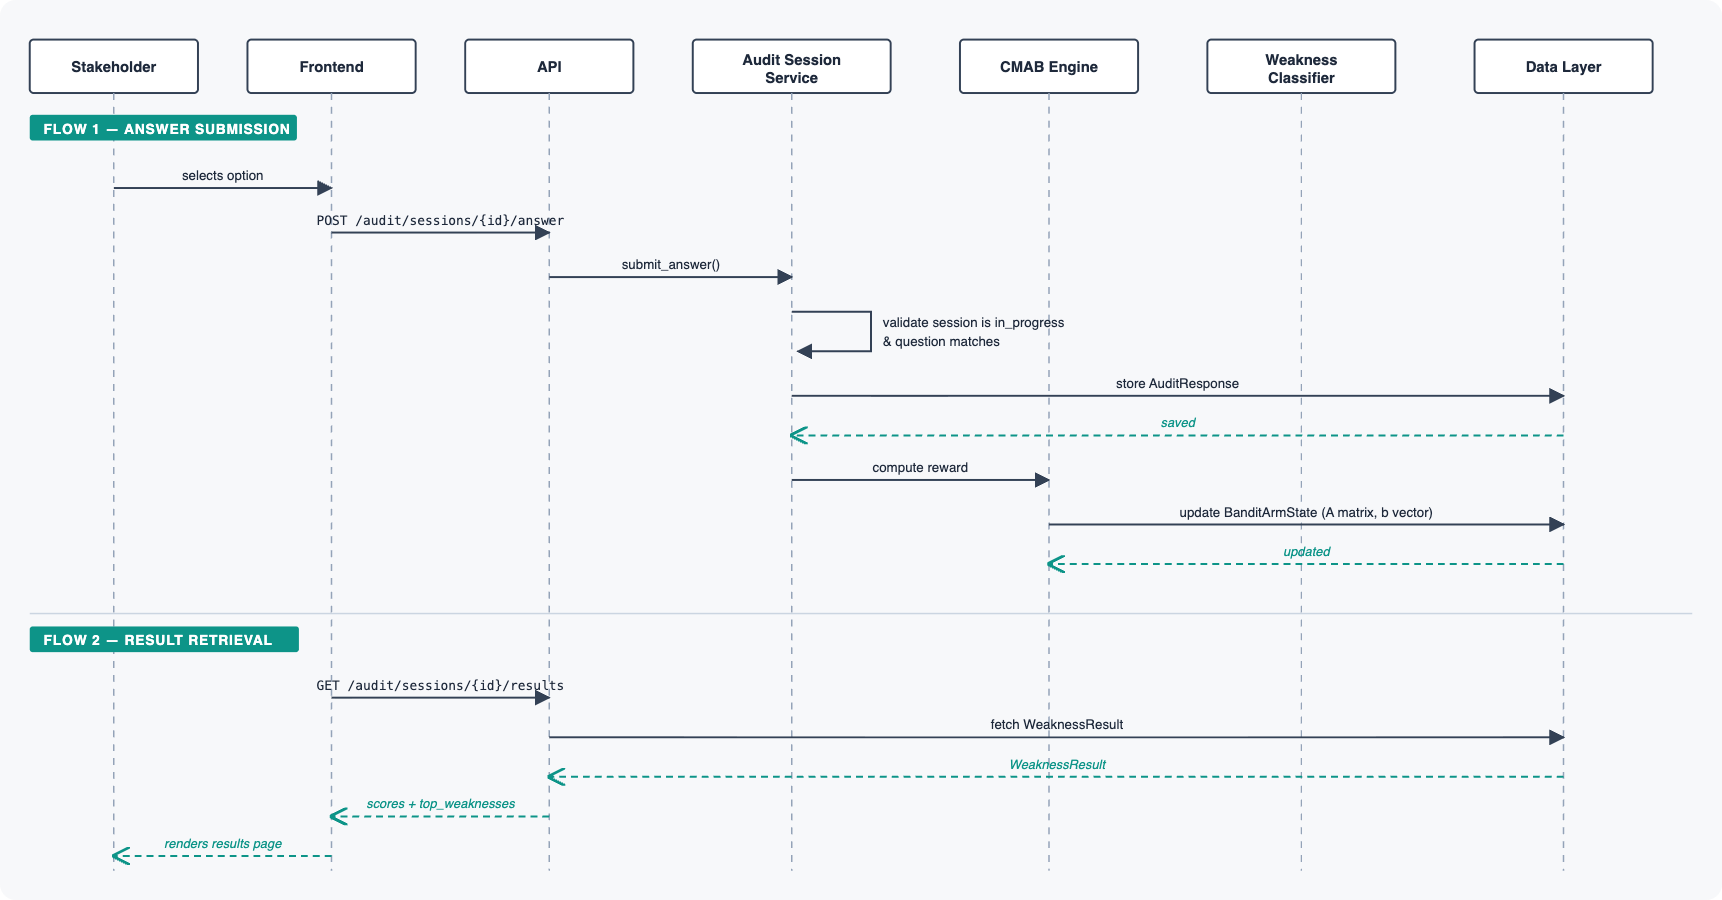
\includegraphics[width=\textwidth]{src/Arch_6_Sequence_diagram.png}
  \caption{Answer submission and result retrieval sequence. Generated with Claude
  Design~\cite{anthropic_claude_design}.}
  \label{fig:arch-answer-sequence}
\end{figure}

Figure~\ref{fig:arch-answer-sequence} shows this interaction from start to finish. Almost the
entire interaction described in Sections~\ref{sec:cmab-engine}
and~\ref{sec:weakness-classification} is carried out by a single answer-submission endpoint. It
first checks that the session is still active and that the question being answered is really the
one the session was waiting for, then it saves the response, computes its reward, and updates
the answered question's \texttt{BanditArmState}. From there, it branches: if the session has not
used up its question budget, it picks and returns the next question; once the budget has been
reached, it runs the classifier, stores the resulting \texttt{WeaknessResult}, and marks the
session completed. A separate results endpoint retrieves that stored result once it exists. This
is useful for the frontend, since a session's result can be requested independently of the
request that produced it -- the client does not need to still be connected at the moment the
session finishes.

\section{User Interface Design}
\label{sec:user-interface-design}

The interface is where every decision made throughout this chapter becomes something a
stakeholder can actually see and interact with, which is why it is organized around the same
role split as the API.

\subsection{User Roles and Views}

There are two types of user, and each is offered a different set of views. Any authenticated
stakeholder sees the views that make up an assessment: starting and taking a session, viewing its
results, and browsing their own session history. An administrator, marked by the same
\texttt{is\_superuser} flag checked at the API level (Section~\ref{sec:api-design}), also gets
access to the question bank manager and the analytics dashboard. The assessment views themselves
do not change for an administrator -- they simply get extra views layered on top.

\subsection{Assessment Session Flow}

A stakeholder never has to wait at an empty screen, since starting a session immediately displays
its first question. Questions are shown one at a time, along with their five possible answers and
a progress indicator (e.g., ``Question 3 of 12''), matching the one-question-at-a-time
interaction described in Section~\ref{sec:api-design}. Once an answer is given, one of two things
happens: the next question picked by the CMAB engine is presented as the current question, or,
once the session's budget is full, the stakeholder is taken straight to their results. The
stakeholder's role is asked only once, at signup, in the same field described in
Section~\ref{sec:requirements-analysis}, and is never asked again.

\subsection{Results Visualization}

A completed session's \texttt{WeaknessResult} (Section~\ref{sec:weakness-classification}) is
displayed in three different ways, each answering a different question. A radar chart, with one
axis per SWE process, gives an instant overview of overall process health. A heatmap table,
processes against capability levels, colours every assessed cell with the same four bands from
Table~\ref{tab:classification-thresholds}, letting a stakeholder see not just how severe a
weakness is, but exactly where it sits. Finally, a ranked list of the top three weaknesses links
each one to the recommendation text carried by the question that revealed it, so the result ends
in more than just a score -- it ends in something actionable.

\subsection{Administration Interface}

Administrators see two additional views, matching the two admin-only endpoint groups from
Section~\ref{sec:api-design}. The question bank manager lists, filters, and directly edits
questions and their options, giving administrators the power to add, edit, and disable questions
in the question bank maintained under FR3 (Section~\ref{sec:requirements-analysis}). The
analytics dashboard is not session-specific but applies across every completed session: it offers
a weakness heatmap for the whole question bank, arm statistics showing which questions are
selected most often and are most rewarding, and participation statistics by stakeholder role. The
difference comes down to the question each view answers: the stakeholder-facing views answer
``How did this session go?'', while the administration view answers ``How is the system behaving
overall?''

\section{Key Design Decisions and Trade-offs}
\subsection{LinUCB versus Alternative Algorithms}

Chapter~\ref{chap:background} introduced four ways to address the exploration--exploitation
dilemma: Epoch-Greedy, $\epsilon$-greedy, Thompson Sampling, and UCB-style methods. This thesis
ultimately uses the contextual member of that group, LinUCB. This subsection puts that decision
on record, and confronts the one piece of evidence that argues against it.

That evidence is not hidden. Table~\ref{tab:recommender-results} in Chapter~\ref{chap:sota},
reproduced from the closest prior work, shows $\epsilon$-greedy outperforming LinUCB on raw reward in
every simulated scenario tested -- by roughly 13 percentage points at a 0\% deficiency-change
rate, narrowing to about 1 point at a 50\% deficiency-change
rate~\cite{datsogiannis2025recommender}. So this is not a choice made because LinUCB is known to
score highest; the choice is based on what this thesis's evaluation actually needs, which is not
quite the same thing as maximizing raw average reward.

Table~\ref{tab:algorithm-comparison} shows the comparison of the four candidates against the
properties relevant to this thesis.

\begin{table}[h]
\centering
\rowcolors{2}{green!5}{white}
\begin{tabular}{l p{4.3cm} c c}
\toprule
\rowcolor{green!55!black}
\thw{Algorithm} & \thw{Selection rule} & \thw{Deterministic?} & \thw{Context-aware?} \\
\midrule
Epoch-Greedy~\cite{langford2007epochgreedy} & Alternates fixed explore/exploit
blocks & Within a block & No \\
$\epsilon$-greedy~\cite{tokic2011valuedifference} & Best known arm, or a
random arm with probability $\epsilon$ & No & No \\
Thompson Sampling~\cite{agrawal2013thompson} & Samples an arm from a fitted
reward distribution & No & Contextual only \\
LinUCB~\cite{li2010contextual,huang2016linucb} & $\theta_a^\top x + \alpha
\sqrt{x^\top A_a^{-1} x}$, highest score wins & Yes & Yes, natively \\
\bottomrule
\end{tabular}
\caption{Bandit algorithms considered, compared on the properties relevant to this thesis.}
\label{tab:algorithm-comparison}
\end{table}

Three reasons, all visible in that table, drove the final choice. First, determinism.
Both $\epsilon$-greedy and Thompson Sampling rely on randomness every single round, either to
choose between exploring and exploiting, or to sample directly from a posterior. That is a
reasonable design for a production system averaging behaviour over millions of rounds, but it is
a problem for a thesis: the same context and model state can legitimately produce a different
next question on a different run, which makes any one session harder to walk through and explain
afterward. LinUCB's score, by contrast, is a deterministic function of $A_a$, $b_a$, and $x$
alone, so a specific session's specific history can always be recomputed and explained, not just
observed.

Second, native context-awareness. Plain $\epsilon$-greedy and plain UCB score an arm
only from its own past average reward -- they have no way to express that a question matters more
to a QA Engineer than to a Project Manager, or that it matters more three questions into a
session than at the start, without bolting on a separate mechanism. LinUCB's scoring rule is
built directly around the 20-dimensional context vector from Section~\ref{sec:cmab-engine}: the
$\theta_a^\top x$ term is not an addition to the algorithm, it is the algorithm. Thompson Sampling
does have contextual variants, but the version benchmarked in Table~\ref{tab:recommender-results}
was not one of them.

Third, one explainable hyperparameter. LinUCB's exploration coefficient $\alpha$ has a
clear, statable meaning: how much weight the uncertainty bonus gets relative to the plain reward
estimate. By comparison, $\epsilon$-greedy's exploration is cruder -- just a fixed or decaying
probability of ignoring the current estimate and exploring randomly -- and Thompson Sampling's
exploration is baked into a fitted distribution that is harder to explain to a reader with no
Bayesian background.

None of this makes $\epsilon$-greedy's simulated result irrelevant. It remains a real result from
the closest prior work, and it shows that LinUCB is not the best-scoring option under pure reward
maximization on simulated data. What it does not tell us is whether that same gap holds up on
real pilot sessions rather than simulated ones -- an evaluation neither prior paper ran. That is
an empirical question this thesis is positioned to actually answer, and
Chapter~\ref{chap:results} addresses it directly.

\section{Chapter Summary}

This chapter turned the requirements from Section~\ref{sec:requirements-analysis} into a
concrete system design: an overall architecture built around a CMAB engine and a weakness
classifier that both sit on the same database, a question bank that maps every question to an
ASPICE base practice, and a REST API and user interface that let stakeholders and administrators
use the system without exposing its internal structure. Where a design decision had a real
alternative, this chapter named it and gave the reasoning behind the choice actually made --
most visibly the decision to use LinUCB despite prior evidence that a simpler algorithm scores
higher in simulation. Chapter~\ref{chap:implementation} now turns this design into running code.

\chapter{Implementation}
\label{chap:implementation}
% \input{src/implementation}

The design of Chapter~\ref{chap:architecture} turns into running code in this chapter. It starts
with the development environment and tooling used to build the system, then works its way
through the backend implementation, the question bank, and the frontend. It also covers
deployment and runtime configuration, and concludes with the implementation issues that arose
and how they were addressed.

\section{Development Environment and Tooling}

This section covers the tools the system was actually built with, before the rest of the chapter
turns to the implementation itself. It starts with how development and production are kept in
sync through containerization, then covers the backend stack built around FastAPI and SQLModel,
and finally the frontend stack built around React and a generated API client.

\subsection{Containerized Development Environment}

The entire system is deployed in Docker containers, in both development and production, so that
a configuration verified on one machine behaves identically on any other, eliminating the common
discrepancy between a developer's machine and the deployed environment. This is done locally
using \texttt{compose.yml} and a For development, create a \texttt{compose.override.yml} file to
replace a few of the above: The ports of database and admin GUI are exposed directly to the
host. The backend and the frontend are running with a live-reloading, of course, and sitting
behind Traefik. Use setup instead of built production image.

At the service level, the React frontend communicates with the FastAPI backend over REST/JSON,
and the backend communicates with PostgreSQL via SQLAlchemy's ORM. Docker Compose puts all three
on the same network, gives the database a persistent volume, and enforces a start order of
\texttt{web} $\to$ \texttt{api} $\to$ \texttt{db}. Each container exposes its own internal port;
locally, Adminer sits alongside these three, and the ports actually exposed on the host are the
ones listed below.

Four services make up the stack: PostgreSQL (\texttt{db}, port 5433 locally), the FastAPI The
Vite dev server (\texttt{frontend}, port 5173), Ad- For direct access to the database during
development, use miner (\texttt{adminer}, port 8080) to poke at the database directly. When
running \texttt{docker compose watch}, all four will be run with live reloading enabled, so a
change in either the backend or the frontend shows up in the browser within a second or two,
without ever having to restart manually.

\subsection{Backend Development Stack}

\begin{figure}[h]
  \centering
  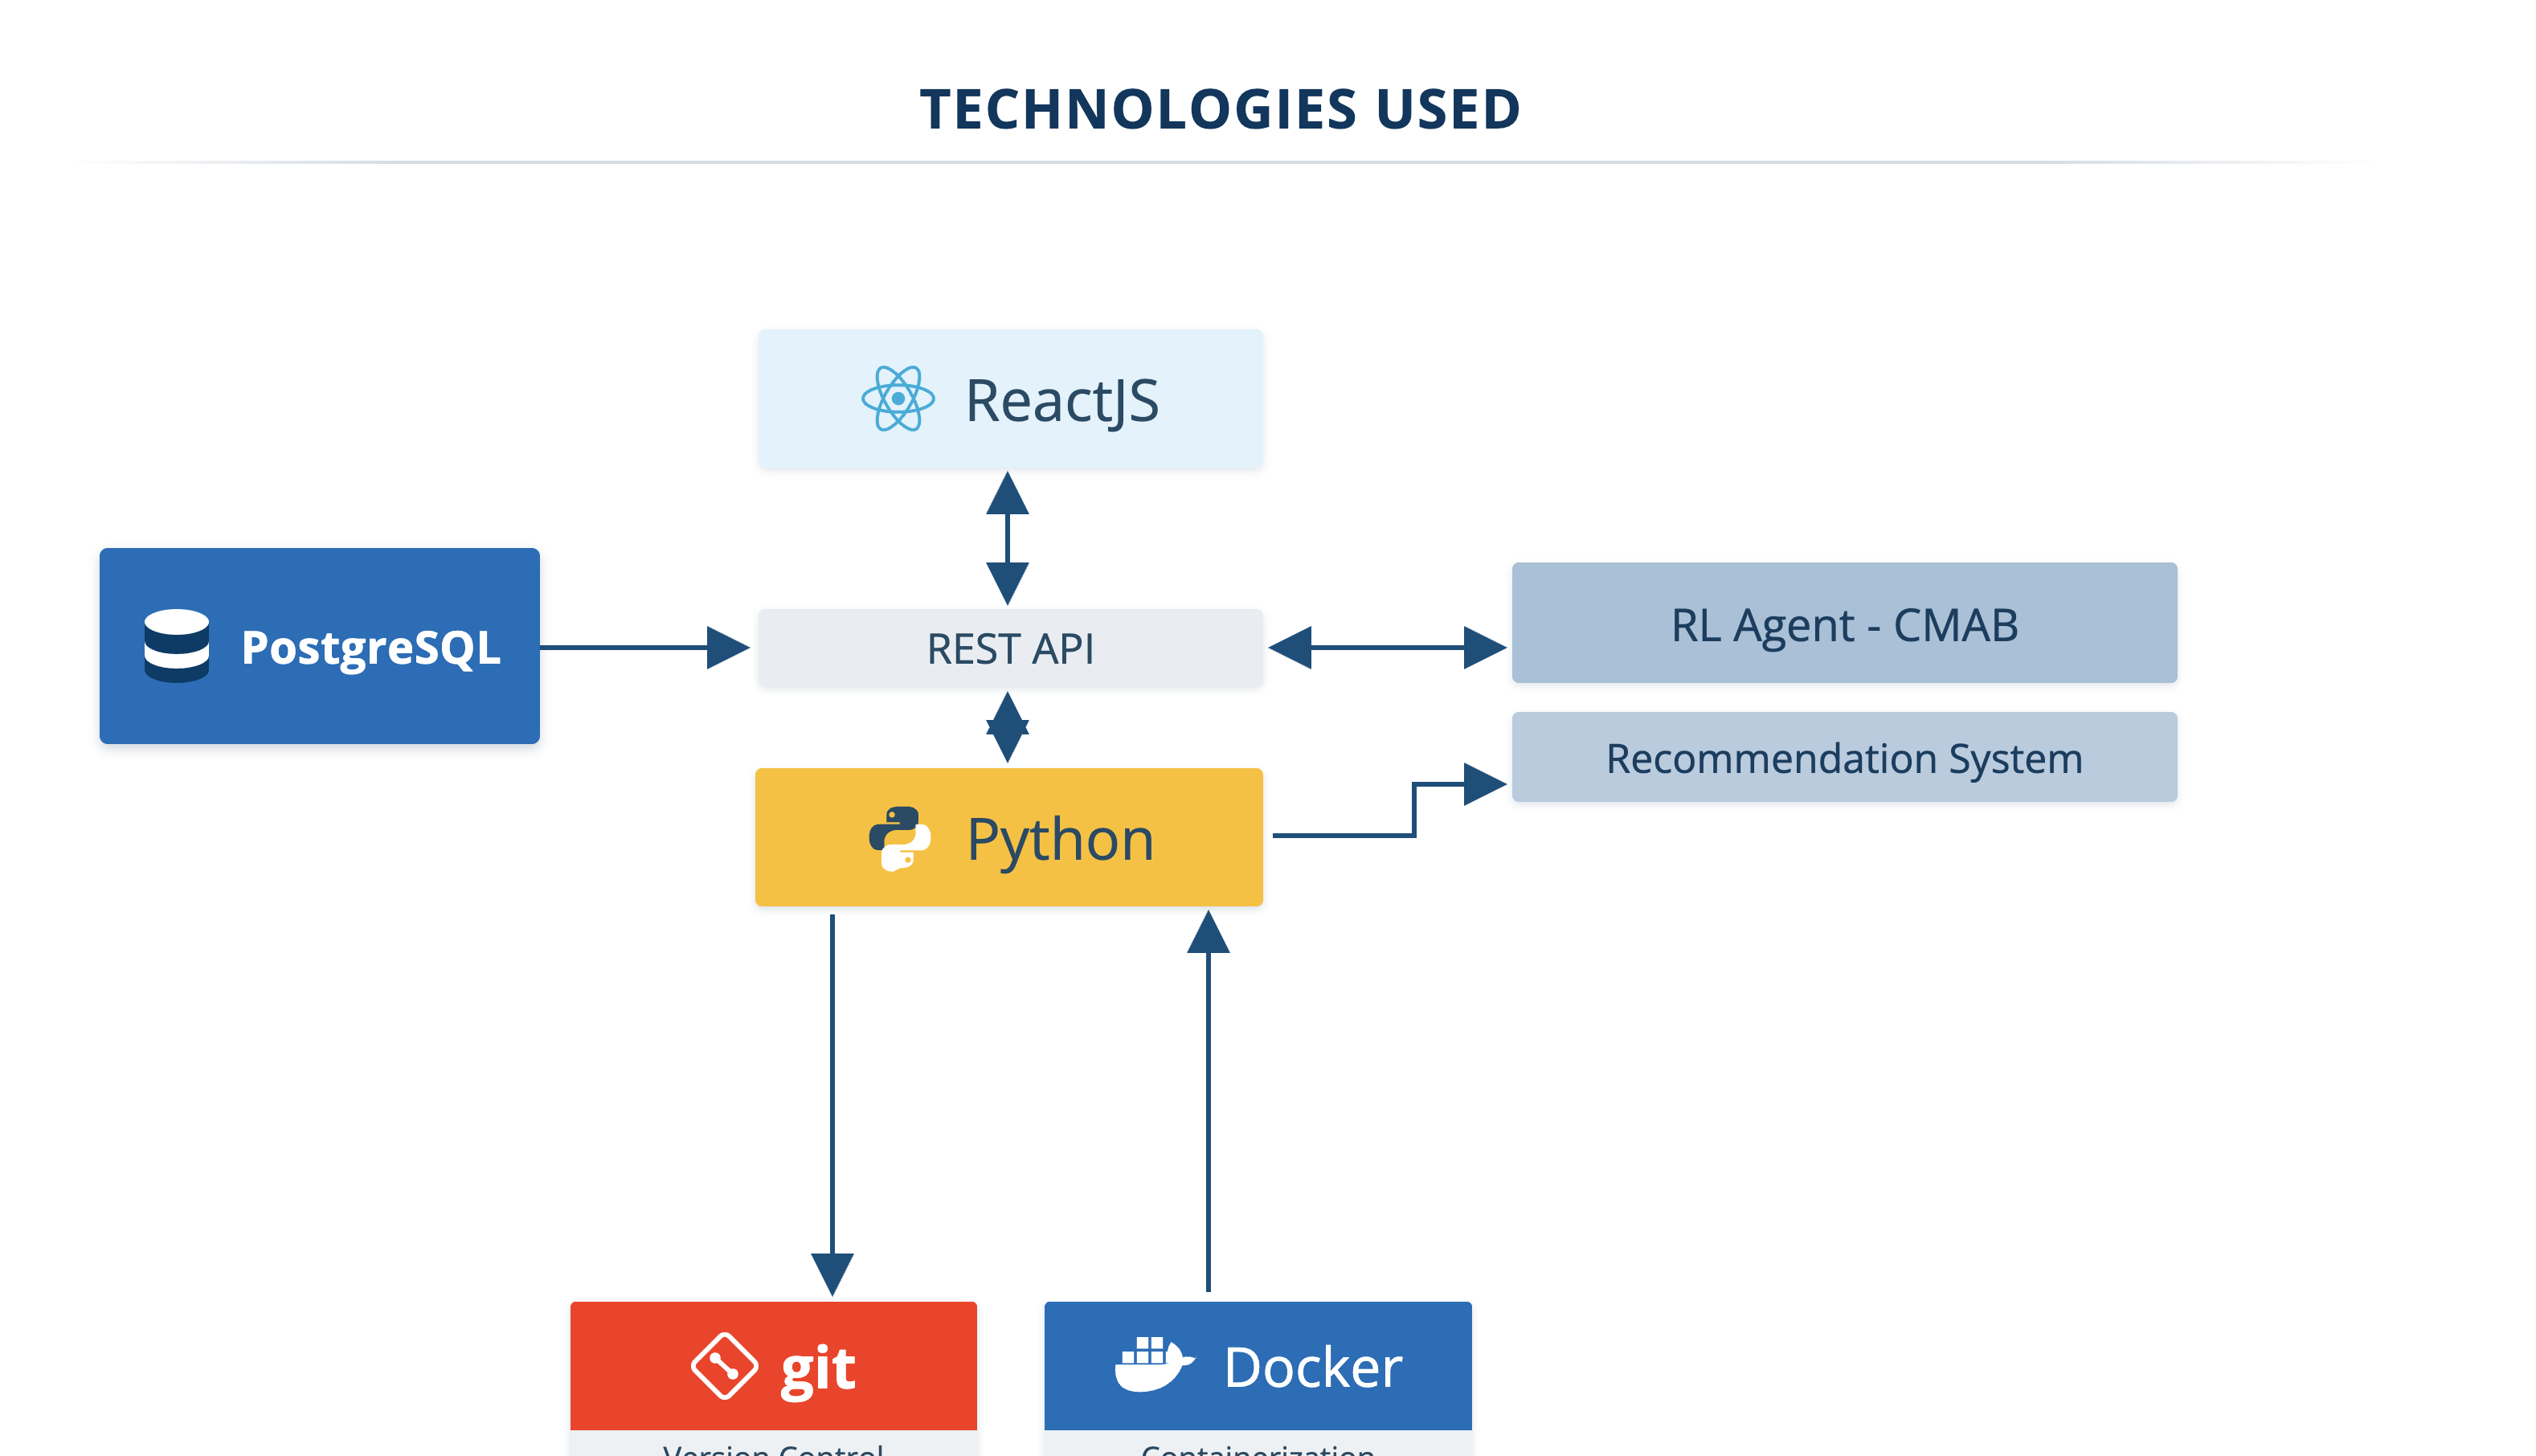
\includegraphics[width=\textwidth]{src/Imp_backend_2.png}
  \caption{Technologies used across the stack. Generated with Claude Design~\cite{anthropic_claude_design}.}
  \label{fig:tech-stack}
\end{figure}

The backend is created using FastAPI, an async web framework. Validates all requests and
responses against a Pydantic model, and generates the model from the response. The typed client
that the frontend is built from, based on OpenAPI schema.

On top of that, SQLModel is directly on top of that: one model class is the same thing as two.
SQLAlchemy table definition and the Pydantic schema FastAPI validates against, A table such as
\texttt{AuditQuestion} needs only to be defined once, so a table like that is not a suitable
candidate for a table function.

\texttt{uv} is the package manager, both locally and in the backend's Dockerfile, with One
\texttt{uv.lock} file containing all the exact versions of all the dependencies. Alembic handles
schema migrations: every change to a SQLModel table, such as adding \texttt{stakeholder\_role} to
\texttt{User}, or creating the tables described in Chapter~\ref{chap:architecture}, is captured
as its own A script that can be run in both directions, and is versioned.

\subsection{Frontend Development Stack}

\begin{figure}[h]
  \centering
  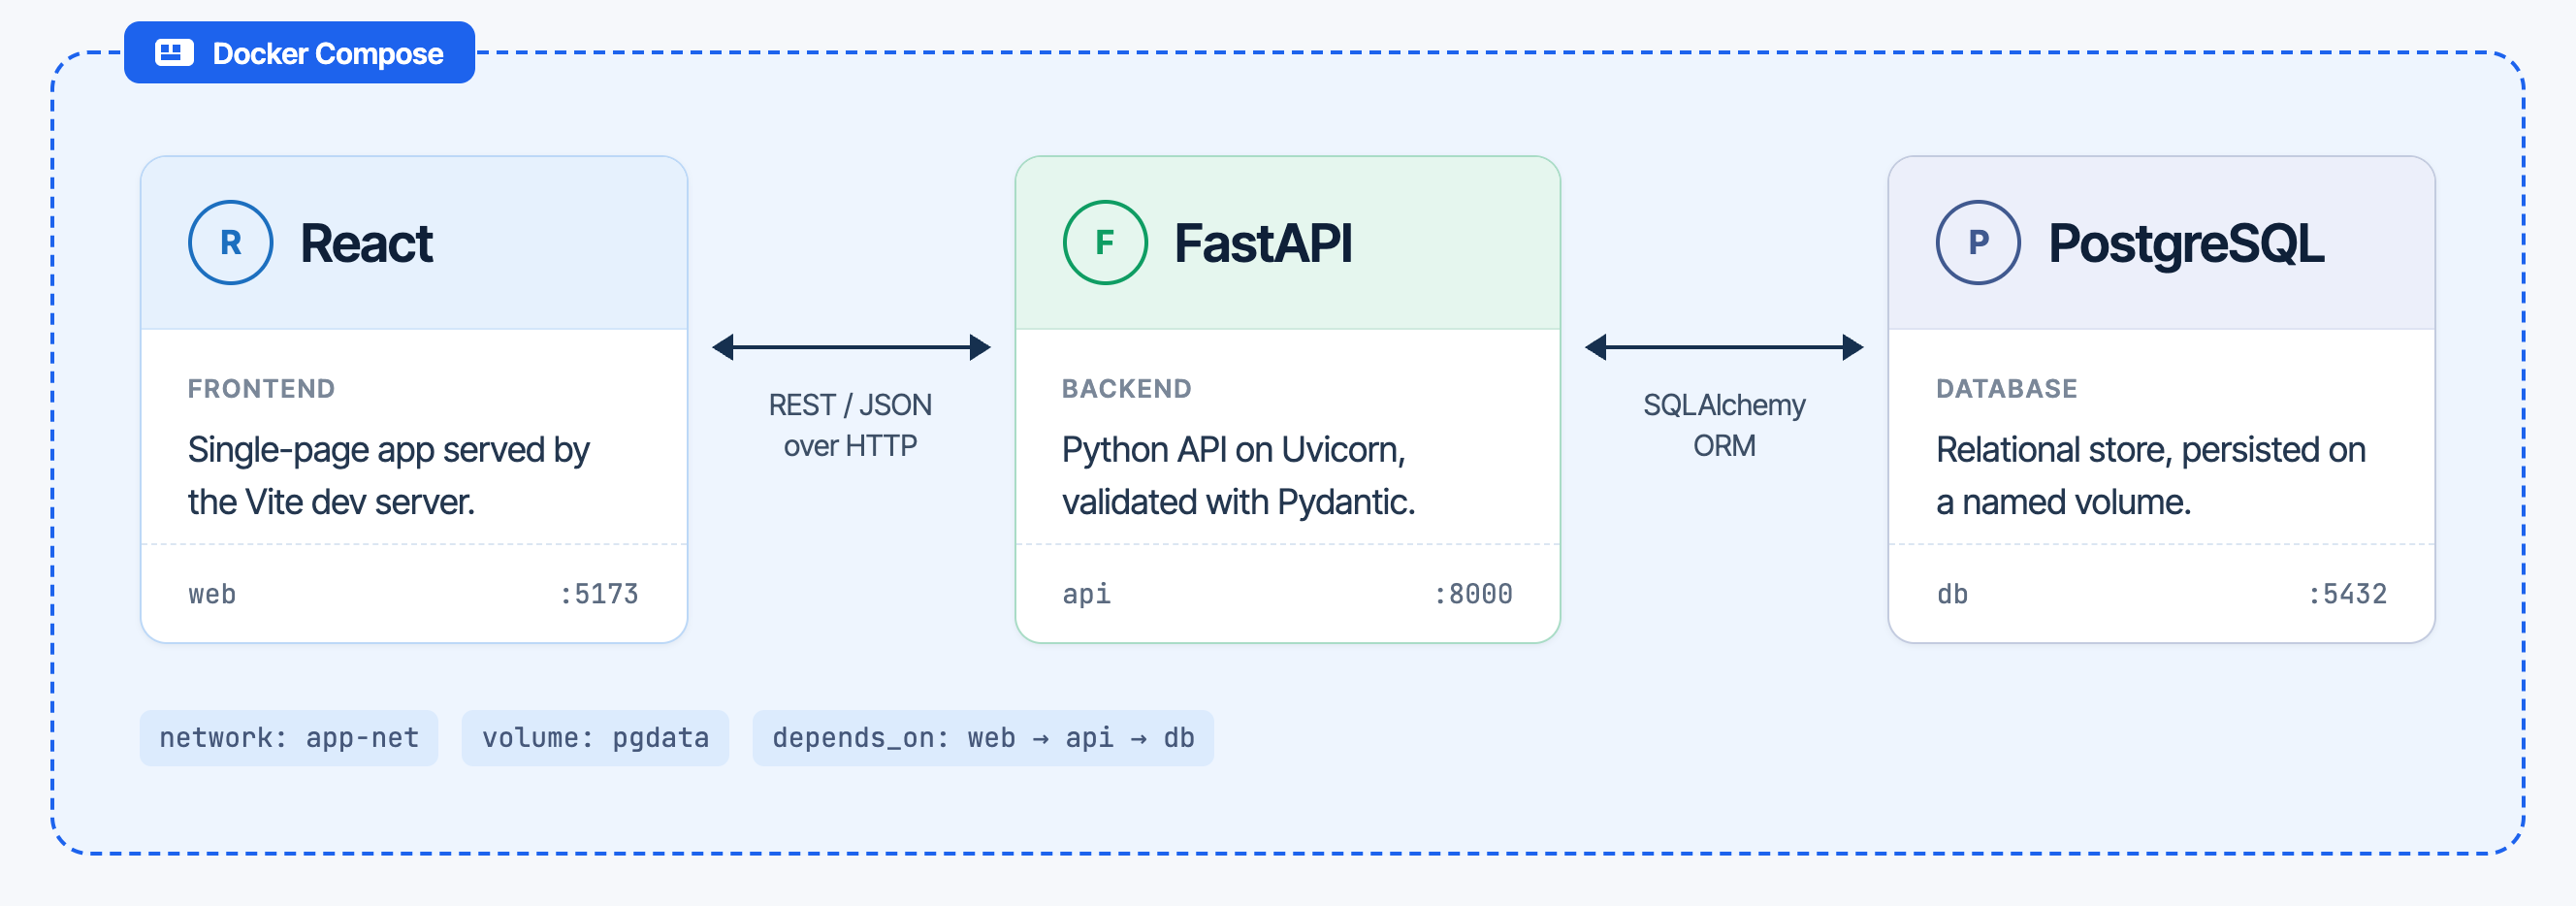
\includegraphics[width=\textwidth]{src/Imp_frontend_3.png}
  \caption{Frontend development stack and data flow. Generated with Claude
  Design~\cite{anthropic_claude_design}.}
  \label{fig:frontend-stack}
\end{figure}

The frontend is made with React and TypeScript, built and served in dev with Vite, fast enough
to see a saved file almost instantly in the browser. TanStack Router is responsible for routing,
and the route tree is created based on the file structure in TanStack Query manages server state
(caching, refetching, and loading and error states) for every API call.

The API client is generated, not hand-written: \texttt{openapi-ts} generates a A fully typed
TypeScript client directly from the OpenAPI schema of the backend, so a If the shape of the
request or the response does not match, it will be reported as a type error at build time. than
a runtime bug.

\section{Backend Implementation}
\subsection{Backend Project Structure}

The backend follows a layered structure, matching the API Responsibilities split introduced in
Chapter~\ref{chap:architecture}: routes stay thin, and the real logic lives in a separate
\texttt{services} package.

\begin{verbatim}
backend/app/
|-- services/
|   |-- audit_service.py        # session start/answer/complete workflow
|   |-- cmab_engine.py          # LinUCB: context, selection, update
|   `-- weakness_classifier.py  # scoring, thresholds, top weaknesses
|-- api/
|   |-- main.py                 # router registration
|   |-- deps.py                 # auth + DB session dependencies
|   `-- routes/
|       |-- audit.py            # /audit/sessions/* endpoints
|       |-- questions.py        # /questions/* endpoints (admin)
|       |-- analytics.py        # /analytics/* endpoints (admin)
|       `-- users.py, login.py  # existing auth endpoints
|-- core/                       # config.py, db.py, security.py
|-- models.py                   # SQLModel tables + Pydantic schemas
|-- crud.py                     # DB helper functions
`-- seed_questions.py           # question bank seeding script
\end{verbatim}

A route handler never touches the database directly or runs any CMAB math itself, it validates
the request, calls into \texttt{audit\_service}, \texttt{cmab\_engine}, or
\texttt{weakness\_classifier}, and returns whatever that service gives back. This is what keeps
the three services testable on their own, independent of FastAPI or HTTP entirely.

\subsection{Data Models and Database Migrations}

The data model from Chapter~\ref{chap:architecture} is implemented as one set of table
definitions that also serve as the API's request and response schemas, so each entity is
declared once instead of being kept in step across two layers. The existing \texttt{User}
entity gains a single \texttt{stakeholder\_role} attribute. Six assessment entities are added
alongside it, all shown in Figure~\ref{fig:erd}: \texttt{AuditQuestion}, \texttt{AuditOption},
\texttt{AuditSession}, \texttt{AuditResponse}, \texttt{WeaknessResult}, and
\texttt{BanditArmState}.

Primary keys are chosen to match how each entity is used. Reference data that an administrator
manages, namely users, questions, and options, keeps sequential integer keys. The four
session-scoped entities are written concurrently by many stakeholders at once and use UUIDs
instead, so parallel sessions never contend over a shared counter. Every schema change is
recorded as a versioned migration that can be applied or reversed, keeping all environments on
the same database structure.

\subsection{Audit Session Service}

A single coordinating component owns the lifecycle of an assessment session and is the only
place where the recommendation engine and the weakness classifier meet. Starting a session
creates the session record, assembles the first context vector, and requests an opening
question from the engine.

Each answer is then handled in a fixed order: it is checked against the question the session is
actually waiting for, stored, converted into a reward, and used to update that question's
learned state. The component then decides whether the session goes on or stops. It stops when
the question budget is used up or when no eligible questions are left; otherwise the context is
rebuilt and the engine is asked for the next question. Once a session stops, the classifier
runs, its result is saved, and the session is marked complete. This is the flow already drawn
in Figure~\ref{fig:arch-answer-sequence}.

At present the eligibility check is narrower than the design in Chapter~\ref{chap:architecture}.
It drops questions that are inactive or already asked, but does not yet drop questions outside
the stakeholder's role; role still enters through the context vector, so it changes which
question ranks highest rather than which questions are eligible at all. Making role a hard
filter is an isolated change left for future work.


\subsection{CMAB Engine Implementation}

The engine implements the LinUCB rule from Chapter~\ref{chap:architecture} using ordinary
matrix and vector arithmetic. Before each question it builds the 20-dimensional context vector
of Table~\ref{tab:context-vector} from the stakeholder's role and the current state of the
session.

For every eligible question it retrieves the two quantities LinUCB keeps per arm: a matrix
$A_a$ and a vector $b_a$ that together summarise what has been learned about that question, or
an identity matrix and a zero vector if the question has never been asked. It then forms
$\theta_a = A_a^{-1} b_a$ and scores the question by adding its predicted reward
$\theta_a^\top x$ to an uncertainty bonus. The highest-scoring question is returned. After the
answer, the chosen option's weight is normalised into a reward, a fixed bonus is added when the
question is the first from its process in that session, and the reward is folded back into
$A_a$ and $b_a$ with one rank-one update. The updated values are stored as JSON, so the learned
state persists between requests without a separate numeric store.

\begin{table}[h]
\centering
\rowcolors{2}{green!5}{white}
\begin{tabular}{c p{4.3cm} p{6.2cm}}
\toprule
\rowcolor{green!55!black}
\thw{Dims} & \thw{Content} & \thw{How computed} \\
\midrule
0--6 & Stakeholder role (one-hot) & 1.0 at the user's role position, 0 elsewhere \\
7 & Session progress & \texttt{questions\_asked / max\_questions} (0.0 to 1.0) \\
8--13 & Per-process coverage flags (SWE1 to SWE6) & 1.0 if at least one question from that
process was already asked \\
14--19 & Running mean weakness score per process & Average of normalised answer weights for
each process so far \\
\bottomrule
\end{tabular}
\caption{The 20-dimensional context vector built before each question.}
\label{tab:context-vector}
\end{table}


\subsection{Weakness Classifier Implementation}

Turning a finished session into a result is deliberately simple. Each answer contributes the
normalised weight of its chosen option. These values are grouped by the (process, capability
level) pair of the question they came from and averaged within each group, giving one score per
assessed cell of the process-by-level grid; pairs the session never covered are left empty
rather than scored as zero. Every score is placed in one of the four bands from
Table~\ref{tab:classification-thresholds}, and the assessed cells are ranked so the three worst
can be reported with their recommendations, as in Figure~\ref{fig:question-to-result}.


\subsection{API Routes and Dependency Injection}

Every route is kept thin. It resolves a small set of shared dependencies, calls one service,
and returns what the service produces. Three dependencies cover the common needs: one opens a
database session for the request and releases it afterwards, one reads the bearer token,
validates it, and loads the current user, and a third builds on that user and additionally
requires an administrator account, guarding the question bank and analytics routes.

The routes are grouped by concern and mounted under a single versioned prefix,
\texttt{/api/v1}: the audit session routes, the question bank routes, the analytics routes, and
the authentication and user routes carried over from the project template. From these groups
the framework generates an OpenAPI description and serves it as interactive documentation.
Figures~\ref{fig:be-api-audit} to~\ref{fig:be-api-analytics} show the three assessment-facing
groups as they appear in that documentation.

\begin{figure}[h]
  \centering
  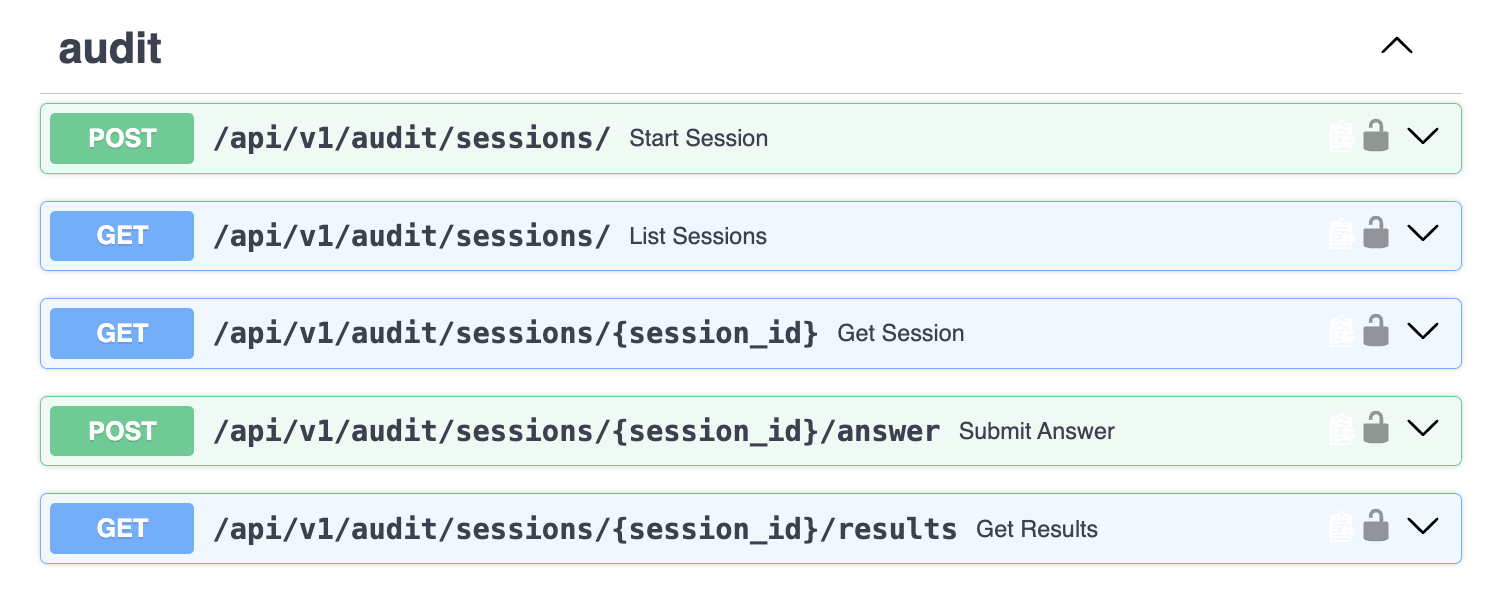
\includegraphics[width=\textwidth]{src/Imp_backend_audit_12.png}
  \caption{The \texttt{audit} router in the generated OpenAPI documentation.}
  \label{fig:be-api-audit}
\end{figure}

Chapter~\ref{chap:architecture} already tabulates the three session endpoints;
Table~\ref{tab:admin-endpoints} lists the admin-only ones.

\begin{table}[h]
\centering
\rowcolors{2}{green!5}{white}
\begin{tabular}{l p{6.5cm}}
\toprule
\rowcolor{green!55!black}
\thw{Endpoint} & \thw{Purpose} \\
\midrule
\texttt{GET /questions/} & List questions (filters: process, level, role, is\_active) \\
\texttt{POST /questions/} & Create a question with its options \\
\texttt{PATCH /questions/\{id\}} & Edit a question or its options \\
\texttt{DELETE /questions/\{id\}} & Deactivate a question (soft delete) \\
\texttt{POST /questions/seed} & Bulk-seed questions from a JSON payload \\
\texttt{GET /analytics/weaknesses} & Aggregate weakness scores across all sessions \\
\texttt{GET /analytics/users} & Participation stats by stakeholder role \\
\texttt{GET /analytics/bandit} & CMAB arm stats: pull count, average reward per question \\
\bottomrule
\end{tabular}
\caption{Question bank and analytics endpoints (admin only).}
\label{tab:admin-endpoints}
\end{table}

\begin{figure}[h]
  \centering
  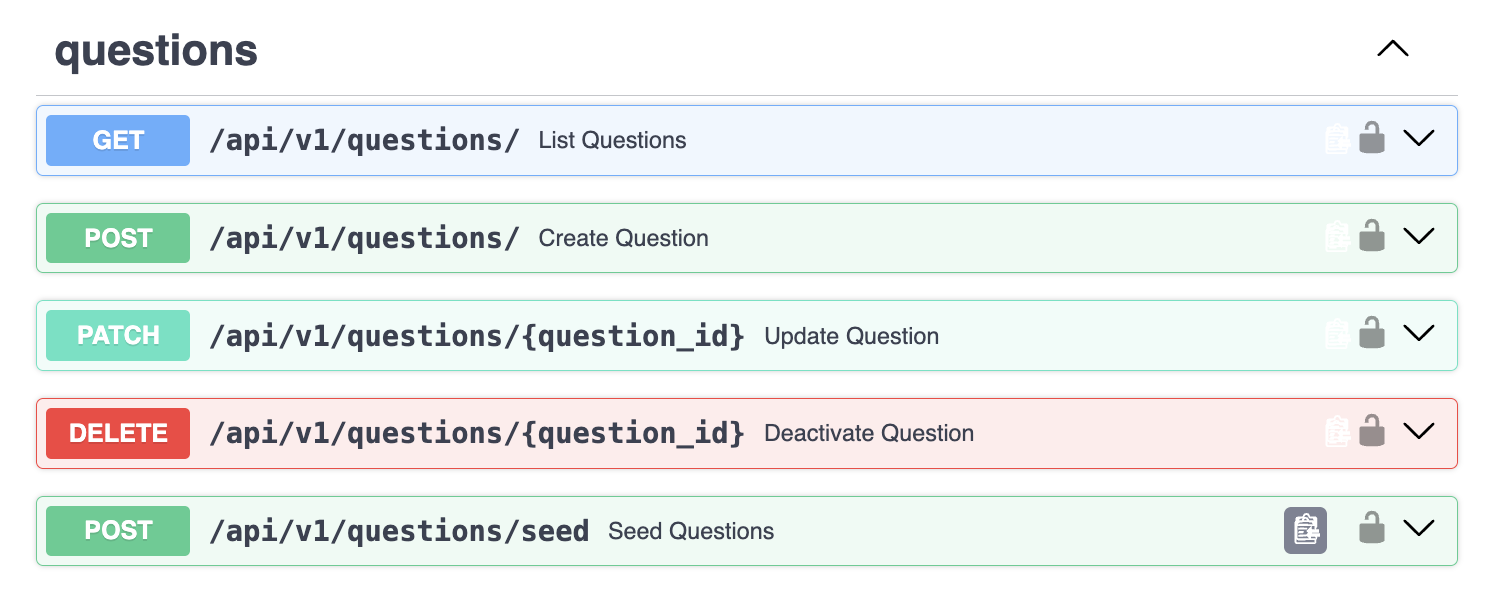
\includegraphics[width=\textwidth]{src/Imp_backend_questions_13.png}
  \caption{The \texttt{questions} router in the generated OpenAPI documentation (superuser-only).}
  \label{fig:be-api-questions}
\end{figure}

\begin{figure}[h]
  \centering
  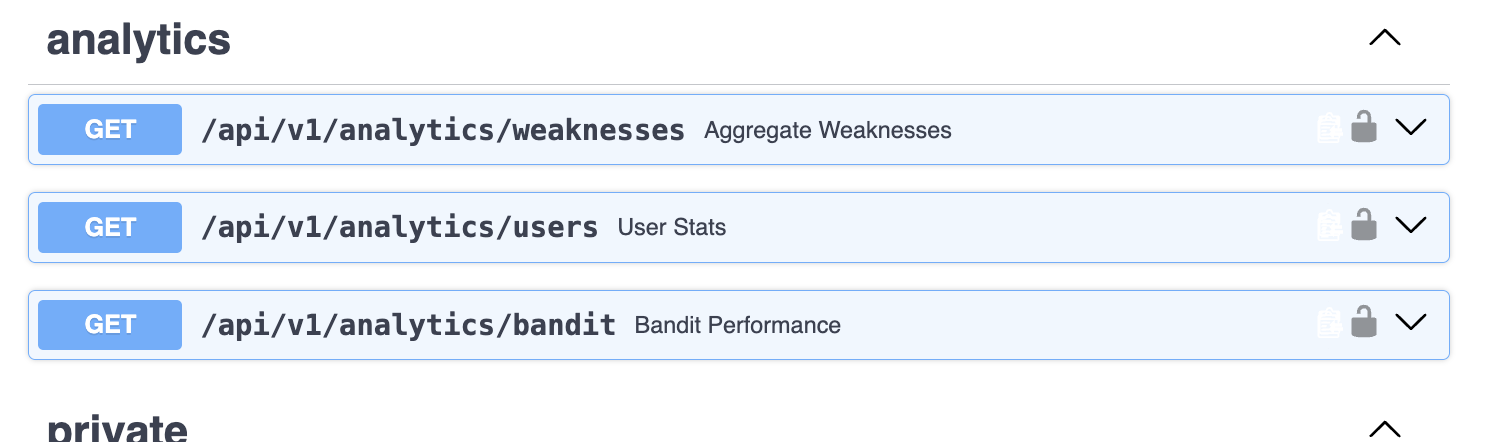
\includegraphics[width=\textwidth]{src/Imp_backend_analytics_14.png}
  \caption{The \texttt{analytics} router in the generated OpenAPI documentation (superuser-only).}
  \label{fig:be-api-analytics}
\end{figure}

\subsection{Authentication and Authorization}

Every protected route depends on \texttt{CurrentUser} from \texttt{deps.py}, which decodes the
bearer token, looks up the matching \texttt{User}, and rejects the request if that user is
inactive or the token does not validate. Question-bank and analytics routes add
\texttt{get\_current\_active\_superuser} on top, so only an account with \texttt{is\_superuser}
set can reach them; audit session routes only require a valid token, plus an explicit ownership
check so one stakeholder cannot read another's session by guessing its ID. Signup collects
\texttt{stakeholder\_role} as part of the existing registration payload, stored on the
\texttt{User} row from that point on, exactly as described in Chapter~\ref{chap:architecture}.
The \texttt{login} and \texttt{users} routers carried over from the project template
(Figures~\ref{fig:be-api-login} and~\ref{fig:be-api-users}) provide token issue, password
recovery, and user management; \texttt{POST /users/signup} is the one public write, and it is
where \texttt{stakeholder\_role} first enters the system.

\begin{figure}[h]
  \centering
  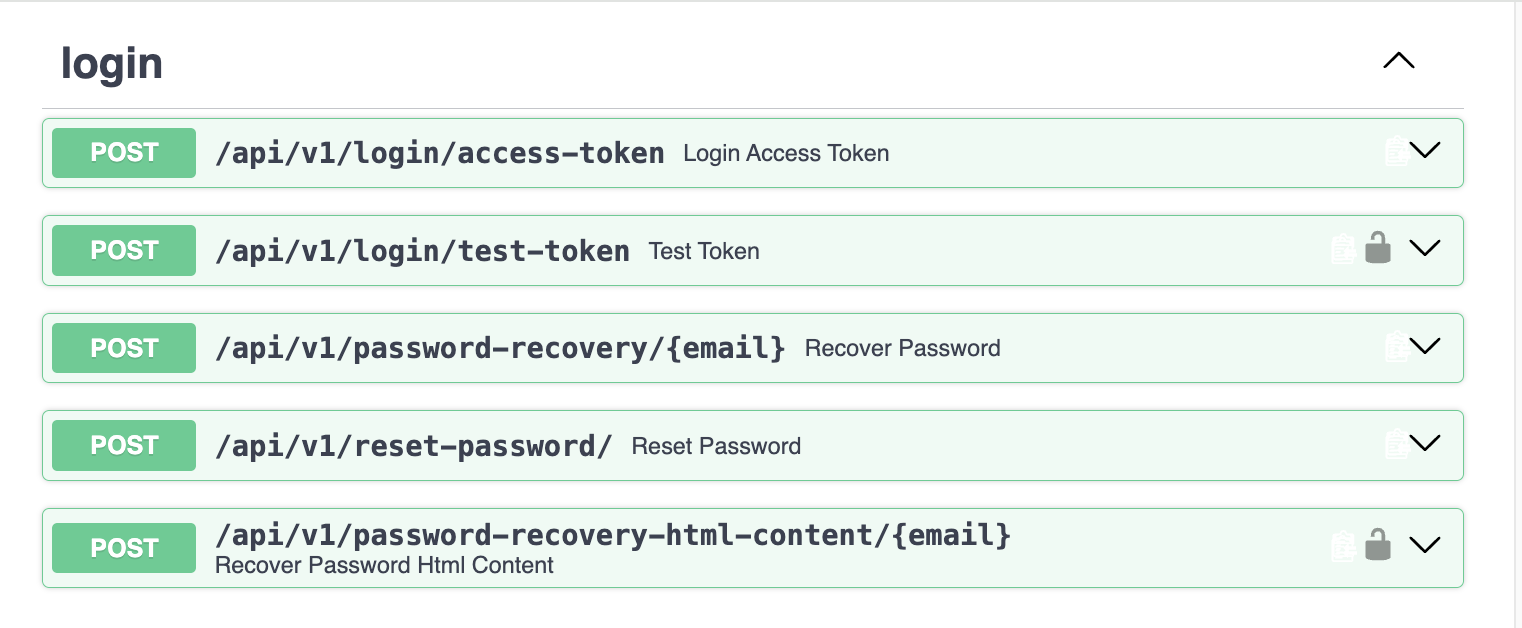
\includegraphics[width=\textwidth]{src/Imp_backend_login_10.png}
  \caption{The \texttt{login} router in the generated OpenAPI documentation.}
  \label{fig:be-api-login}
\end{figure}

\begin{figure}[h]
  \centering
  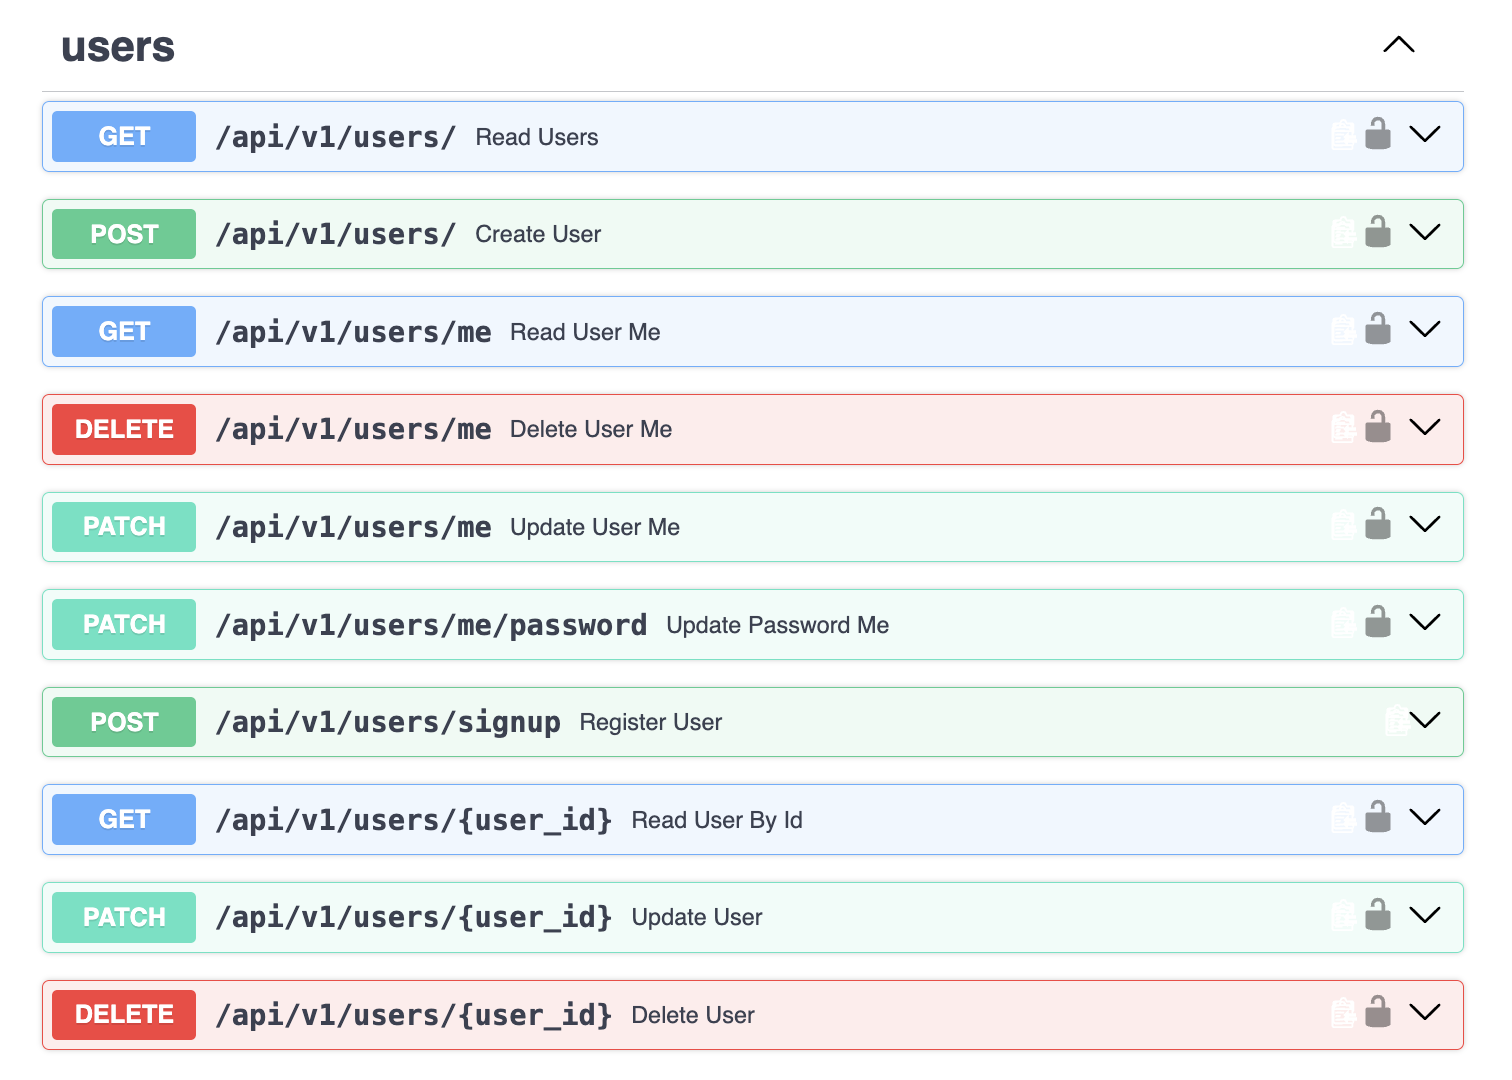
\includegraphics[width=\textwidth]{src/Imp_backend_user_11.png}
  \caption{The \texttt{users} router in the generated OpenAPI documentation.}
  \label{fig:be-api-users}
\end{figure}

\section{Question Bank Implementation}
\label{sec:question-bank-impl}

\subsection{Question Bank Data Preparation}

The question bank was authored directly from the SWE.1--SWE.6 base practices in the
PAM~\cite{vdaqmc2023pam}, following the transformation set out in
Chapter~\ref{chap:architecture}. Each base practice was read the way an assessor would read it,
then rephrased as a single question a stakeholder can answer about work that already exists,
with the practice's detailed criteria pushed down into the wording of the answer options rather
than repeated in the question text. The result is ten questions per process and 60 in total,
each with five options (A--E) carrying weights $0$--$5$, for 300 options overall; the full list
is given in Appendix~\ref{app:questionbank}.

Coverage was checked per process rather than left to chance. Every SWE process contributes the
same number of questions, and within a process the questions are spread across that process's
base practices so no single practice is over- or under-represented. Table~\ref{tab:qb-counts}
lists the totals.

\begin{table}[h]
\centering
\rowcolors{2}{green!5}{white}
\begin{tabular}{l c}
\toprule
\rowcolor{green!55!black}
\thw{Item} & \thw{Count} \\
\midrule
SWE processes covered (SWE.1--SWE.6) & 6 \\
Questions per process & 10 \\
Questions in total & 60 \\
Answer options per question (A--E) & 5 \\
Answer options in total & 300 \\
\bottomrule
\end{tabular}
\caption{Seeded question bank totals.}
\label{tab:qb-counts}
\end{table}

\subsection{Seed Script and Idempotent Seeding}

The authored bank lives in \texttt{seed\_questions.py} as a static list of question records,
each carrying its code, process, base-practice ID, text, recommendation, stakeholder roles, and
its five weighted options. Loading it is a single step: the script opens one database session,
iterates the list, and for each record looks up the existing \texttt{AuditQuestion} by its
\texttt{question\_code}. A question that is not present is inserted together with its options; a
question that is already there has its editable fields refreshed in place and its options
matched by letter and updated. Nothing is deleted. Because every write is keyed on
\texttt{question\_code}, the script is idempotent: running it against an empty database
populates the bank, and running it again after an edit reconciles the rows without creating
duplicates. It is invoked once on first startup and re-run by hand whenever the source list
changes.

\subsection{Traceability and Stakeholder Role Fields}

Two fields on \texttt{AuditQuestion} carry the requirements established in
Chapter~\ref{chap:architecture} down to the implementation. \texttt{base\_practice\_id} stores
the PAM identifier each question was derived from (\texttt{SWE.1.BP1} for
\texttt{SWE1\_L1\_01}, and so on), so that a question's justification against the standard is a
single lookup away; this is what satisfies NFR2 from Section~\ref{sec:requirements-analysis}.
The \texttt{stakeholders} field holds the list of roles a question applies to, drawn from the
seven roles defined in Chapter~\ref{chap:architecture}. At the start of a session and after
every answer, the eligibility filter in \texttt{audit\_service.py} keeps only those questions
whose \texttt{stakeholders} list contains the current user's \texttt{stakeholder\_role} and
that have not yet been asked; the questions that survive the filter are the arms handed to the
CMAB engine (Section~\ref{sec:cmab-engine}). Neither field is ever shown to the stakeholder;
both exist purely to keep each question traceable to the standard and targeted at the right
roles.

\section{Frontend Implementation}
\label{sec:frontend-impl}

\subsection{Frontend Project Structure and Routing}

The frontend is a single-page React application. Routing is handled by TanStack Router in
file-based mode: every file under \texttt{frontend/src/routes} is a route, and the router plugin
regenerates a typed \texttt{routeTree.gen.ts} on every save, so paths and their parameters are
checked at compile time. The routes fall into two groups. \texttt{login}, \texttt{signup}, and
the password-recovery routes render on their own, with no application chrome. Everything else is
nested under a \texttt{\_layout} route whose \texttt{beforeLoad} hook redirects to
\texttt{/login} unless an access token is present. This single guard is what makes every
assessment and administration page private, rather than a check repeated on each page. The
authenticated shell it renders is a sidebar, a header, and an \texttt{<Outlet>} for the active
page. Server data on every page is fetched and cached through TanStack Query, so navigation
between pages reuses data already loaded rather than refetching it.

Table~\ref{tab:frontend-routes} lists the pages a stakeholder moves through during an
assessment. The two session routes take the session ID as a path parameter
(\texttt{/audit/:sessionId} and \texttt{/audit/:sessionId/results}) and additionally check that
the session belongs to the current user, so one stakeholder cannot open another's session or
results by editing the URL.

\begin{table}[h]
\centering
\rowcolors{2}{green!5}{white}
\begin{tabular}{l l}
\toprule
\rowcolor{green!55!black}
\thw{Page} & \thw{Access} \\
\midrule
Sign-up and login & Public \\
Audit list and assessment home & Authenticated \\
Audit session (one question at a time) & Session owner \\
Audit results & Session owner \\
Audit history & Authenticated \\
Question bank manager & Administrator \\
Analytics dashboard & Administrator \\
User administration & Administrator \\
\bottomrule
\end{tabular}
\caption{Main frontend pages and who can reach them.}
\label{tab:frontend-routes}
\end{table}

\subsection{Authentication and User Management}

Authentication state lives entirely in the browser. The \texttt{useAuth} hook treats the
presence of an \texttt{access\_token} key in \texttt{localStorage} as ``logged in''; the login
mutation posts the e-mail and password to the token endpoint from
Section~\ref{sec:api-design}, stores the returned bearer token, and the generated API client
attaches it to every subsequent request. Logout clears the key and the cached queries.

The signup form (Figure~\ref{fig:fe-signup}) is a \texttt{react-hook-form} form validated
against a \texttt{zod} schema. Alongside e-mail and password it carries one assessment-specific
field: a \texttt{stakeholder\_role} dropdown backed by the seven roles from
Chapter~\ref{chap:architecture}. The schema also enforces a password-confirmation match, and
the confirmation field is stripped from the payload before it is sent. This is the only place
in the application where a role is chosen, matching the ``asked once'' rule from
Section~\ref{sec:requirements-analysis}.

\begin{figure}[h]
  \centering
  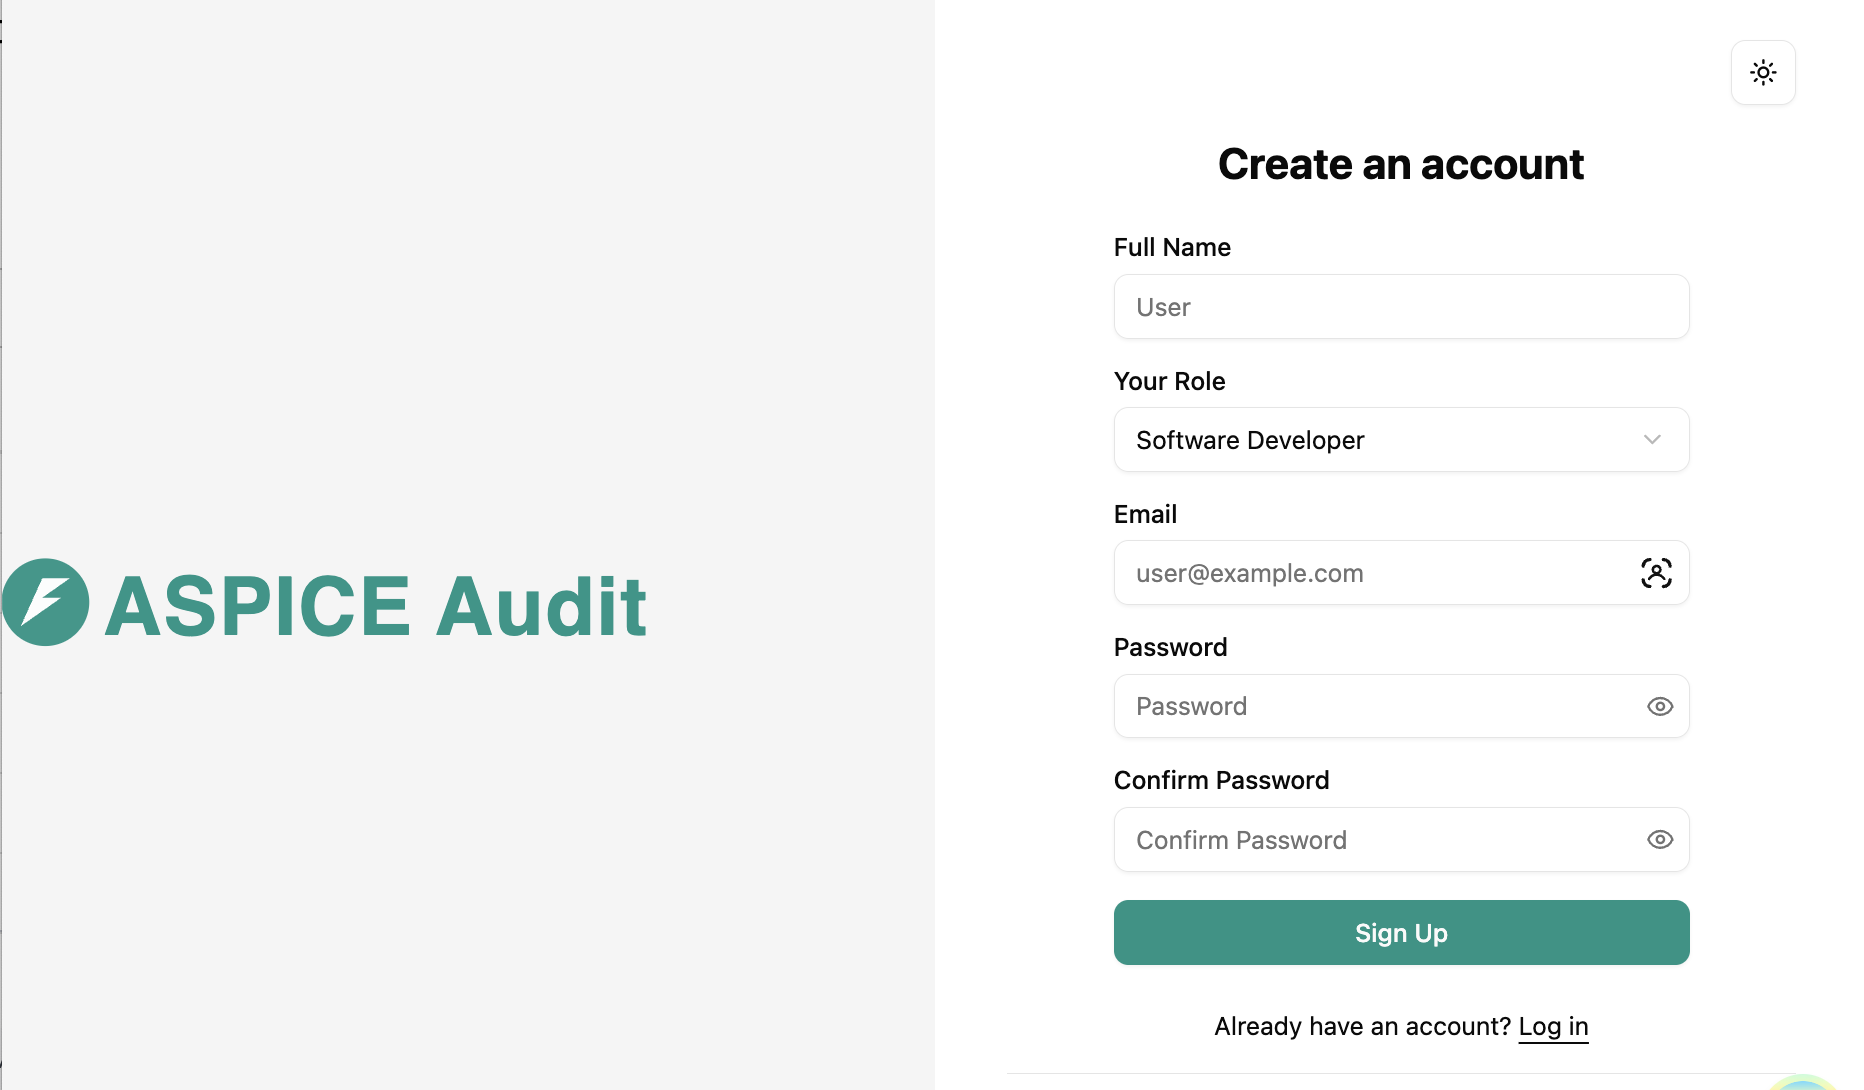
\includegraphics[width=\textwidth]{src/Imp_signup_4.png}
  \caption{Signup page: the \emph{Create an account} form, with the \emph{Your Role} dropdown
  set to a stakeholder role (here, Software Developer).}
  \label{fig:fe-signup}
\end{figure}

\subsection{Assessment Session and Question Interaction}

The audit list (Figure~\ref{fig:fe-audits}) is the stakeholder's home page: it shows any
in-progress session and the history of completed ones, and a single button starts a new
assessment. Starting one creates a session on the backend and navigates to
\texttt{/audit/:sessionId}, which shows exactly one question at a time
(Figure~\ref{fig:fe-session}). Above the question card a progress bar reads ``Question $n$ of
$N$'' and fills to $n/N$, with the denominator taken from the session itself rather than a
fixed constant. Selecting an option enables the \texttt{Next} button, which fires one
\texttt{submitAnswer} mutation. The response is polymorphic: while its status is
\texttt{in\_progress} the next question is written to \texttt{sessionStorage} and rendered in
place; when it comes back \texttt{completed} the app redirects straight to the results route.
Holding the next question in \texttt{sessionStorage} means a mid-session page reload resumes on
the same question instead of restarting the assessment.

\begin{figure}[h]
  \centering
  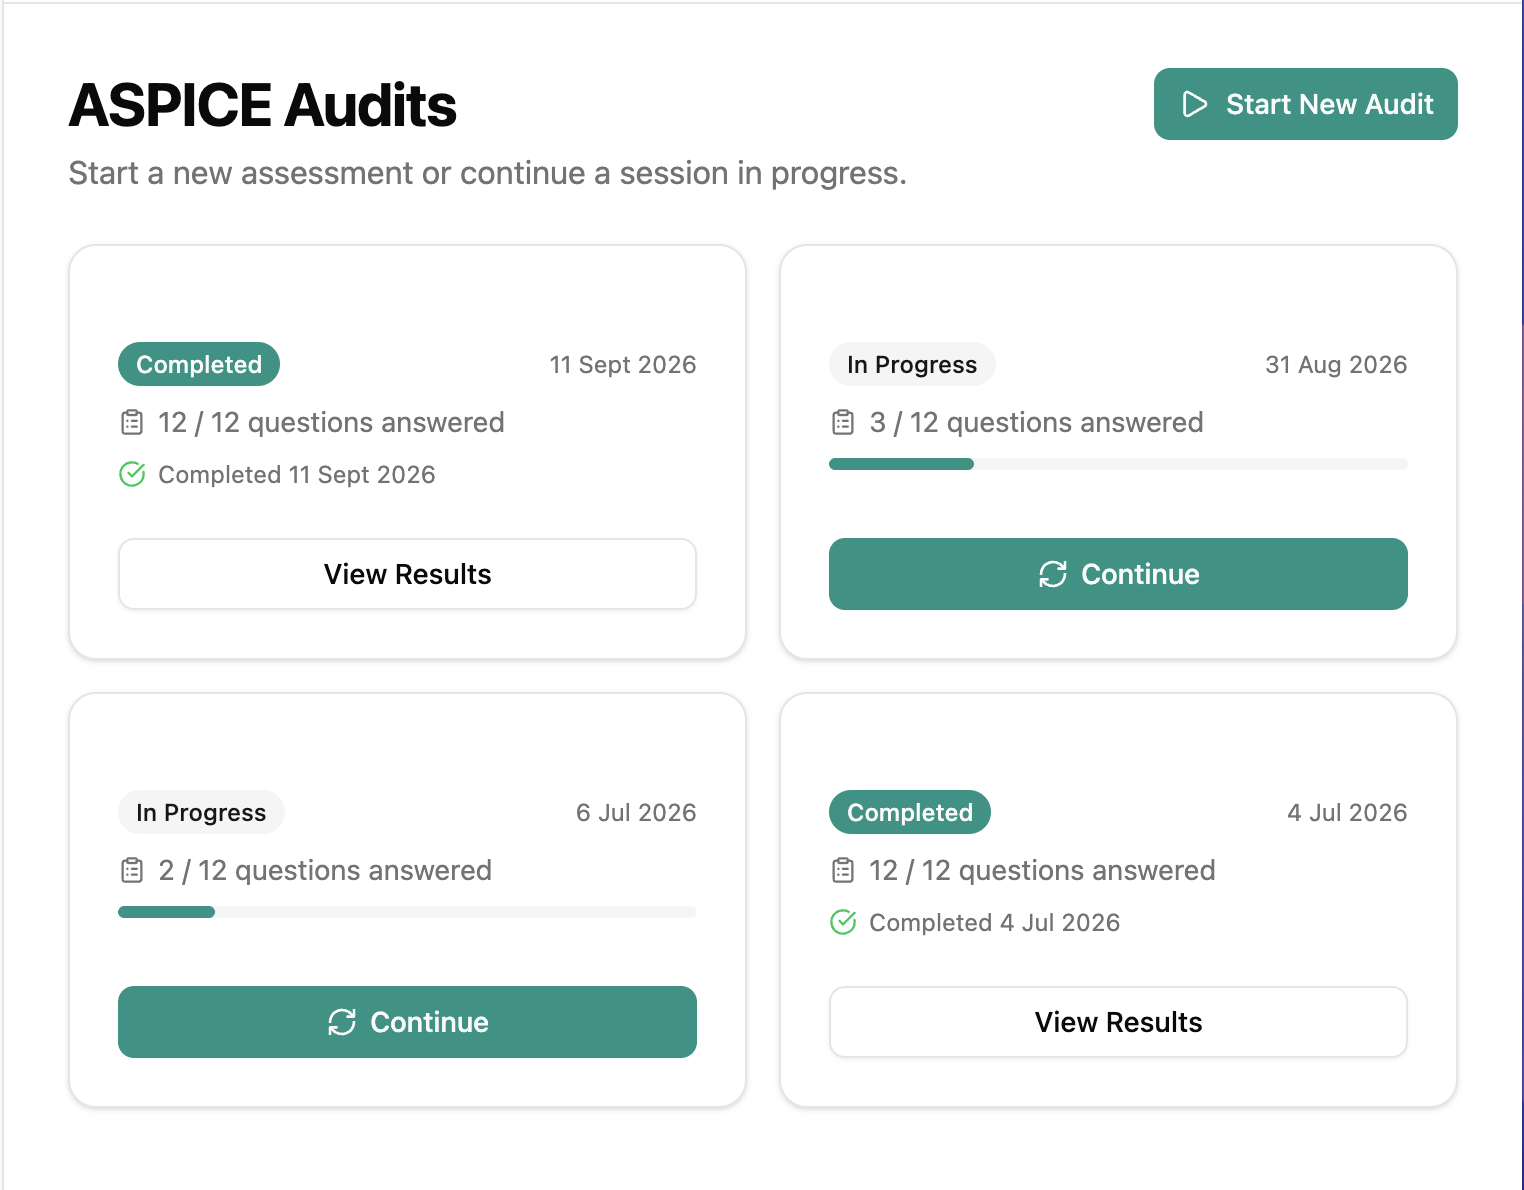
\includegraphics[width=\textwidth]{src/Imp_auditList_5.png}
  \caption{The ASPICE Audits page: in-progress session cards showing questions-answered
  progress, a completed session offering \emph{View Results}, and the \emph{Start New Audit}
  button.}
  \label{fig:fe-audits}
\end{figure}

\begin{figure}[h]
  \centering
  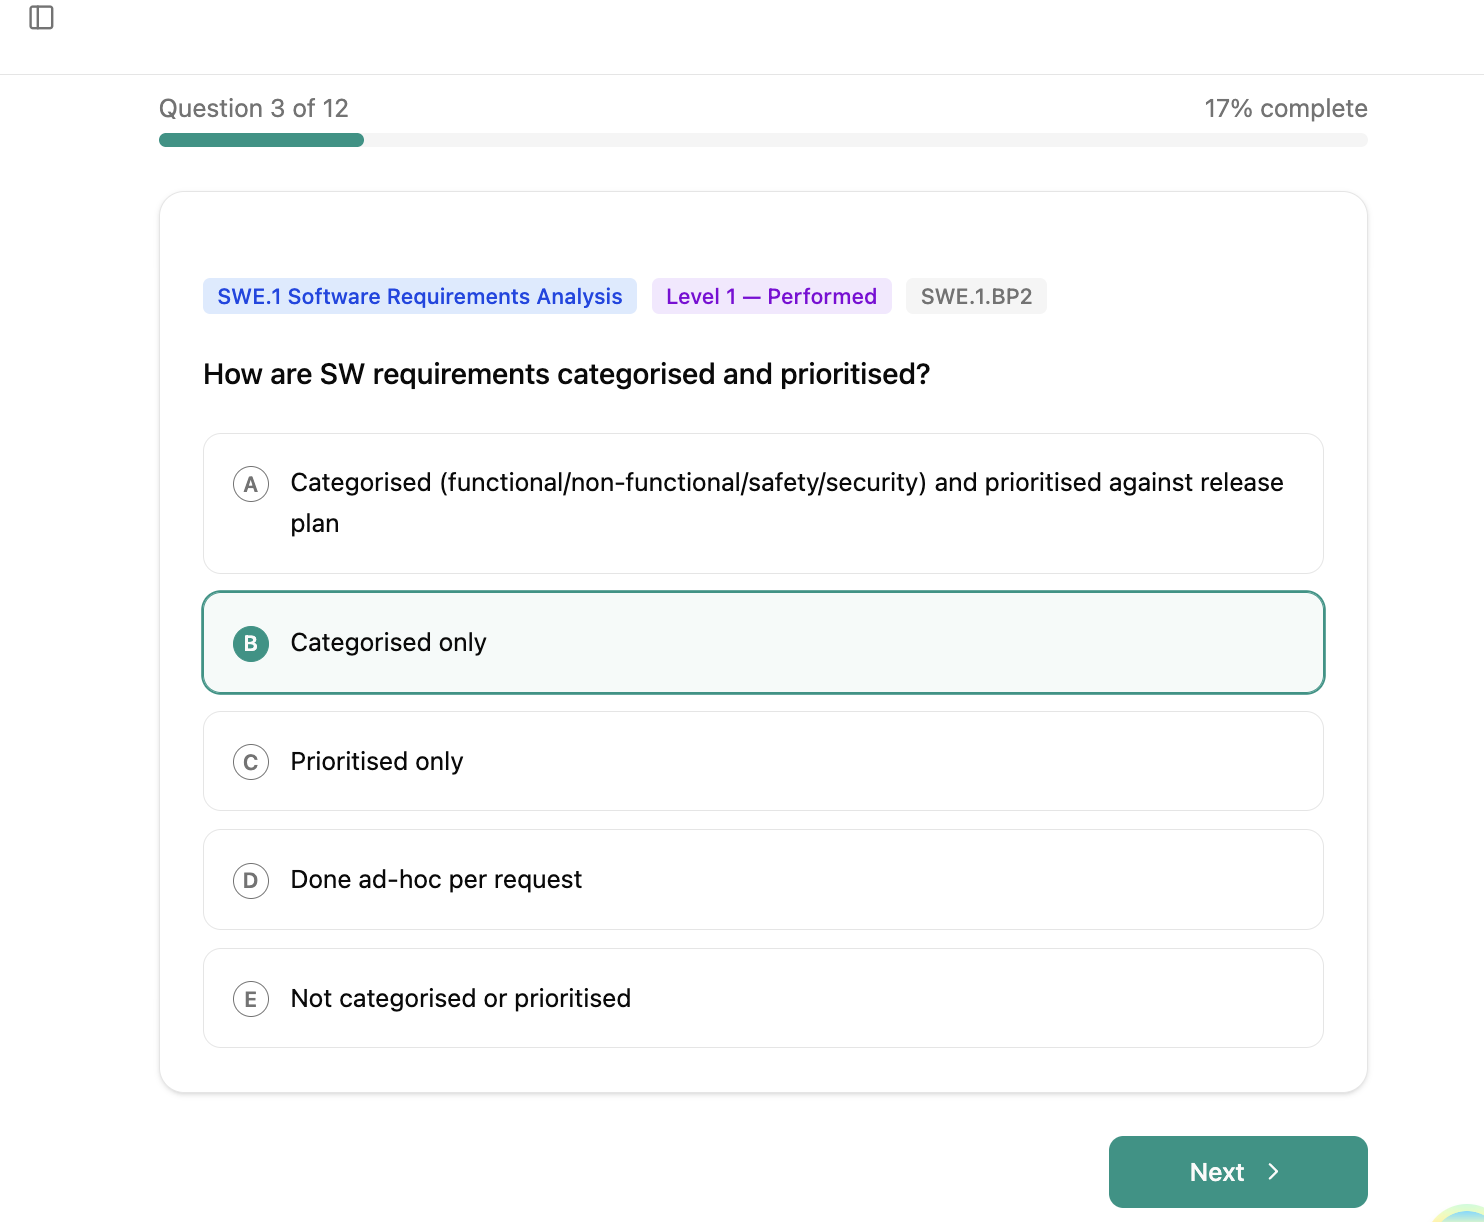
\includegraphics[width=\textwidth]{src/Imp_auditSession_6.png}
  \caption{Audit session page: one question, tagged with its process, level, and base practice.}
  \label{fig:fe-session}
\end{figure}

\subsection{Results Dashboard and Visualization}

The results page (Figure~\ref{fig:fe-results}) reads the stored \texttt{WeaknessResult} through
TanStack Query and renders three views of it. The radar chart is drawn as plain SVG: six
process axes, concentric grid rings, and a filled polygon whose radius on each axis grows with
the weakness score, so a small central shape means a healthy process profile and a large one
means trouble. The process-by-level heatmap is an HTML table whose cells are shaded on the same
four-band scale used throughout the system, with uncovered (process, level) pairs left blank.
Below both, the three highest-scoring pairs are listed together with the recommendation text
carried on each question, turning the scores into concrete next steps. All three views use the
thresholds from Table~\ref{tab:classification-thresholds} and the scores produced by the
classifier in Section~\ref{sec:weakness-classification}.

\begin{figure}[h]
  \centering
  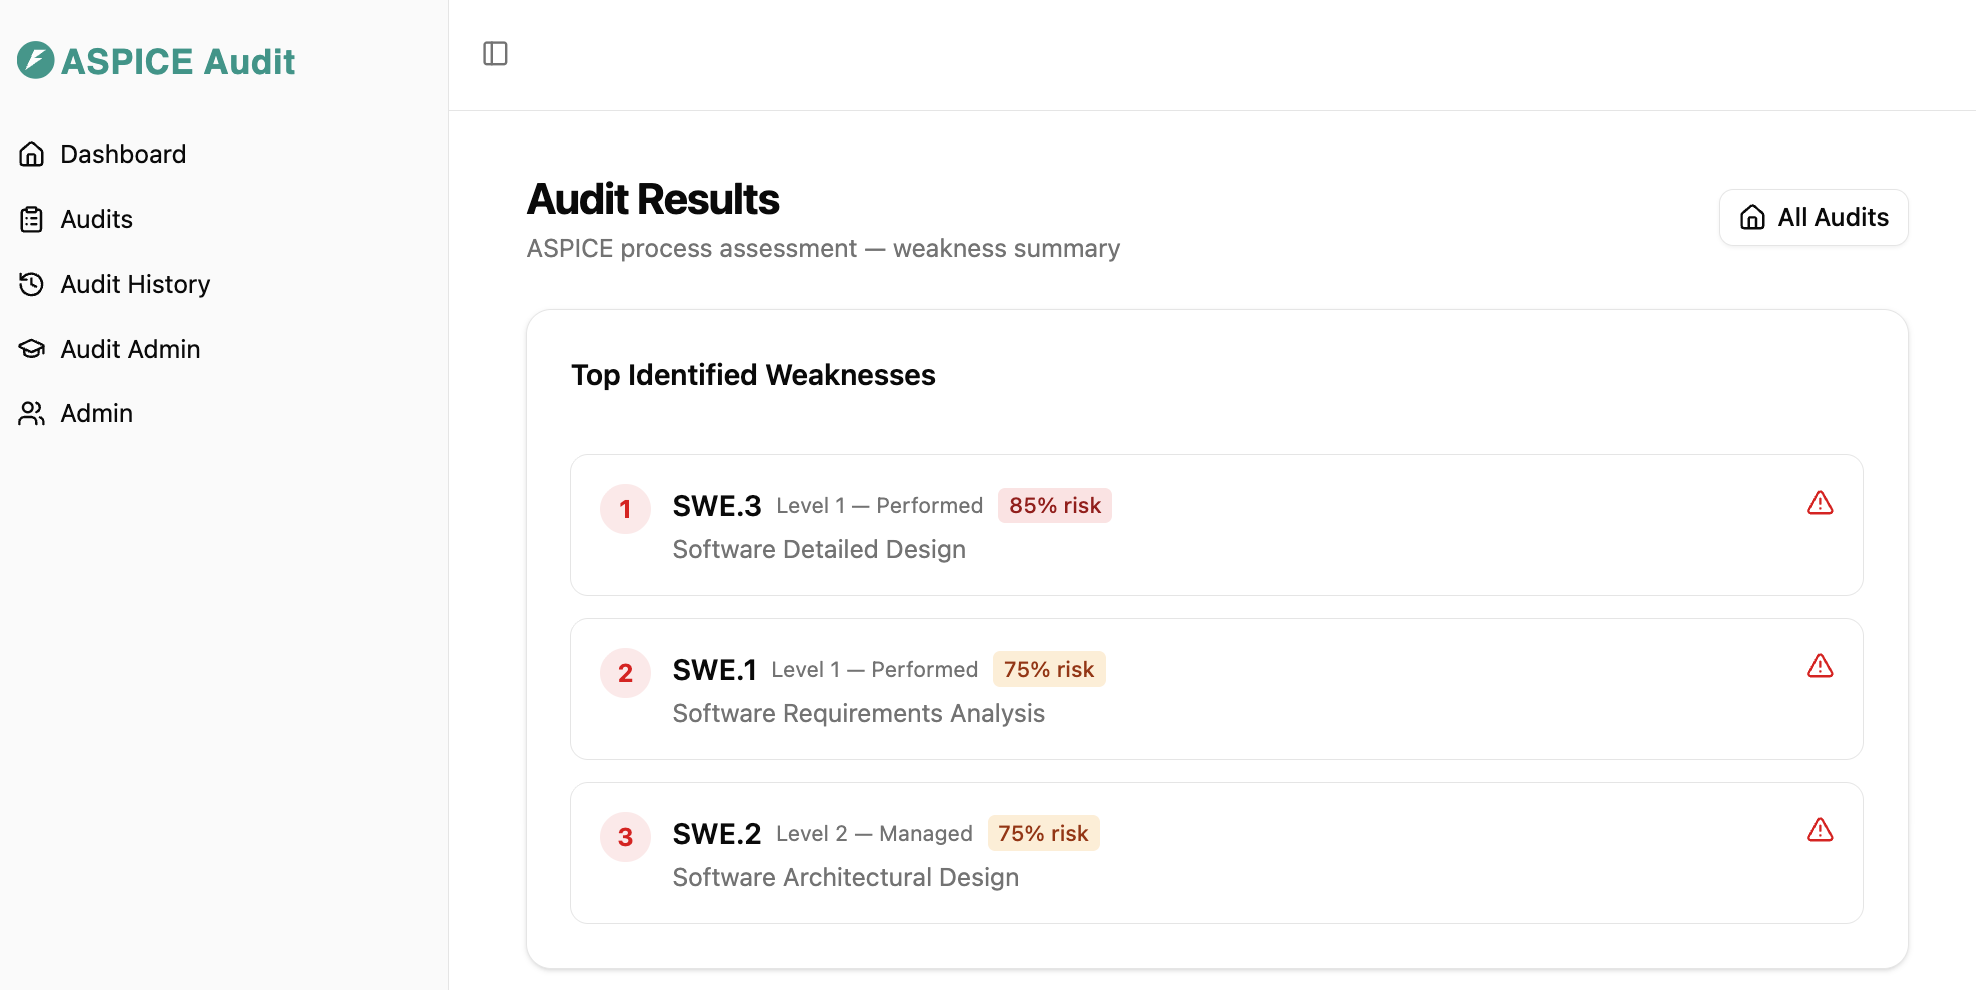
\includegraphics[width=\textwidth]{src/Imp_results_7.png}
  \caption{Results page: \emph{Top Identified Weaknesses}, ranked by risk percentage.}
  \label{fig:fe-results}
\end{figure}

\subsection{Administration and Question Bank Management}

Two pages are visible only to an account with \texttt{is\_superuser} set. The question bank
manager (Figure~\ref{fig:fe-qbank}) lists every \texttt{AuditQuestion} with its options,
filters by process, level, and stakeholder role, and edits a question or its option weights in
a dialog; questions are disabled rather than deleted, so existing sessions keep their
references intact. The analytics dashboard (Figure~\ref{fig:fe-analytics}) aggregates across
sessions: an organisation-wide weakness heatmap, participation counts and completion rates per
stakeholder role, and a table showing how often each question has been selected by the CMAB
engine and its mean reward, the same \texttt{BanditArmState} values from
Section~\ref{sec:cmab-engine}, surfaced for a human reader. Its three feeds come from the
analytics endpoints in Table~\ref{tab:admin-endpoints}.

\begin{figure}[h]
  \centering
  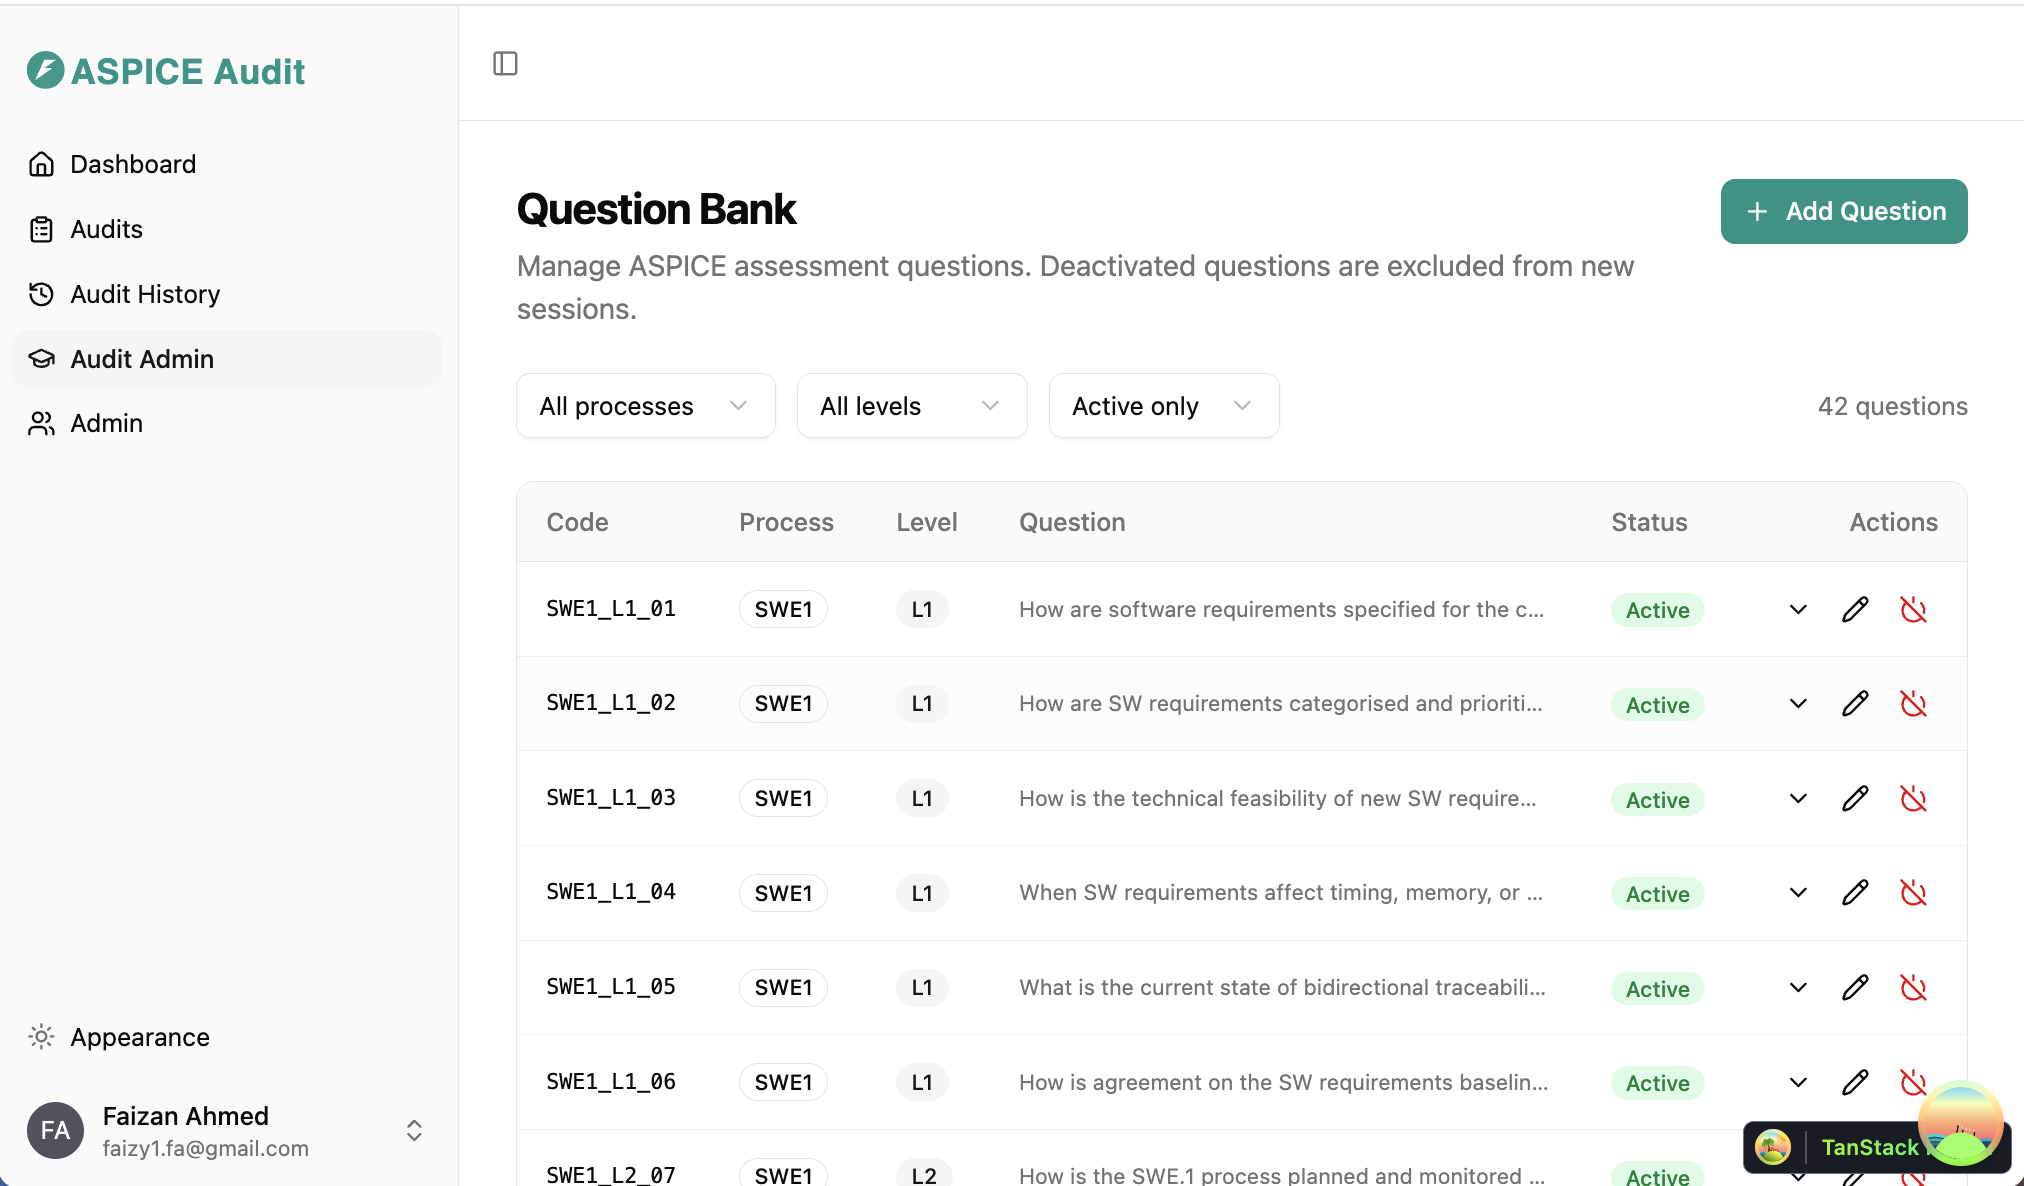
\includegraphics[width=\textwidth]{src/Imp_questionBank_8.png}
  \caption{Question Bank manager: the question table with process, level, and status filters.}
  \label{fig:fe-qbank}
\end{figure}

\begin{figure}[h]
  \centering
  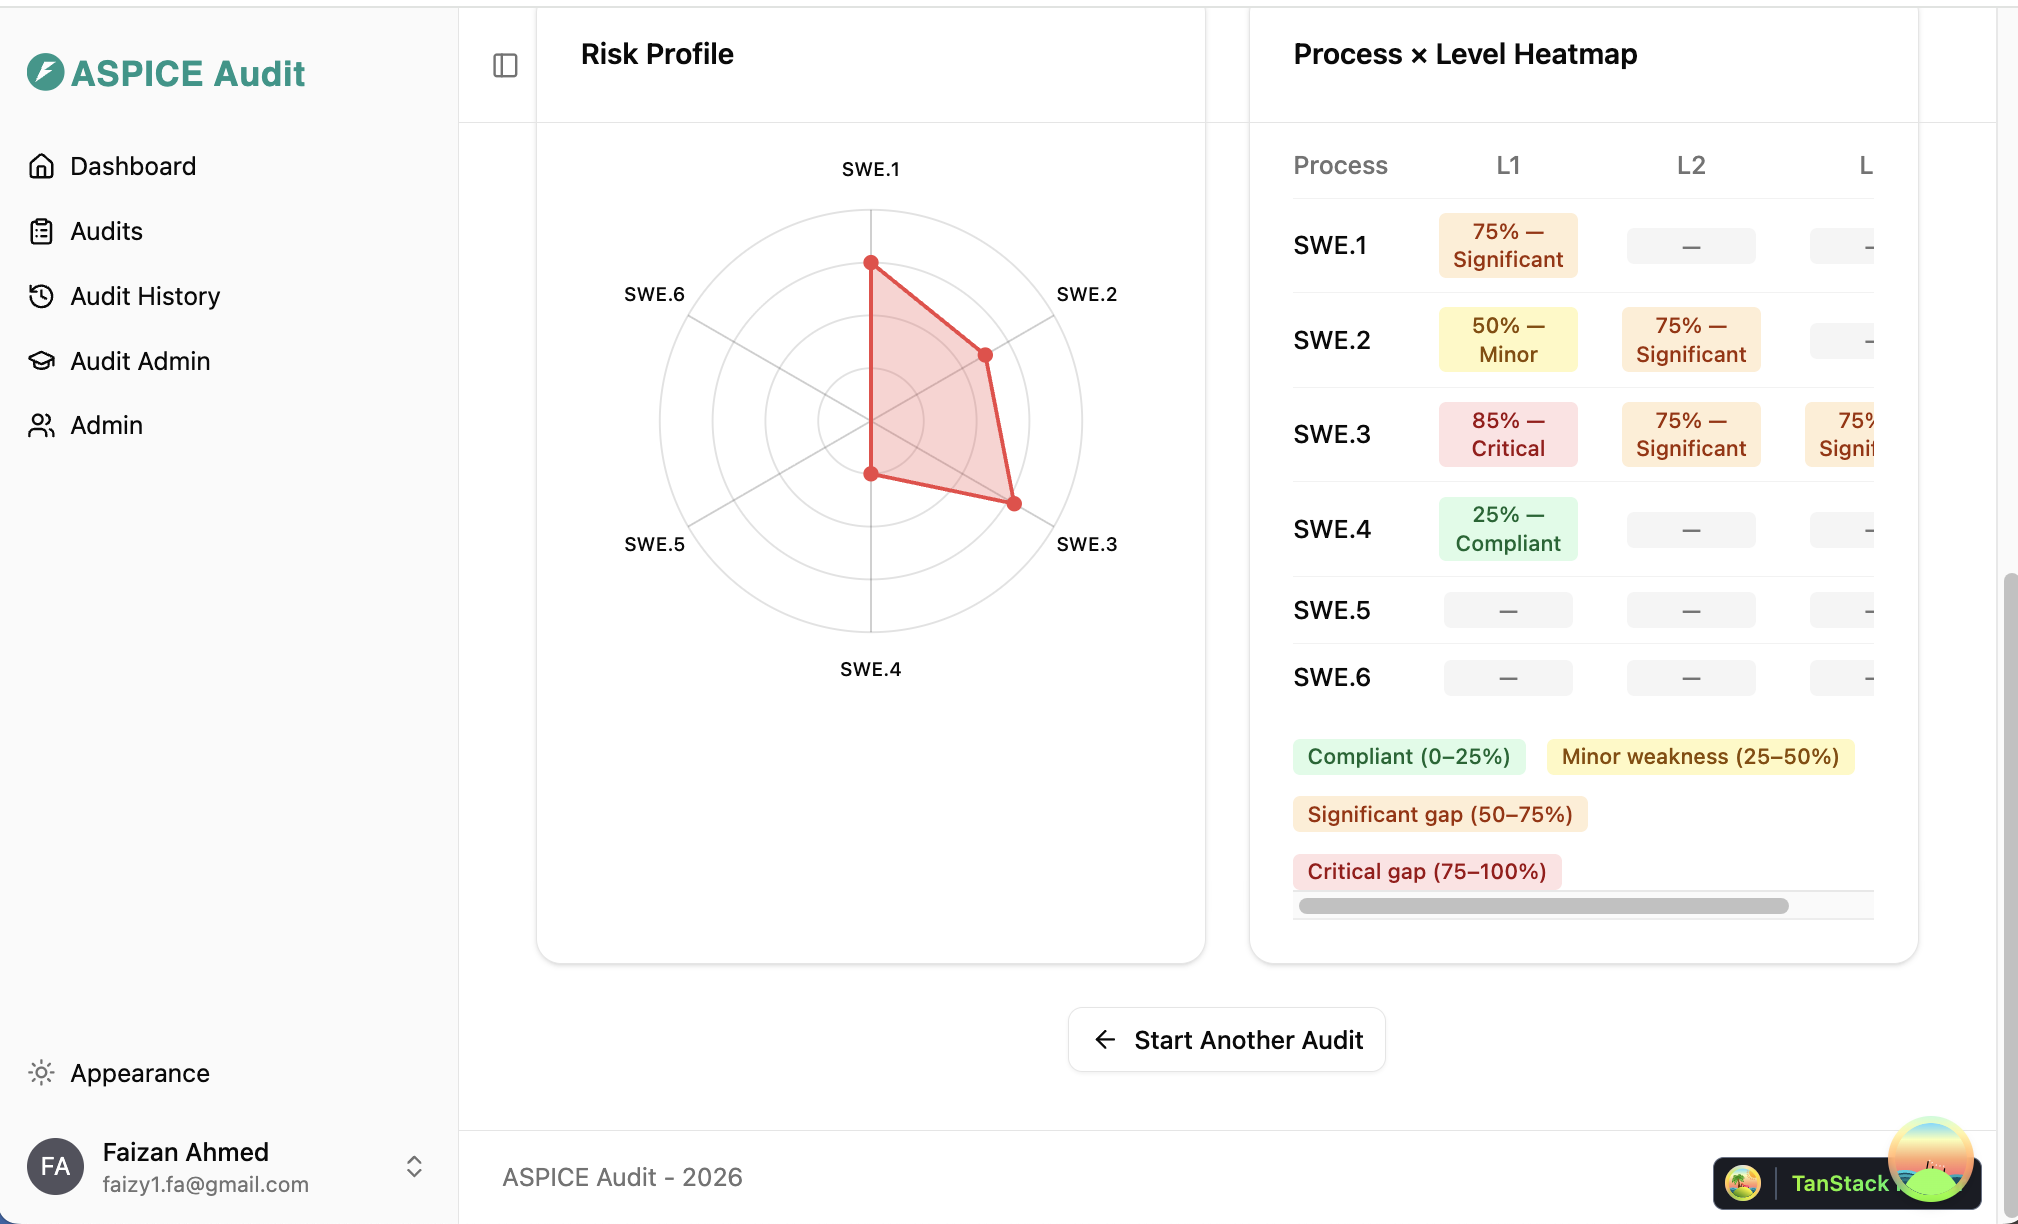
\includegraphics[width=\textwidth]{src/Imp_heatMap_9.png}
  \caption{Results visualisations: the \emph{Risk Profile} radar beside the \emph{Process
  $\times$ Level Heatmap}.}
  \label{fig:fe-analytics}
\end{figure}

\section{Implementation Challenges and Solutions}

\subsection{CMAB State Persistence}

LinUCB keeps, for every question, a $20 \times 20$ matrix $A$ and a $20$-vector $b$. These have
to survive between HTTP requests, since the backend holds nothing in process memory between
calls, and be updated after every answered question, in every session and for every user. They are
stored directly on the question's \texttt{BanditArmState} row as JSON, using SQLModel's JSON
column type, serialized as plain nested lists. On each selection the engine loads the row,
turns the lists back into NumPy arrays, does the linear algebra, and on update writes the arrays
straight back with \texttt{tolist()}. A question that has never been played has no row yet, and
the engine substitutes an identity $A$ and a zero $b$ instead.

\begin{verbatim}
# load:   BanditArmState row  ->  NumPy
A = np.array(arm.A_matrix)          # [[...20...], ...20...]
b = np.array(arm.b_vector)          # [...20...]

# update: rank-1 step, then back to JSON
A += np.outer(context, context)
b += reward * context
arm.A_matrix, arm.b_vector = A.tolist(), b.tolist()
\end{verbatim}

JSON was chosen over the alternatives deliberately. A dedicated vector store would add a whole
component for objects that are a few kilobytes each and only ever fetched by primary key;
\texttt{pickle} would be more compact but opaque and fragile across library versions; JSON is
portable across PostgreSQL and the SQLite used in tests, is readable directly in Adminer, and
diffs cleanly in review. Because $A$ and $b$ are sufficient statistics that already summarise
the entire history of that arm, there is never any need to replay past rounds, and the update
stays constant-time no matter how often a question has been asked.

\subsection{Maintaining Question Selection Constraints}

Before every question, the engine has to recompute which questions are still admissible: a
question is eligible only if it is active, targeted at the current user's stakeholder role, and
not already asked in the current session. This runs on the critical path of every answer, so it
is done as a single filtered query (\texttt{is\_active}, role membership, and \texttt{id} not
in the session's asked list) rather than by loading the bank and filtering in Python. The
result set is small, so the UCB scoring loop that follows only ever runs over a handful of arms.

The awkward case is a session whose eligible pool empties before the question budget is reached,
which can happen for a narrowly-scoped role or simply near the end of a long session. The audit
session service treats ``no eligible questions'' identically to ``budget reached'': it finalises
the session at that point and returns the result, rather than raising an error or serving a
question twice. A session's length is therefore bounded below by the size of the eligible pool
as well as above by the budget, and both limits are enforced in the same branch. Deciding when
the system has genuinely learned enough about a process, rather than simply run out of
questions, is the harder version of this problem, and is what the adaptive session length
described in Chapter~\ref{chap:architecture} is meant to address.

\subsection{Synchronization Between Session State and Database}

Answering one question touches several rows at once: a new \texttt{AuditResponse}, the
question's \texttt{BanditArmState}, the session's \texttt{questions\_asked} list, and, on the
last question, the session's status and a new \texttt{WeaknessResult}. If any of these were
written without the others, the session would be left inconsistent: a recorded answer with no
matching bandit update, or an advanced question pointer with no stored response.
\texttt{submit\_answer} does all of the writes inside a single database transaction and commits
once at the end, so an answer is applied completely or not at all. The processing flow itself is
the one already shown in Chapter~\ref{chap:architecture}
(Figure~\ref{fig:arch-answer-sequence}); the implementation change is only that its steps share
one commit.

Double submission is handled by two guards in the same function. An answer is rejected if its
question ID is not the session's current question, and rejected again if the session is already
completed. A duplicated or late click therefore fails the ordering check instead of recording a
second response or updating an arm twice. The \texttt{questions\_asked} list is stored as JSON
on the session and always rebuilt rather than incremented, so the context vector built in memory
and the list persisted in the database cannot drift apart.

\subsection{Frontend--Backend Integration Issues}

The client and its types are generated from the backend's OpenAPI schema, so a renamed or
retyped field on the backend surfaces as a TypeScript compile error rather than a runtime
\texttt{undefined}. The one endpoint that needed care on both sides is answer submission, which
returns one of two shapes, modelled as a discriminated union on a \texttt{status} literal:
\texttt{in\_progress}, carrying the next question, or \texttt{completed}, carrying the top three
weaknesses. The frontend switches on that single field to decide whether to render
the next question or redirect to the results page, and never has to infer from context that a
session has ended.

Two smaller integration points: the browser calls the API on a different origin during
development (port 5173 against port 8001), so the backend's CORS middleware allow-list is filled
from an environment variable that names the frontend origin per environment; and a single global
error handler on the query client turns any \texttt{401} into a logout and redirect to login,
and every other API error into a toast, so individual pages do not each re-implement error
handling.

\section{Chapter Summary}

This chapter turned the Chapter~\ref{chap:architecture} design into a running system: a FastAPI
and SQLModel backend organised as three services (the CMAB engine, the weakness classifier,
and the audit session service) over a PostgreSQL schema, a 60-question bank seeded
idempotently from the ASPICE base practices, and a React and TanStack frontend built on a
generated, typed API client. Most of the design translated directly: the LinUCB mathematics and
the weakness scoring rules went in essentially as written in Chapter~\ref{chap:architecture}.
The decisions that had to be made at implementation time were narrower: storing the bandit
state as JSON sufficient statistics so no history is ever replayed, drawing a transaction
boundary around a single answer, treating pool exhaustion as a normal end of session, and
keeping the frontend types generated from the backend schema. Whether the system behaves as
intended, and whether contextual selection measurably helps, is the subject of the evaluation in
Chapter~\ref{chap:results}.\footnote{I used AI tool in this Chapter as a verification aid to compare the
described implementation with the functionality actually developed in the web application. The
purpose was to ensure consistency between the concepts presented in this chapter and the
implemented functionality, and to avoid claiming behaviour that was not implemented. See the AI
Referencing section on page~\pageref{app:ai-referencing} for full details.}

\chapter{Results and Evaluation}
\label{chap:results}
% \input{src/results}

This chapter is an evaluation of the system developed in Chapter~\ref{chap:implementation}. It
starts with an explanation of how the evaluation was conducted, then reviews software quality
assurance and functional verification, and finally reviews the pilot sessions themselves -- who
participated, what the CMAB engine actually did when real questions were being answered, and
what the weakness classifier reported. It concludes with a discussion of what the results really
show, and where they are still limited.

\section{Evaluation Approach}

This chapter assesses the system developed in Chapter~\ref{chap:implementation} from three
perspectives: software quality assurance (whether the code itself is correct or not); functional
verification (whether the application performs as expected for a real user); and the pilot
sessions (discussed later in this chapter), to see whether the CMAB engine and weakness
classifier behave as designed when real, non-simulated answers are fed through them. The first
two perspectives can be verified directly on the running system. The third is contingent on the
number of actual sessions completed at the time of writing, and this is not ignored, but rather
discussed later in the chapter under Threats to Validity.

There are two things that are not asserted here. This is not a comparison against a control
group of manual ASPICE assessments, as no such comparison was performed. Where the number of
sessions is small, the results are reported as they were actually experienced: evidence from the
sessions that were actually completed, not evidence that could have been expected from a larger
sample of sessions.

\section{Software Quality Assurance}
\subsection{Unit Testing Strategy and Coverage}

The backend test suite includes 105 test functions across nine files. Of these, three files
directly test the core services this thesis introduces -- \texttt{cmab\_engine.py},
\texttt{weakness\_classifier.py}, and \texttt{audit\_service.py} -- and these three files
account for 56 of the 105 tests.

The three service-level files are pure unit tests: every database call is replaced with
\texttt{unittest.mock.MagicMock}. This is demonstrated by
\texttt{TestBuildContext}, which checks the actual array
\texttt{build\_context} produces for each of the seven stakeholder roles, against known inputs.
This is especially relevant for this thesis, since the CMAB calculations -- the UCB score in
\texttt{TestSelectQuestion}, the $A \leftarrow A + xx^\top$ update in \texttt{TestUpdateArm}, and
the reward formula and its clamping in \texttt{TestComputeReward} -- are each compared against
expected results. The same is true for the classifier's scoring and thresholding in
\texttt{TestComputeScores}, \texttt{TestClassify}, and \texttt{TestGetTopWeaknesses}. These
parts are thus tested individually, and not just indirectly via a full end-to-end request.

\subsection{Unit Test Outcomes}

Table~\ref{tab:test-outcomes} lists every test file in the suite together with its number of
test functions and outcome.

\begin{table}[h]
\centering
\rowcolors{2}{green!5}{white}
\begin{tabular}{l c l}
\toprule
\rowcolor{green!55!black}
\thw{Test file} & \thw{Tests} & \thw{Outcome} \\
\midrule
\texttt{test\_cmab\_engine.py} & 19 & Passing \\
\texttt{test\_weakness\_classifier.py} & 23 & Passing \\
\texttt{test\_audit\_service.py} & 14 & Passing \\
\texttt{test\_users.py} & 27 & Passing \\
\texttt{test\_user.py} & 10 & Passing \\
\texttt{test\_login.py} & 9 & Passing \\
\texttt{test\_backend\_pre\_start.py} & 1 & Passing \\
\texttt{test\_test\_pre\_start.py} & 1 & Passing \\
\texttt{test\_private.py} & 1 & Passing \\
\midrule
\textbf{Total} & \textbf{105} & \\
\bottomrule
\end{tabular}
\caption{Backend test files and outcomes.}
\label{tab:test-outcomes}
\end{table}

All 105 tests pass.

\subsection{Static Analysis / Linting Outcomes}

The backend was tested with two kinds of automated checks. The first identifies style issues and
common mistakes in the code, such as an unused import or code that might cause trouble later on.
The second is a type checker, run in its strictest available setting through every function in
the backend, which verifies that the values being passed around are what each piece of code
expects to receive.

The style checker found seventeen small issues in total, most of which can be corrected
automatically without any manual editing. Almost all of these sit in the test code, not in the
code that actually runs in production.

The type checker reported forty-one warnings, but the vast majority of these are not a major
concern, and are typical of this kind of project. The first category relates to how the database
library represents queries internally: even though a dynamically generated query is correct and
always returns the right result, the type checker cannot always confirm that it takes the form
it expects. This is a known limitation of combining a strict type checker with this particular
database library, not proof of faulty logic. The second category is much smaller, and concerns a
few places where a value that is allowed to be empty is treated as though it definitely is not.
In each case, the surrounding code actually guarantees the value is present by the time it is
accessed, which is why the code is correct, but the type checker has no way to see that same
guarantee just from reading the function in isolation. These remaining cases are still worth
tightening, since a reader, or a future change to the code, cannot assume that guarantee always
holds and should check it directly.
\section{Functional Verification}
\label{sec:functional-verification}
\subsection{Test Case Design and Health Checks}

\begin{figure}[h]
  \centering
  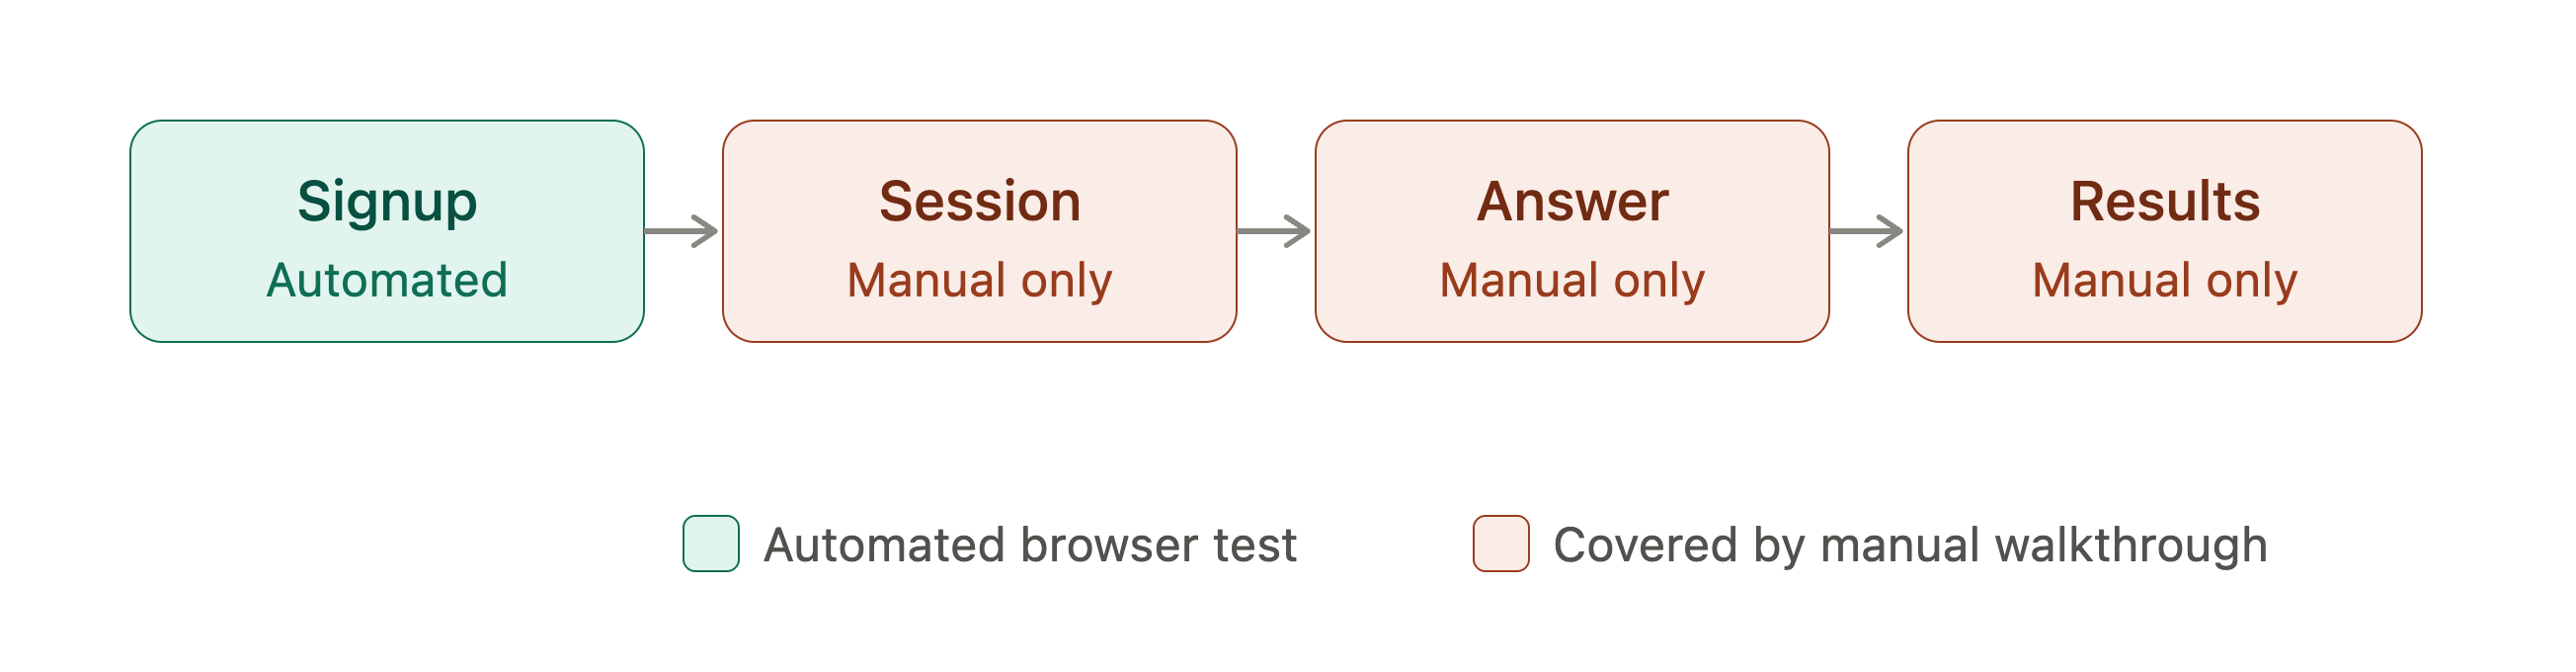
\includegraphics[width=\textwidth]{src/Results_1.png}
  \caption{Test coverage across the four step flow: only Signup has automated browser tests.}
  \label{fig:test-coverage-flow}
\end{figure}

Figure~\ref{fig:test-coverage-flow} summarises how these four steps are actually verified. Only
one of the four has automated browser-based tests behind it: account creation. These tests
verify valid credentials, invalid email, weak or mismatched passwords, missing fields, and the
proper rejection of incomplete submissions. A similar, but distinct, part of the system, logging
back in, is protected the same way, including redirecting a user away from protected pages when
they are not logged in or hold an invalid session token. Neither of these tests, however, covers
the role selection field added at account creation, as described in
Chapter~\ref{chap:architecture}, and there is currently no automated test for starting a
session, answering a question, or viewing results -- the actual ASPICE-specific steps this
thesis is built around. This gap is closed here with a walkthrough of the deployed system rather
than a scripted test, but it is worth making explicit rather than leaving implicit.

At the infrastructure level, health is monitored continuously rather than once. The backend has
a small status endpoint that simply returns whether it can respond, and the surrounding
container setup calls that endpoint automatically every few seconds. As of this writing, every
part of the running system, the backend, the database, the frontend, and the administration
tool used during development, is reported as healthy and running.

\subsection{End-to-End Flow Walkthrough}

Figures~\ref{fig:e2e-signup} through~\ref{fig:e2e-heatmap} illustrate one actual session run on
the deployed system, from account creation to the final results. This is not a record of every
field or click; it is meant to demonstrate that the application actually works as described in
Chapter~\ref{chap:architecture}, and that this was tested on the running application rather than
assumed from the code.

\begin{figure}[h]
  \centering
  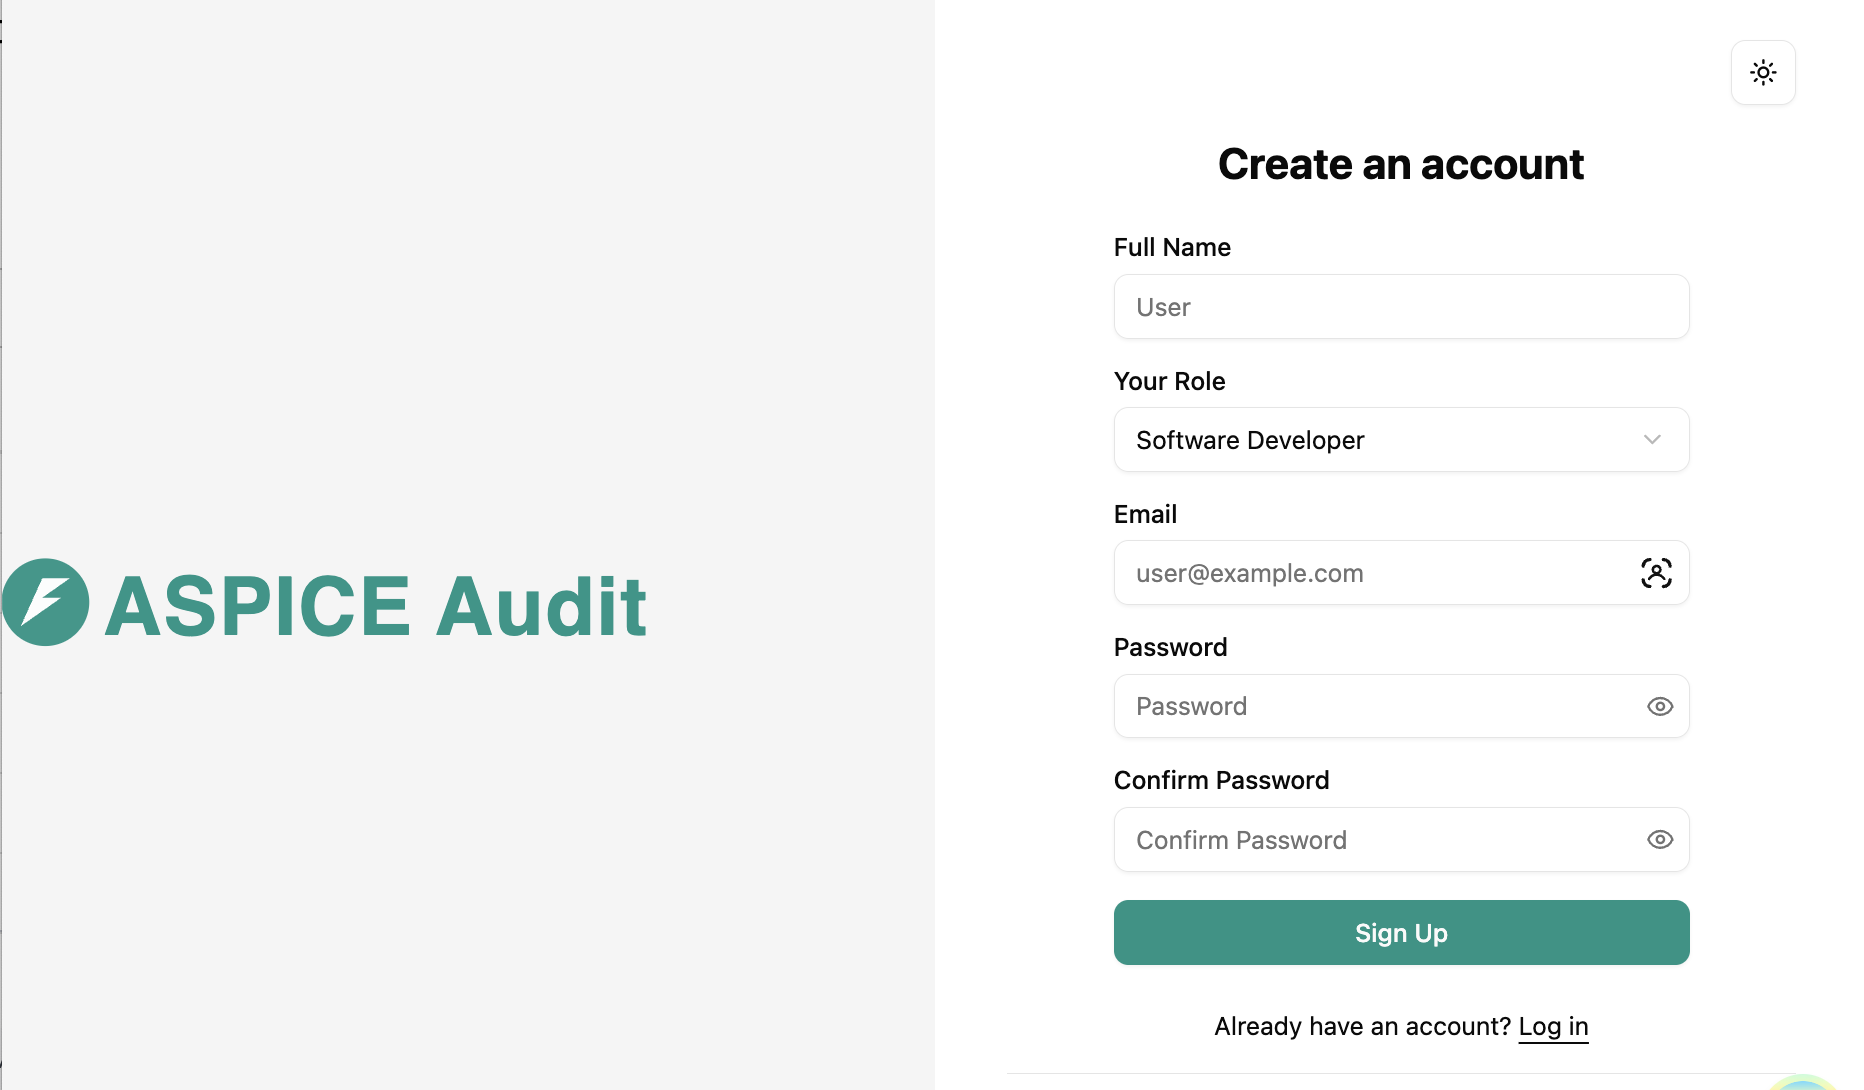
\includegraphics[width=\textwidth]{src/Imp_signup_4.png}
  \caption{Signup, with a stakeholder role selected from the seven defined in
  Chapter~\ref{chap:architecture}.}
  \label{fig:e2e-signup}
\end{figure}

When a stakeholder signs up, a new account is created with a stakeholder role assigned at signup
(Figure~\ref{fig:e2e-signup}), confirming that the signup flow, including the role assignment,
works end to end.

\begin{figure}[h]
  \centering
  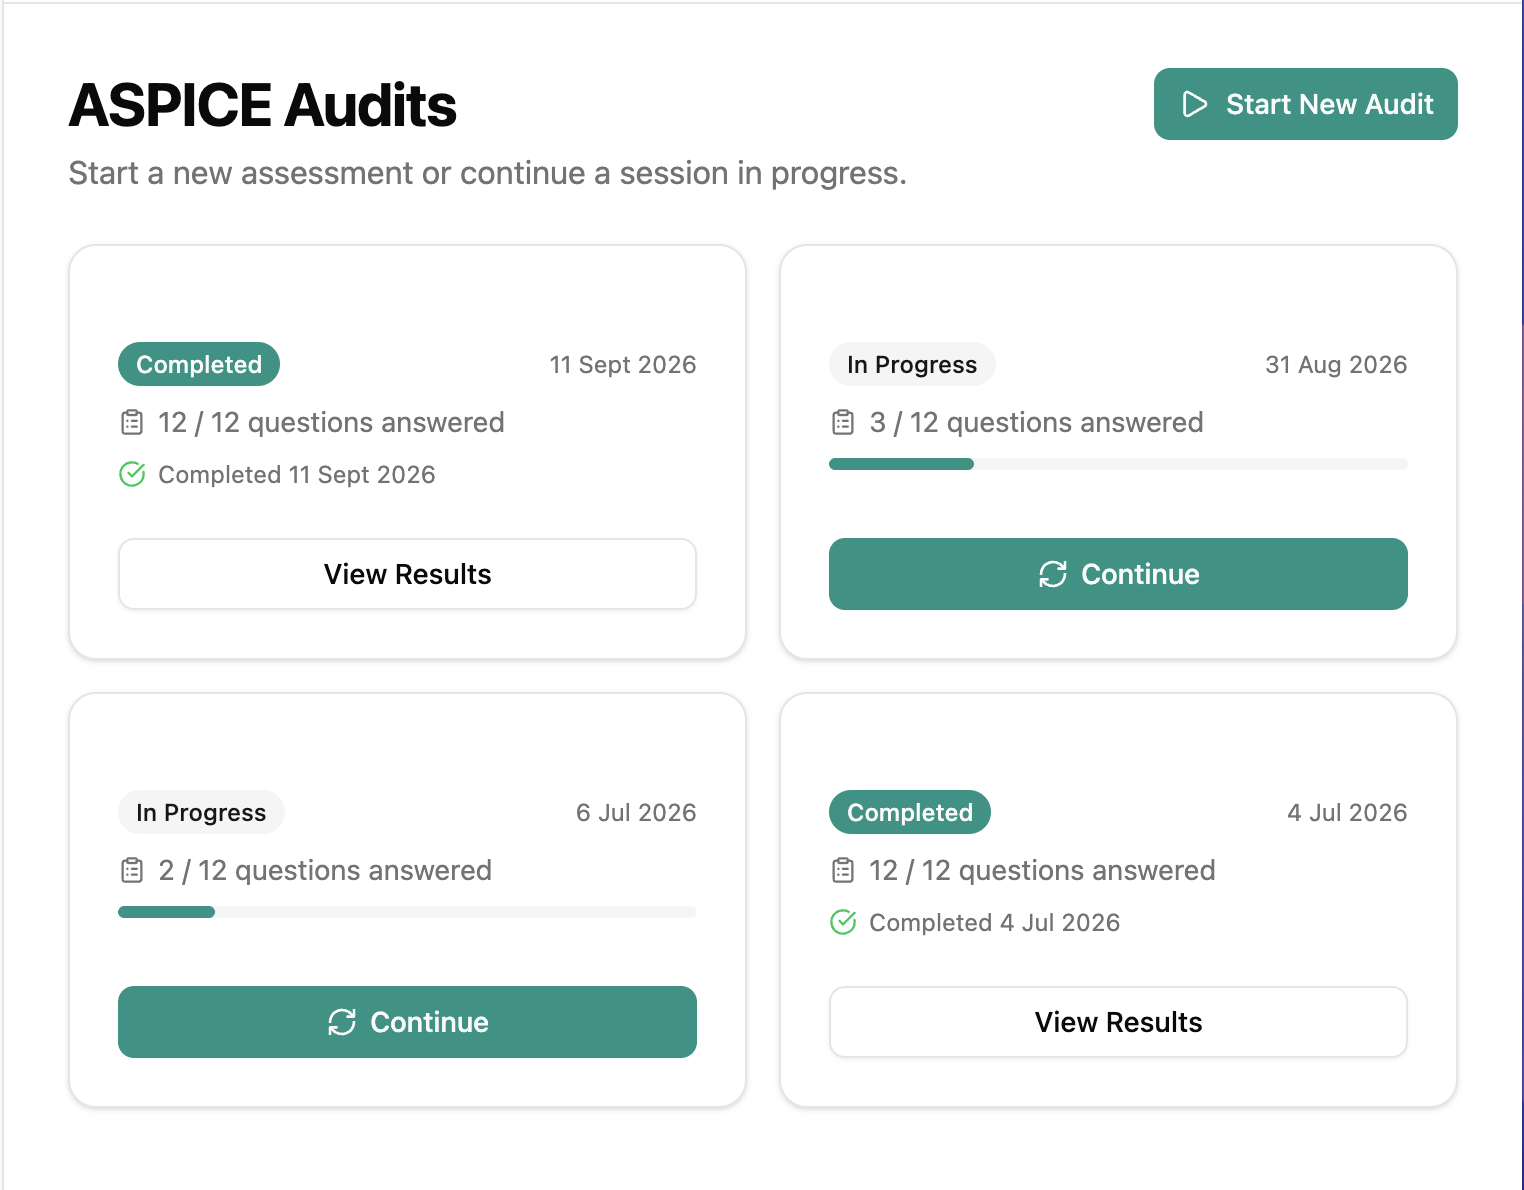
\includegraphics[width=\textwidth]{src/Imp_auditList_5.png}
  \caption{The audits list for one real account, showing sessions in progress and completed.}
  \label{fig:e2e-audits}
\end{figure}

The audits list (Figure~\ref{fig:e2e-audits}) confirms that sessions are stored properly and can
be retrieved later: it shows several real sessions against this account, some still in progress
and one completed, rather than a single session that only ever existed briefly.

\begin{figure}[h]
  \centering
  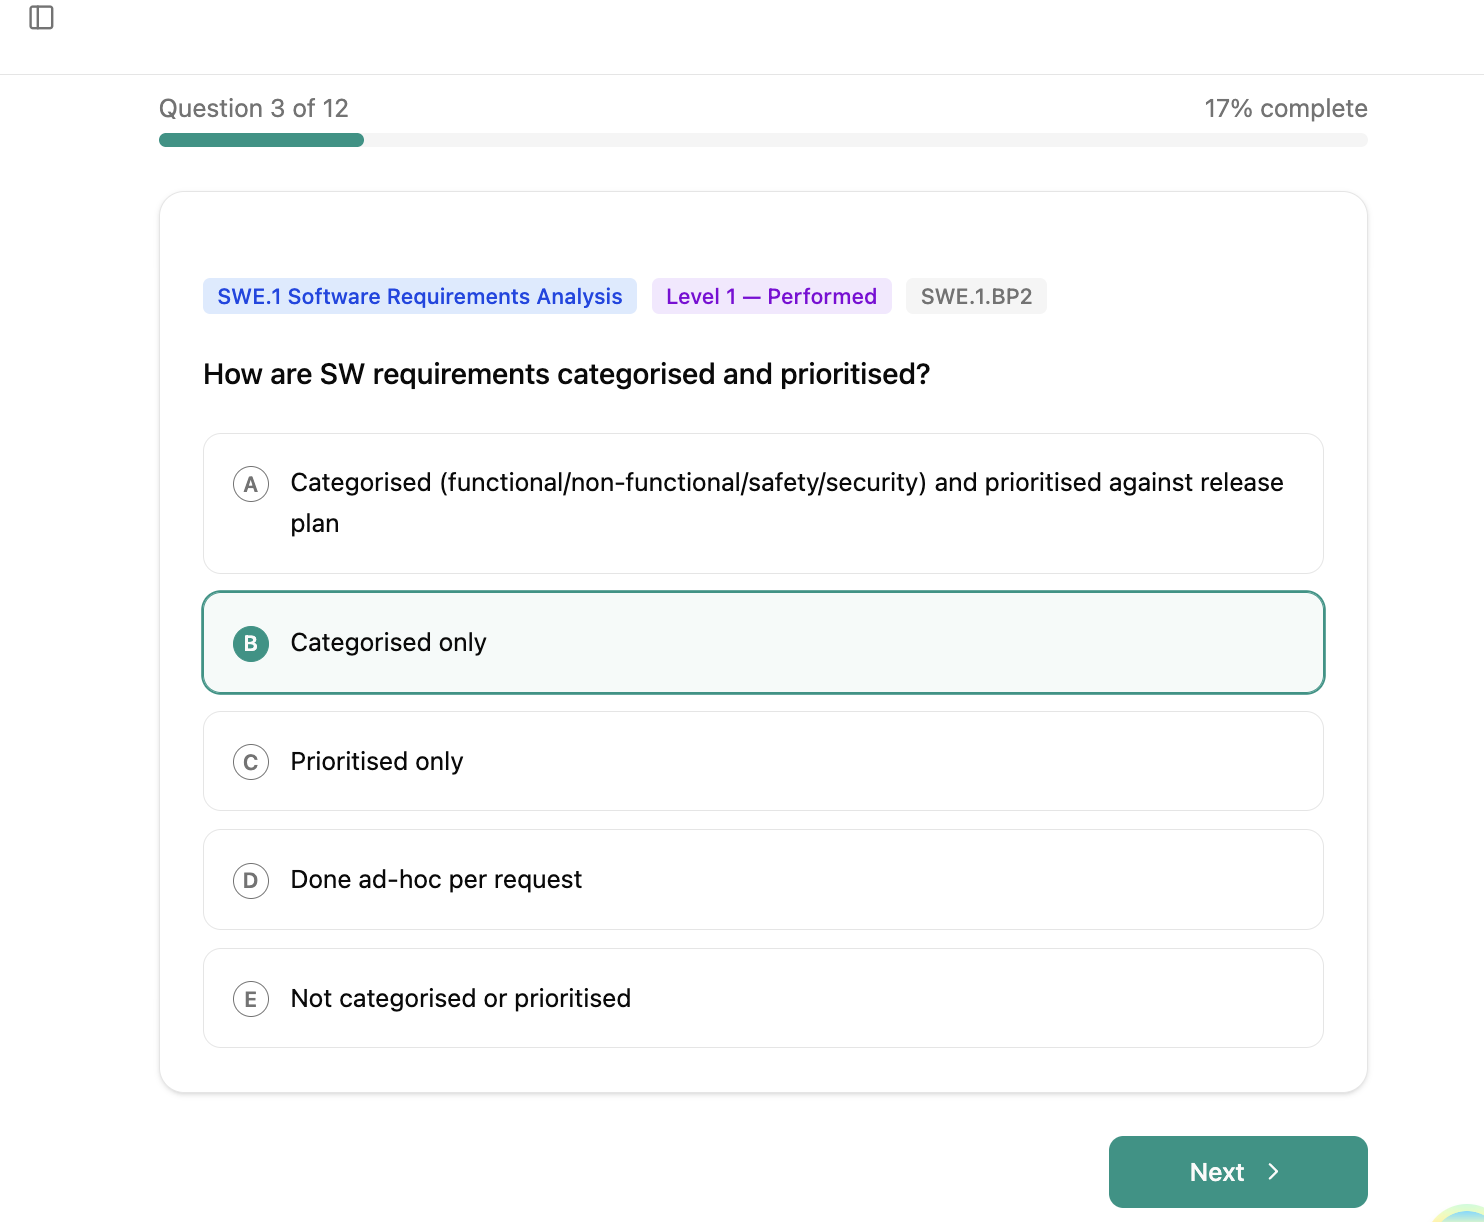
\includegraphics[width=\textwidth]{src/Imp_auditSession_6.png}
  \caption{One question from partway through the completed session.}
  \label{fig:e2e-session}
\end{figure}

One question from partway through that session is shown in Figure~\ref{fig:e2e-session}, with
its five answer options displayed exactly as they are stored in the question bank, confirming
that questions are served and presented correctly, one at a time.

\begin{figure}[h]
  \centering
  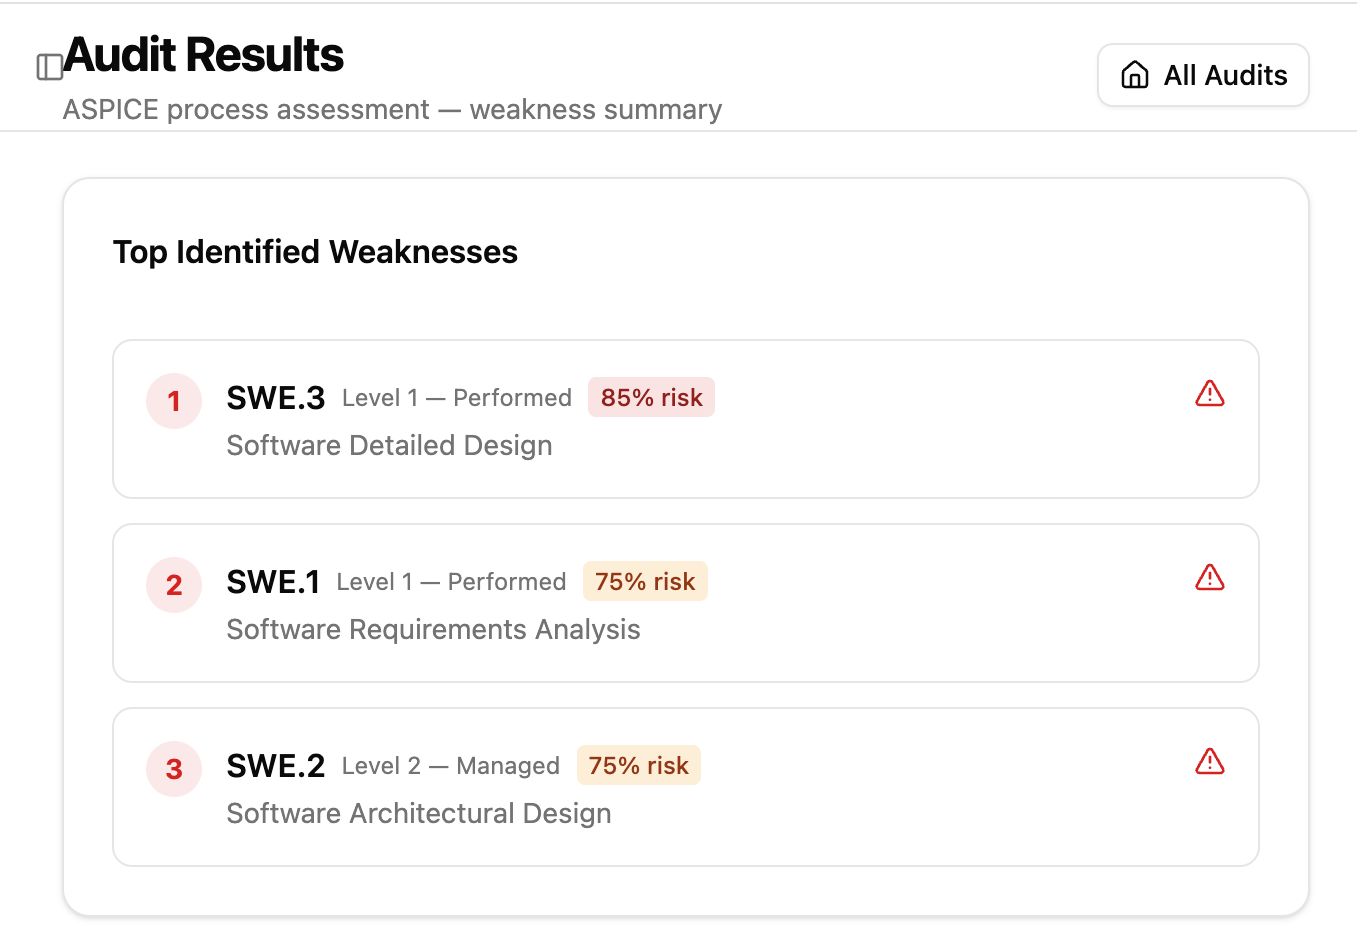
\includegraphics[width=0.8\textwidth]{src/Results_per_session_2.png}
  \caption{The top weaknesses identified for the completed session.}
  \label{fig:e2e-results}
\end{figure}

\begin{figure}[h]
  \centering
  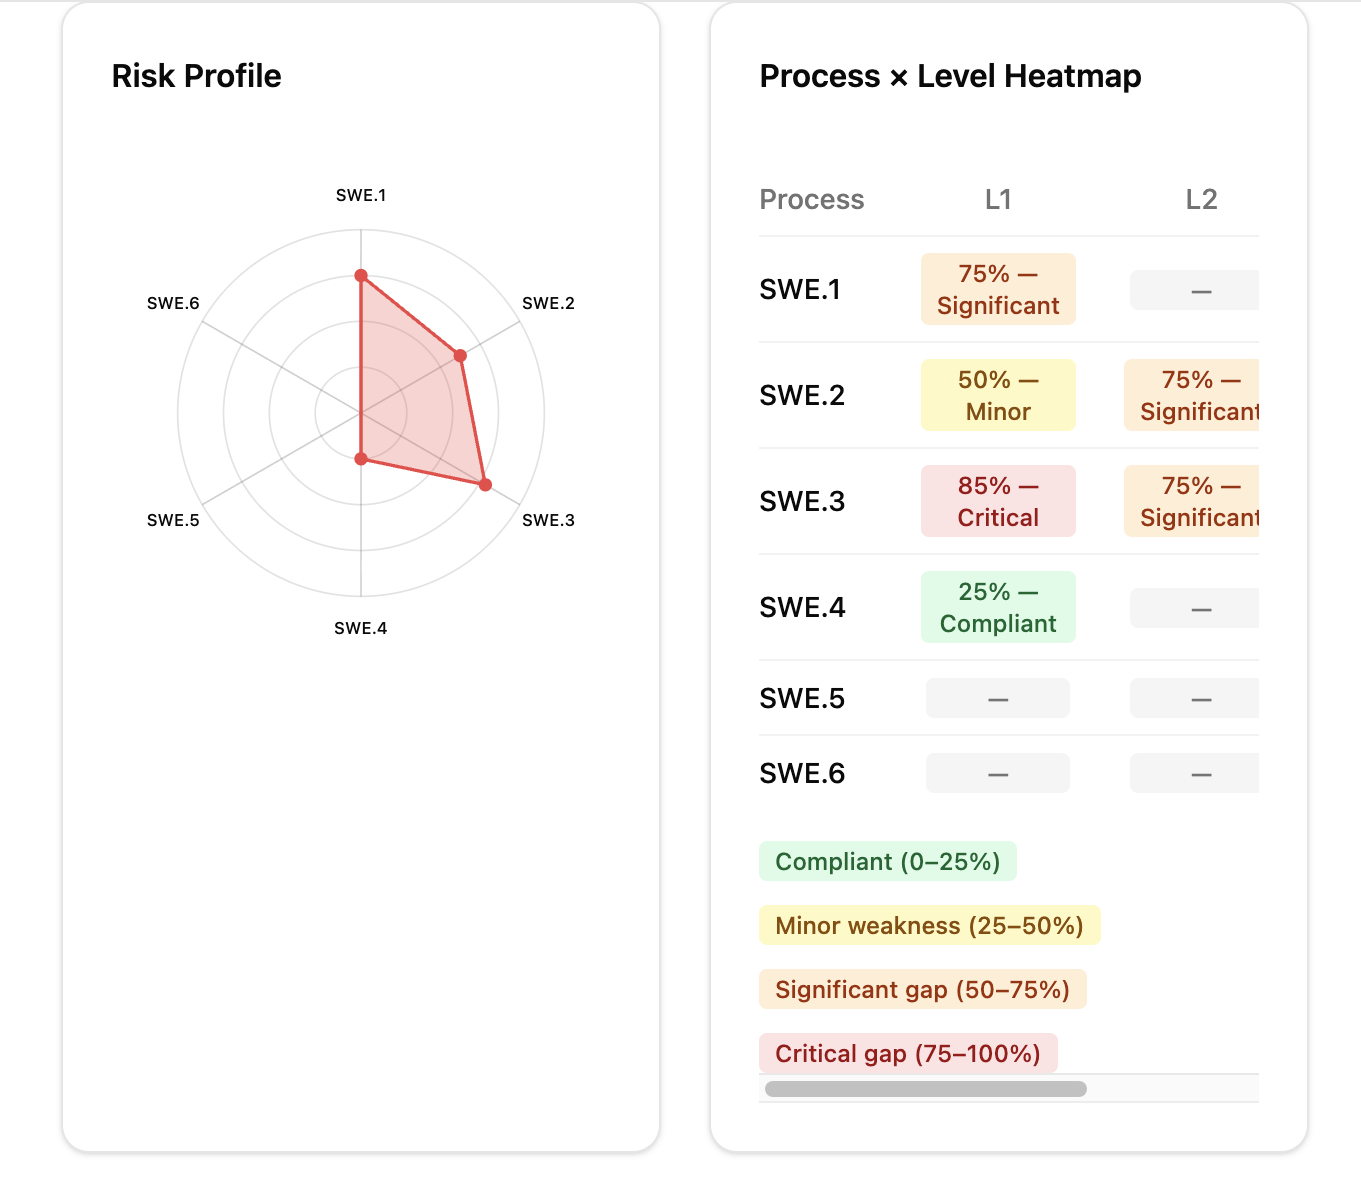
\includegraphics[width=0.8\textwidth]{src/Results_per_session_1.png}
  \caption{The same session's radar chart and process-by-level heatmap.}
  \label{fig:e2e-heatmap}
\end{figure}

Once every question in the session had been answered, the weakness classifier automatically
produced a result, shown in Figures~\ref{fig:e2e-results} and~\ref{fig:e2e-heatmap}: a ranked
list of the most significant weaknesses, a radar chart, and a full heatmap across every process
and level. This confirms that the scoring rule described in Chapter~\ref{chap:architecture}
works as intended on a real submitted session, not only on a worked example.

\begin{figure}[h]
  \centering
  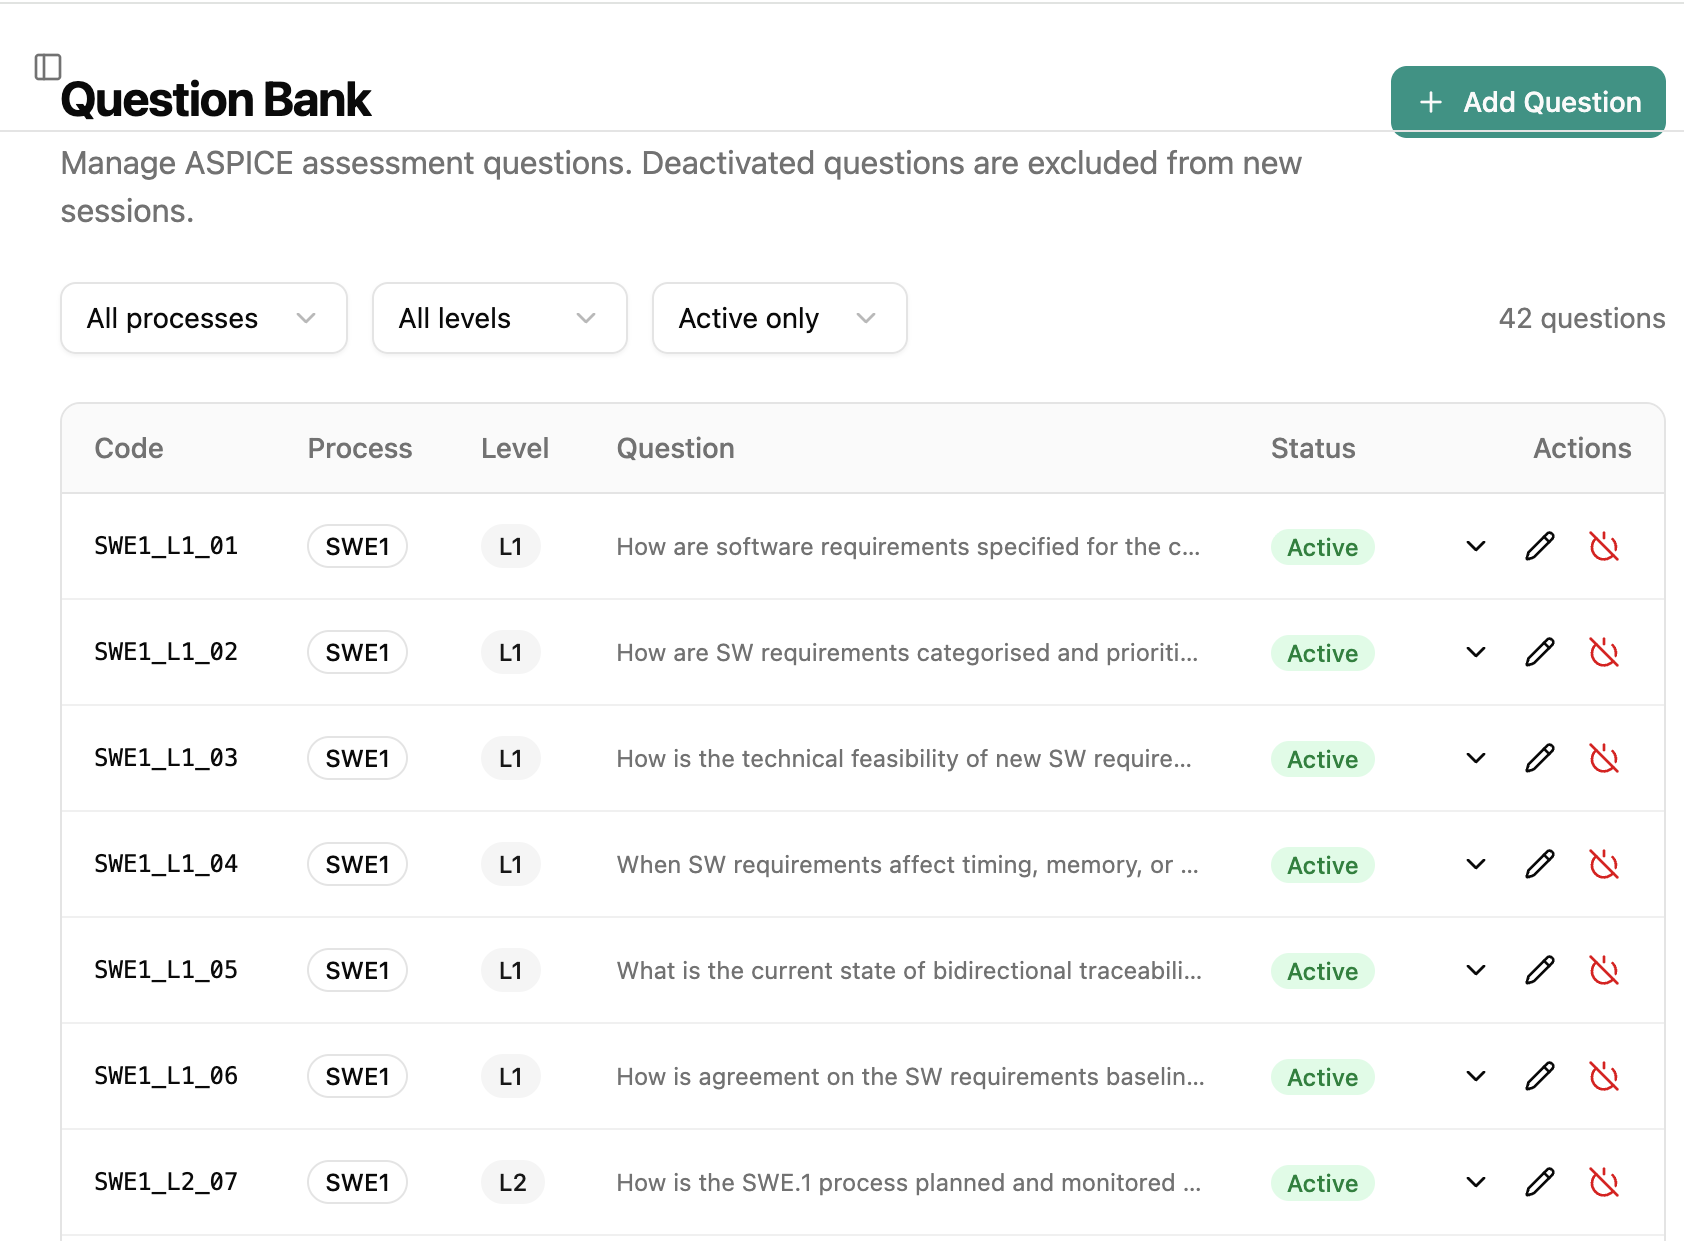
\includegraphics[width=\textwidth]{src/Results_questions.png}
  \caption{The question bank manager, listing all 60 active seeded questions.}
  \label{fig:e2e-questionbank}
\end{figure}

For completeness, Figure~\ref{fig:e2e-questionbank} shows the administrator view of the same
system, listing all 60 active questions seeded for SWE.1--SWE.6, filterable by process, level,
and active status.

\subsection{Smoke Test Outcomes}

Smoke testing of this system is performed manually, as it would be for a real user or
administrator, using the same basic flows, and ensuring that the various components of the
application continue to work together from beginning to end.

In this way three things are checked. The user account itself is secure: the user has to sign
up and log in properly to access anything else, and cannot see or continue another user's
session. Second, a full session can be completed from start to finish: a user can answer every
question in a session in turn until the session ends. Third, at the end of the session, an
administrator can see exactly where the problem lies, including which process and level came
out weakest, and which question and answer pointed to that weakness.

The walkthrough in the previous subsection is a complete run of this manual smoke test, and it
passed: an account was created with a role, a full session was completed by answering every
question in sequence, and the resulting weaknesses were visible afterward, both to the account
that completed the session and, from the administration side, in the aggregate view across
sessions.
\section{Pilot Usage Sessions}

The functional verification walkthrough in Section~\ref{sec:functional-verification} already
demonstrated the system functioning end to end on one account. This section is about a larger
pilot, which involved real sessions across all the stakeholder roles the system identifies,
rather than just one.

\subsection{Participants and Stakeholder Roles Represented}
\label{sec:pilot-participants}

The pilot was conducted by the author in seven different stakeholder roles, as defined in
Chapter~\ref{chap:architecture}: Software Developer, Software Architect, Project Manager,
ASPICE Assessor, QA Engineer, Test Engineer, and Team Lead. This is not an independent external
participant pilot, but one of self-administration, and this is clearly stated in
Chapter~\ref{chap:conclusion}. Answers were not given against one fixed, consistent real
project; the author answered each question from general domain knowledge of how a stakeholder in
that role would typically respond, rather than by consulting one specific system's actual
requirements, architecture, or test records. Consequently, this pilot is a feasibility test of
the mechanism -- whether question selection, weakness scoring, and the results dashboard behave
sensibly end to end on real, human-entered answers -- and not a validity study of any single
project's actual ASPICE compliance; the latter would require independent stakeholders answering
against one shared, real codebase, and is left to future work
(Section~\ref{sec:threats-to-validity} returns to this distinction). What it does offer, that the
single-account walkthrough in Section~\ref{sec:functional-verification} could not, is real usage
data broken out by role, which is exactly what the CMAB engine's context vector is geared to
respond to.

\begin{figure}[h]
  \centering
  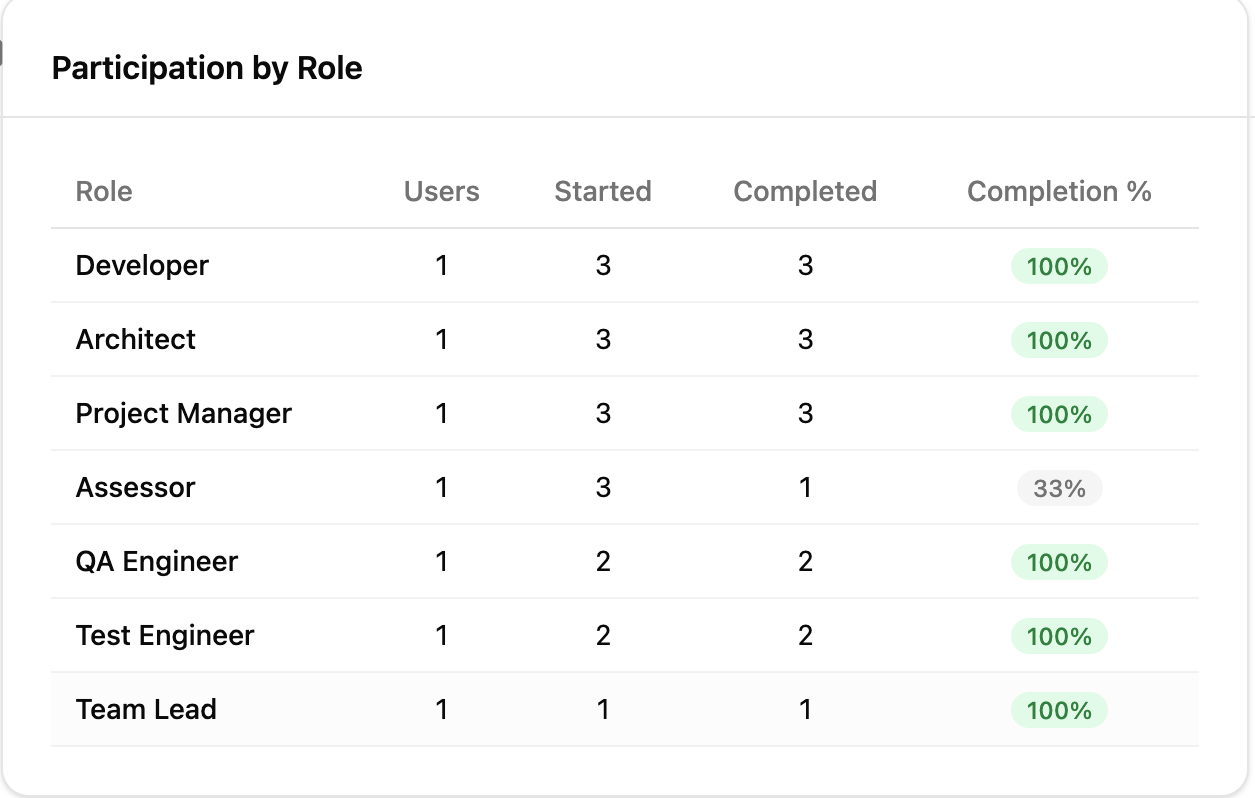
\includegraphics[width=\textwidth]{src/Results_admin_dashboard_participation.png}
  \caption{Participation by stakeholder role, read from the system's own analytics.}
  \label{fig:pilot-participation}
\end{figure}

Figure~\ref{fig:pilot-participation} shows participation broken down by role: six of the seven
roles completed every session they started. The ASPICE Assessor account is the exception: three
sessions were started under this role and only one was completed, a 33\% completion rate against
100\% everywhere else. This is recorded here rather than smoothed over: it most likely reflects
the author, testing under that role, abandoning two sessions partway rather than any defect in
the system itself, but a real pilot report says so rather than treating every account the same.

\subsection{Session Protocol and Data Collection}

\begin{figure}[h]
  \centering
  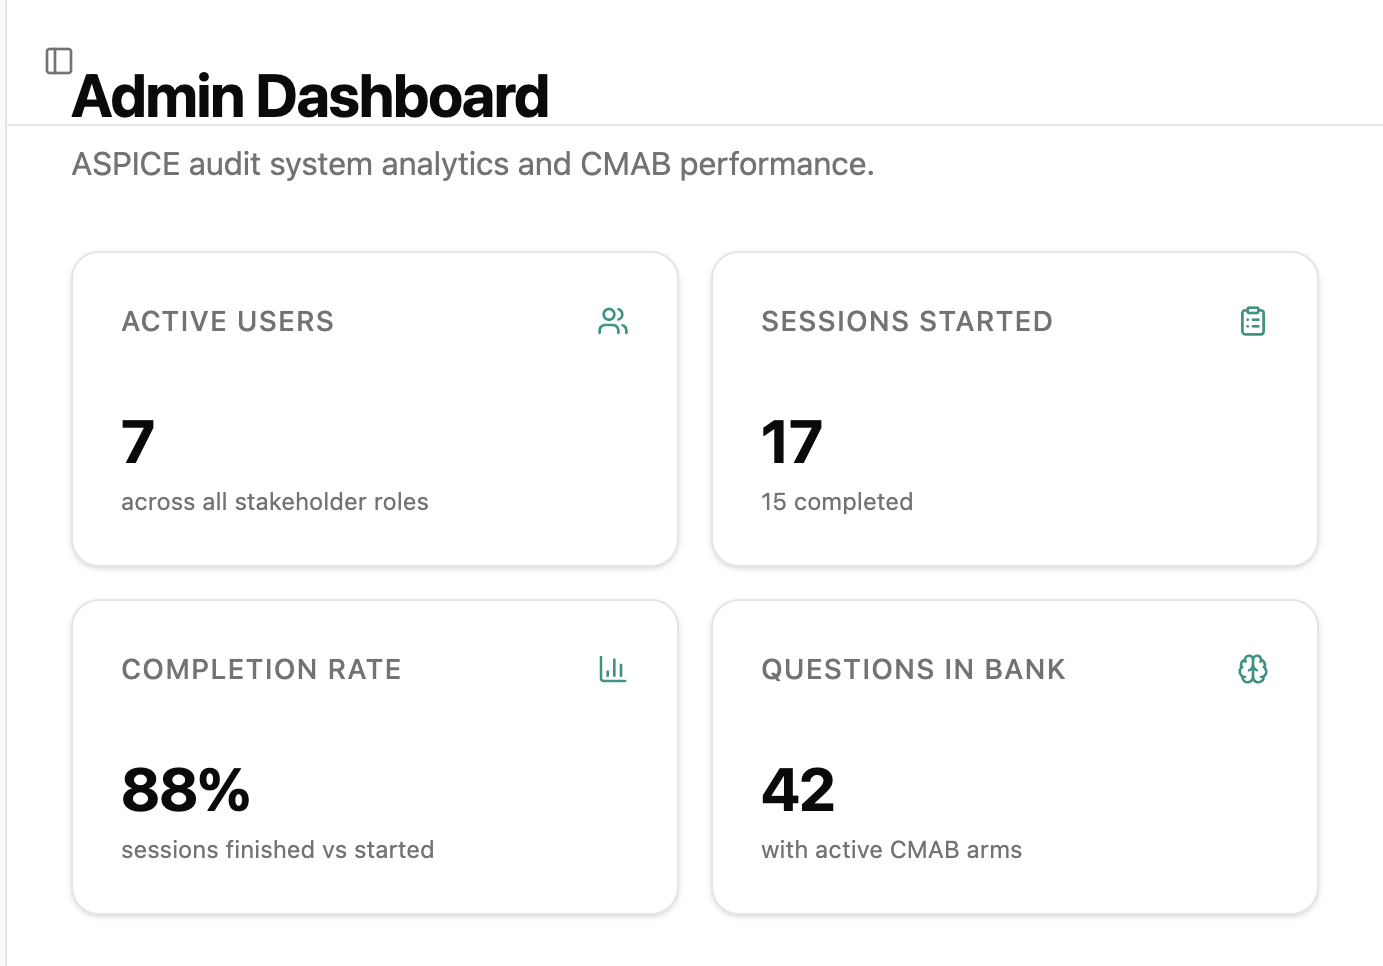
\includegraphics[width=0.75\textwidth]{src/Results_admin_dashboard_numbers.png}
  \caption{Pilot-wide totals, read from the admin dashboard.}
  \label{fig:pilot-dashboard}
\end{figure}

There were 17 sessions started across the seven accounts, with 15 completed and an overall
completion rate of 88\% (Figure~\ref{fig:pilot-dashboard}). Sessions were not all run in one
sitting: the Developer account's own three completed sessions, for example, span from 4 July to
9 September 2026, and the pilot as a whole was carried out over a comparable stretch rather than
all at once. All sessions were conducted the same way as described in
Chapter~\ref{chap:architecture}, with a stakeholder asked a single question at a time from the
42 active questions in the seeded question bank, and a session ending once the eligible pool of
questions was exhausted or the question budget was reached. The only thing that differed between
accounts is which role was signed in, and how that stakeholder responded.

This section is not based on a separate export or manual log, but directly on the participation
table, the CMAB arm statistics, and the overall weakness heatmap, all read live from the
system's own admin analytics endpoints, described in Chapter~\ref{chap:implementation}, the same
ones an administrator would use to monitor the system day to day.

\section{CMAB Behaviour Observed from Real Pilot Sessions}

Now that real data on real usage exists, this section addresses not just what
Chapter~\ref{chap:architecture} says the CMAB engine will do, but what it actually did.

\subsection{Bandit Arm Statistics (Pull Count and Average Reward)}
\label{sec:cmab-arms}

\begin{figure}[h]
  \centering
  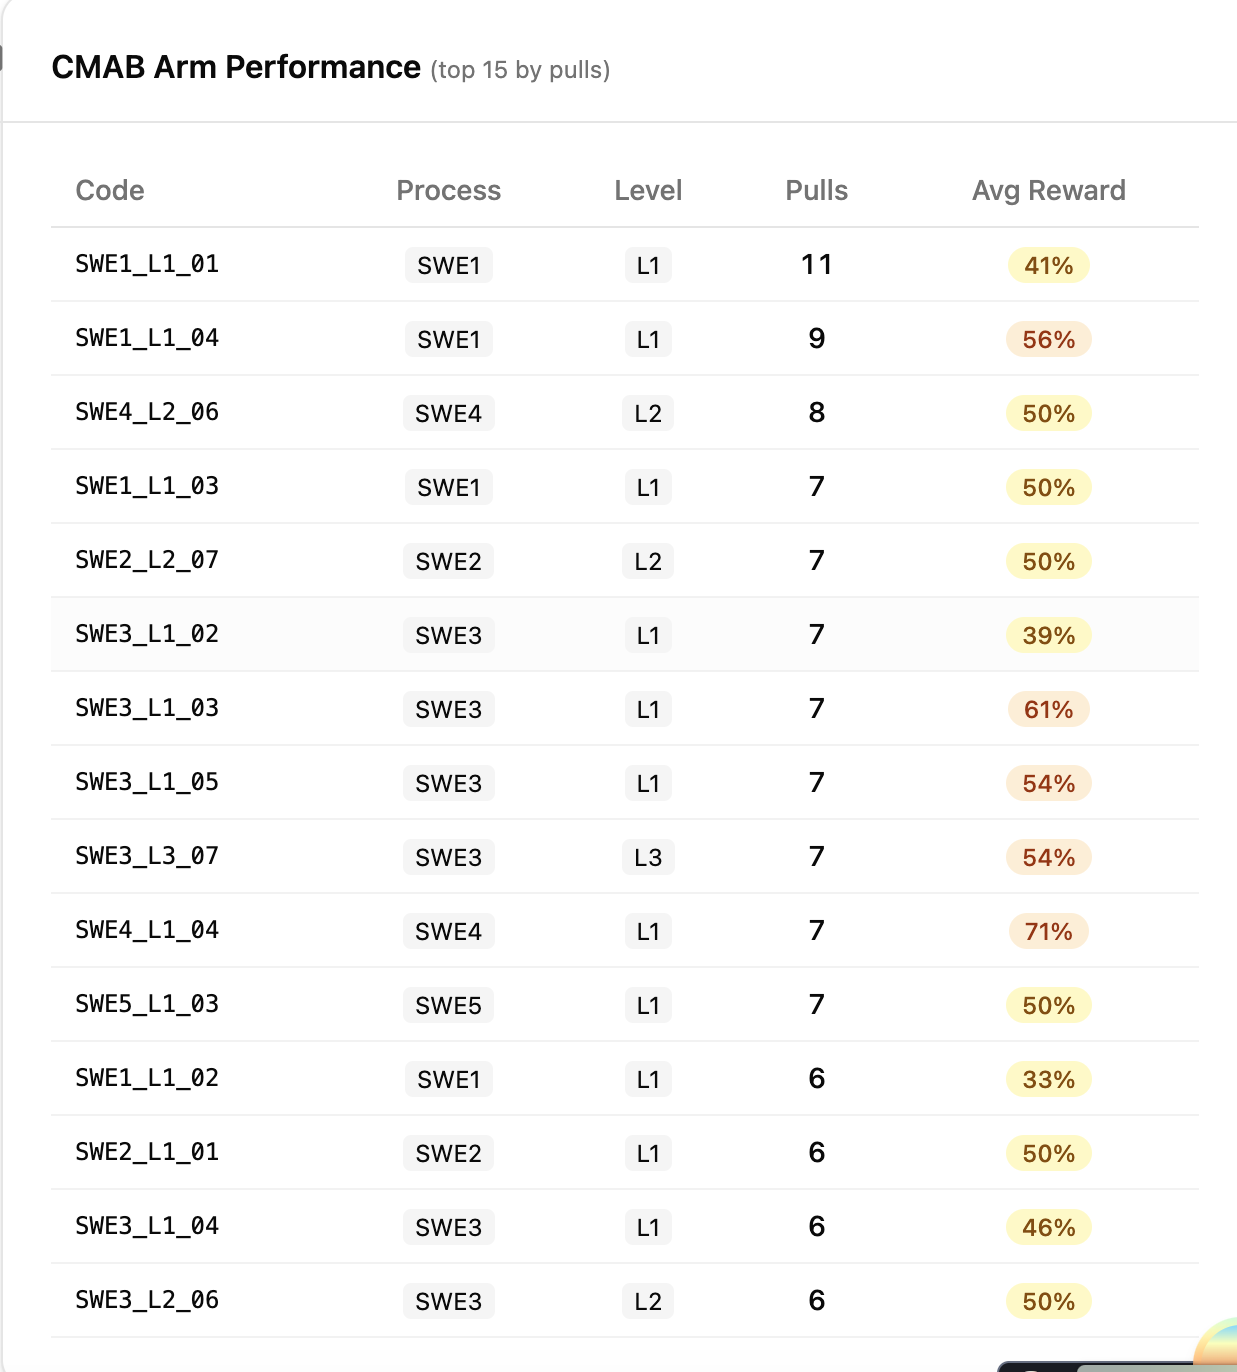
\includegraphics[width=0.8\textwidth]{src/Results_admin_dashboard_cmab.png}
  \caption{The 15 most-pulled questions across the pilot, with pull count and average reward.}
  \label{fig:cmab-arms}
\end{figure}

Figure~\ref{fig:cmab-arms} shows the top 15 questions by pull count, out of the 42 active
questions that make up the seeded bank. Pull counts range from 11 for the most-selected
question, \texttt{SWE1\_L1\_01}, down through single digits for the rest of the top 15;
questions outside this list were pulled less often still. Average reward across these top arms
ranges from 33\% (\texttt{SWE1\_L1\_02}) to 71\% (\texttt{SWE4\_L1\_04}), which shows reward is
not clustering at one extreme: some frequently-asked questions consistently surface weak
answers, and others consistently surface strong ones, which is exactly the signal LinUCB's
$\theta_a^\top x$ term is meant to pick up on.

\texttt{SWE1\_L1\_01} leading the table is not surprising on its own terms: it is also the first
question a brand-new session is ever offered, since every question starts from an identical,
maximally-uncertain arm, and the coverage bonus rewards touching a new process early. What is
more informative is which process dominates the rest of the list: six of the fifteen most-pulled
arms belong to SWE.3, more than any other process, and none belong to SWE.6. That pattern is
consistent with the aggregate weakness heatmap in Section~\ref{sec:aggregate-weakness}: SWE.3
and SWE.4 are the two processes with a significant-gap score at more than one capability level,
and together account for eight of these fifteen most-pulled arms, while SWE.6, compliant or
close to it at every level assessed, accounts for none. Correlation is not causation here, the
classifier scores completed sessions independently of which arm LinUCB happened to select, but
an engine that keeps returning to arms it has learned pay off, on a pilot where the processes it
returns to most are also the ones a separately-computed classifier flags as weakest, is behaving
the way Chapter~\ref{chap:architecture} intended it to.

\subsection{Process Coverage Achieved within the Question Budget}

\begin{figure}[h]
  \centering
  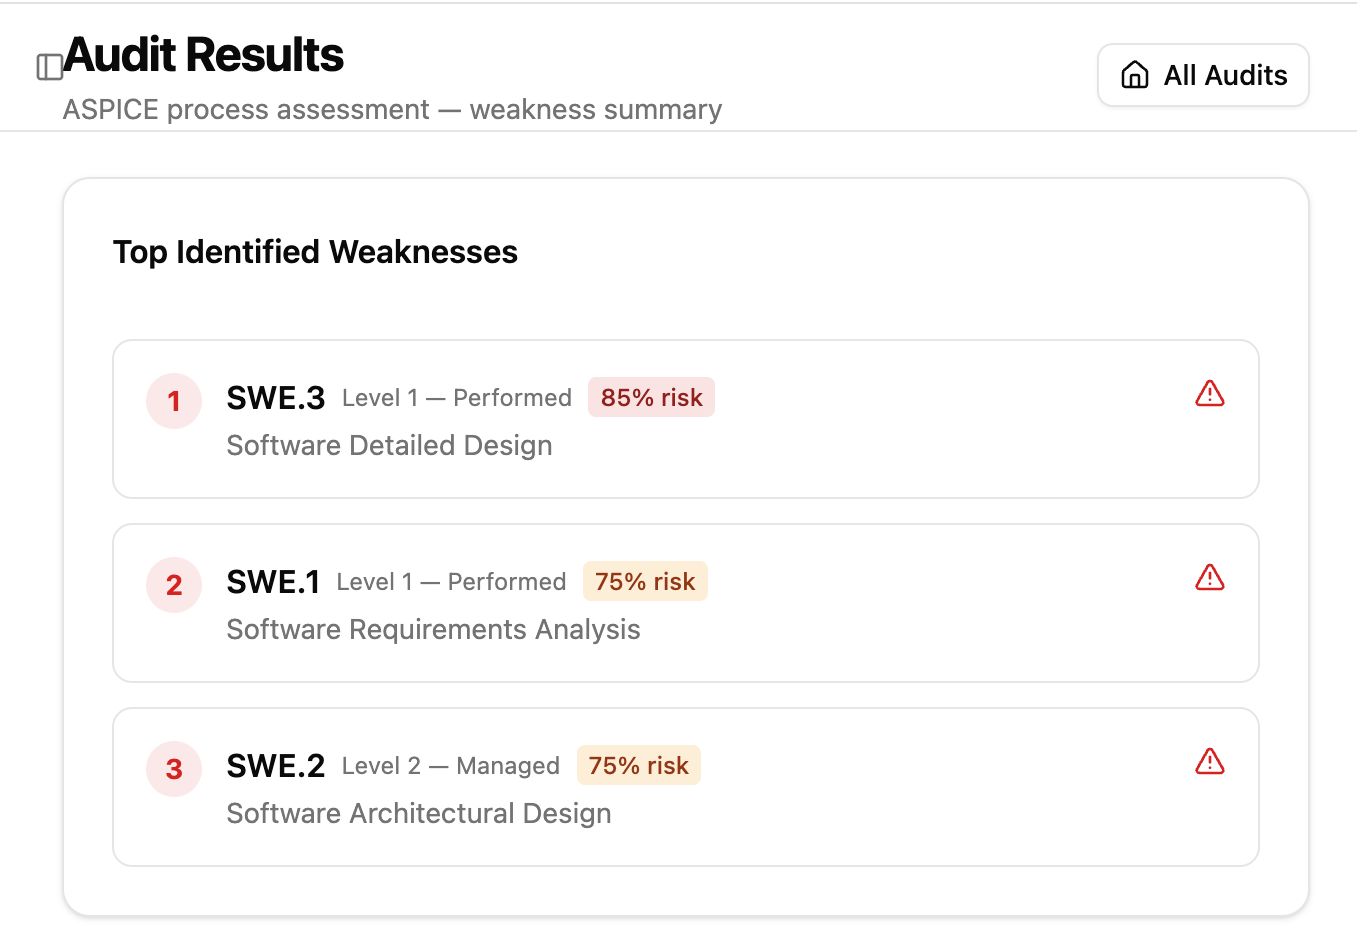
\includegraphics[width=0.8\textwidth]{src/Results_per_session_2.png}
  \caption{Top weaknesses reported for one completed session, run under the ASPICE Assessor
  role.}
  \label{fig:process-coverage}
\end{figure}

A pull-count table on its own does not show whether any single session actually spread across
the six SWE processes, or whether the coverage bonus described in Chapter~\ref{chap:architecture}
is doing its job session by session, not just in aggregate. Figure~\ref{fig:process-coverage}
shows the top three weaknesses reported for one completed session: SWE.3 at Level 1, SWE.1 at
Level 1, and SWE.2 at Level 2. That same session's full radar chart
(Figure~\ref{fig:session-radar}, discussed in Section~\ref{sec:individual-heatmaps}) shows only
four of the six processes touched at all within its question budget, SWE.1 through SWE.4, with
SWE.5 and SWE.6 left unassessed. Within a twelve-question budget and a question bank spanning
six processes at up to three levels each, not every process can realistically be reached in one
sitting; what the coverage bonus is actually doing is making sure the questions that are asked
spread across several processes rather than exhausting the budget on one, which this session
shows happening across four processes rather than one.

\subsection{Repeated Use Across Sessions and Roles}

\begin{figure}[h]
  \centering
  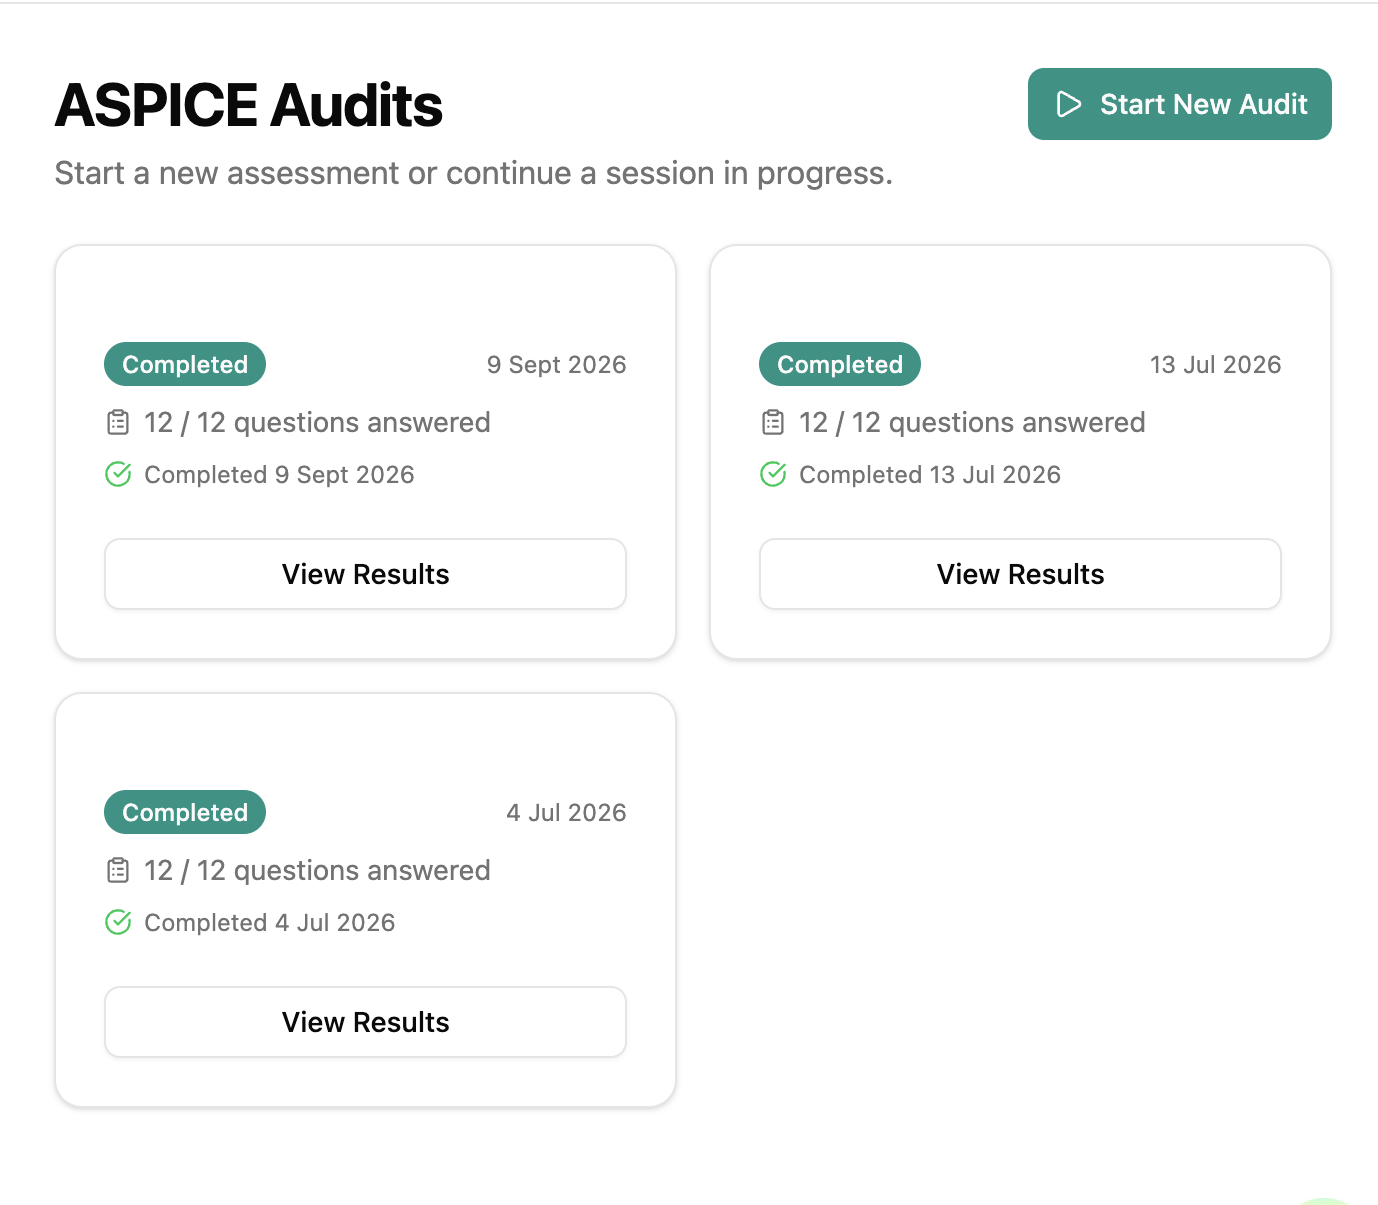
\includegraphics[width=0.8\textwidth]{src/Results_per_completed_session.png}
  \caption{The Developer account's three completed sessions, spanning more than two months.}
  \label{fig:repeated-use}
\end{figure}

The available analytics report pull counts and rewards in aggregate, across every role together,
rather than broken out per role; a genuine per-role comparison of which questions the engine
favours for a Project Manager versus a Test Engineer is left to the larger, externally-recruited
pilot proposed in Chapter~\ref{chap:conclusion}'s future work. What this pilot does show is that
the same account, under the same role, returns to the system and completes further sessions
rather than only ever running one: the Developer account's three completed sessions
(Figure~\ref{fig:repeated-use}) span more than two months, from 4 July to 9 September 2026, each
one drawing on the same shared \texttt{BanditArmState} rows that every other account's sessions
update too. Every session, regardless of role or date, learns from the same continuously-updated
arms, which is the point of keeping bandit state independent of any one session or user, as
Chapter~\ref{chap:architecture} describes it.

\section{Weakness Classification Results from Pilot Sessions}

The functional verification walkthrough exercised the weakness classifier on exactly one
session. This section reports what it produced across all 15 completed pilot sessions.

\subsection{Individual Session Heatmaps and Radar Charts}
\label{sec:individual-heatmaps}

\begin{figure}[h]
  \centering
  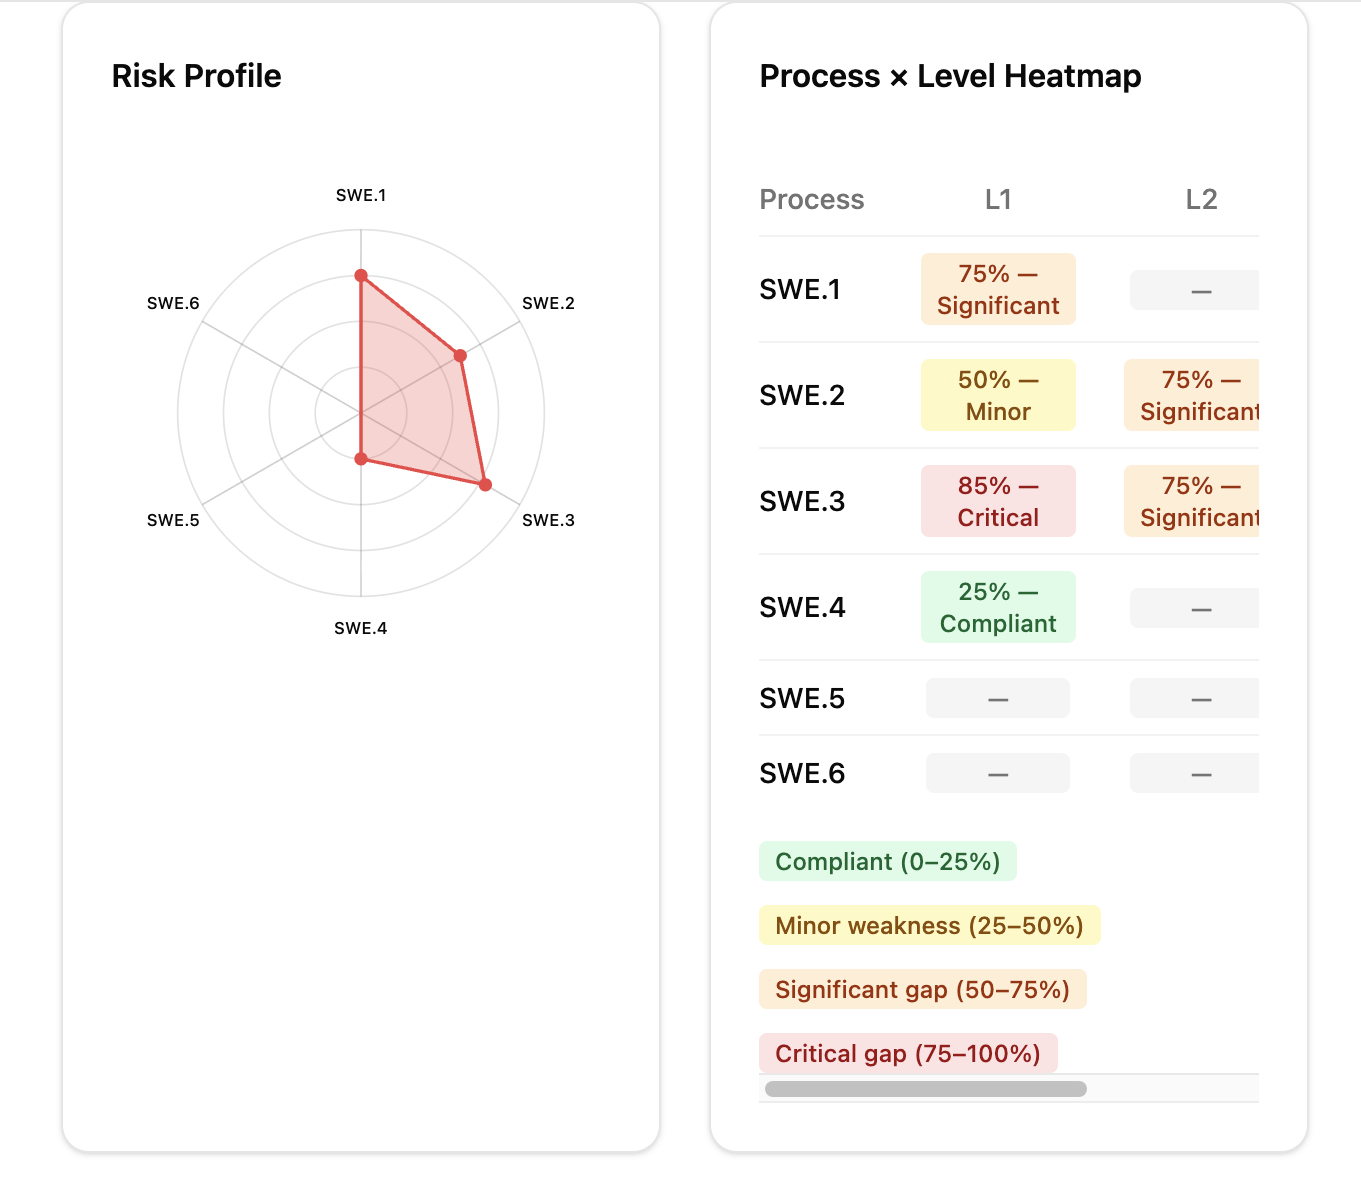
\includegraphics[width=0.8\textwidth]{src/Results_per_session_1.png}
  \caption{One completed session's risk profile and process-by-level heatmap.}
  \label{fig:session-radar}
\end{figure}

Figure~\ref{fig:session-radar} shows one completed session's result in full: a radar chart
across the four processes it actually covered, and the process-by-level heatmap behind it,
coloured by the same four bands from Table~\ref{tab:classification-thresholds}. This session,
run under the ASPICE Assessor role, reported a critical gap at SWE.3 Level 1 (85\%), and
significant gaps at SWE.1 Level 1 (75\%) and SWE.2 Level 2 (75\%). Set against the aggregate
scores for those same three cells, 47\%, 49\%, and 58\% respectively, this one session reads
noticeably worse than the pilot average. SWE.4 Level 1 shows the opposite pattern: this session
scored it 25\%, compliant, while the aggregate across all 15 sessions puts the same cell at 52\%,
a significant gap. Neither number is wrong; they are answering different questions. A stakeholder
finishing this specific session sees a critical warning immediately, not a smoothed-over average
waiting on more data to accumulate, and that immediacy, not agreement with the aggregate, is what
Chapter~\ref{chap:introduction} originally set out to provide.

\subsection{Aggregate Weakness Heatmap and Score Distribution across All Pilot Sessions}
\label{sec:aggregate-weakness}

\begin{figure}[h]
  \centering
  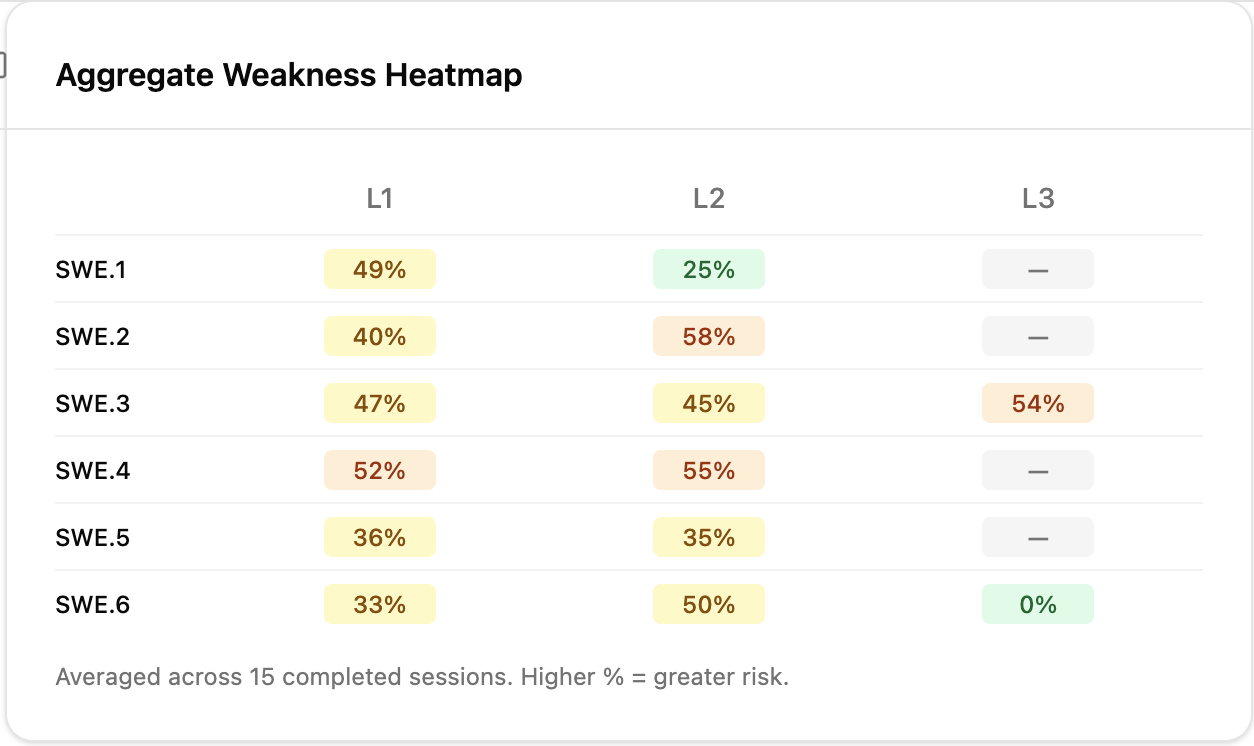
\includegraphics[width=0.8\textwidth]{src/Results_admin_dashboard_weakness_map.png}
  \caption{Weakness scores averaged across all 15 completed pilot sessions.}
  \label{fig:aggregate-heatmap}
\end{figure}

Figure~\ref{fig:aggregate-heatmap} averages every completed session's scores into the same
6-by-3 grid, giving a picture of the whole pilot rather than one session in isolation. No cell
reaches the critical band (75--100\%) at this aggregate level; the highest average scores are
SWE.4 Level 2 (55\%) and SWE.3 Level 3 (54\%), both in the significant-gap band, with the rest
split between minor weakness and, at SWE.1 Level 2 (25\%) and SWE.6 Level 3 (0\%), fully
compliant. SWE.3 and SWE.4 are the only two processes with a significant-gap score at more than
one level, matching the CMAB engine's own pattern of pulling SWE.3 and SWE.4 questions more than
any other process (Section~\ref{sec:cmab-arms}). SWE.6, by contrast, is compliant or close to it
at every level assessed, and was also the process the CMAB engine pulled least. Across a pilot
this size, the engine's selection pattern and the classifier's independent scoring of the same
sessions are telling a consistent story, even though neither computation feeds directly into the
other.

\section{Discussion of Results}

The previous sections cover five different angles on the same system: code quality, whether it
works end to end, who used it and how, what the recommendation engine did, and what the
classifier reported back. Together, they support one central claim more strongly than any single
section does on its own.

The clearest evidence is that two independently-computed things agree. From a completely
separate calculation, the two processes with the highest overall weakness scores are SWE.3 and
SWE.4 (Section~\ref{sec:aggregate-weakness}), and these are also the two processes most
represented among the CMAB engine's most-pulled questions (Section~\ref{sec:cmab-arms}). Neither
number was derived from the other -- pull count comes from LinUCB's own selection history, and
the aggregate score comes from averaging the stakeholder responses -- yet they point in the same
direction. That is real evidence the recommendation engine is behaving as
Chapter~\ref{chap:architecture} designed it to on real, non-simulated data: learning to spend a
session's limited question budget on the processes that actually turn out to be weak, rather
than on whichever process happens to be asked about first.

The second finding worth pulling forward is the gap between one session's result and the
aggregate. Section~\ref{sec:individual-heatmaps} showed a single session scoring SWE.4 Level 1
as compliant (25\%), while the aggregate across the fifteen completed sessions places that same
cell at a significant gap (52\%). Both are correct; they answer different questions, and that
difference is precisely the argument for RQ4: a stakeholder who only ever sees an aggregate
view, updated slowly as sessions accumulate, could easily miss a specific session's critical
finding. Early, per-session visibility is not a redundant feature sitting alongside the
aggregate view -- it is catching something the aggregate view structurally cannot.

This pilot does not resolve the question Chapter~\ref{chap:architecture}'s design decision left
open: whether LinUCB is actually the right algorithm choice compared to $\epsilon$-greedy or
Thompson Sampling. The closest evidence is the simulation in the closest prior work, which
showed $\epsilon$-greedy scoring higher on raw reward (Table~\ref{tab:recommender-results},
Chapter~\ref{chap:sota}). This chapter cannot answer that question, since no alternative
algorithm was implemented or tested against this thesis's own real data; that comparison is left
to Chapter~\ref{chap:conclusion}'s future work. What this pilot does answer is a different, and
in some ways more basic, question: whether the whole mechanism -- the question bank, the
contextual bandit, and the rule-based classifier -- behaves sensibly at all when real people
answer real questions, rather than only in a simulated environment designed to resemble one. On
the evidence gathered here, it does.

\section{Threats to Validity}
\label{sec:threats-to-validity}

Four threats can be named explicitly, rather than as a generic checklist.

The first is internal validity: the author, who built the system, also carried out the pilot,
answering as each of its seven stakeholder roles. A self-administered pilot carries a real risk
of confirmation bias
-- answering the way one thinks a QA Engineer would answer, rather than the way an actual QA
Engineer, with their own specific project and their own specific blind spots, would answer it.
Chapter~\ref{chap:conclusion} already names the pilot's self-administered scope as a limitation;
this is the more precise mechanism behind why that limitation matters.

The second is construct and external validity, and it is the more serious of the two: the
sessions were not run against one fixed, consistent real project. ASPICE questions are only
meaningful against a specific, real piece of software -- a real requirements document, a real
architecture, real test records -- and answering them from general role knowledge instead, as
this pilot did, means the resulting scores measure the author's own perception of what each role
typically struggles with, not the process maturity of any actual project. This is precisely why
Section~\ref{sec:pilot-participants} frames the pilot as a feasibility test of the mechanism
(does question selection, scoring, and reporting behave sensibly end to end) rather than as
evidence about real-world ASPICE compliance: only a study run against one shared, real codebase,
ideally with independent stakeholders, could support the latter claim, and this thesis does not
attempt to.

The third is sample size. After fifteen completed sessions across seven roles, a pattern can be
seen -- the SWE.3/SWE.4 correlation discussed above -- but there is not enough data to trust any
individual question's average reward as a stable estimate; the top-pulled arms in
Section~\ref{sec:cmab-arms} were each selected only six to eleven times.
\texttt{BanditArmState} also keeps learning after every session, so the exact question sequence
reported in this chapter is itself a one-time snapshot: running the same seven-role pilot again
today, against the arms as they now stand, would not reproduce the same sequence of questions,
even though the selection rule itself is deterministic given a fixed state.

The fourth is the correlation raised in the discussion above. That the CMAB engine's most-pulled
questions and the classifier's highest-scoring processes agree is evidence the mechanism works,
but it is not proof: SWE.3 and SWE.4 could simply have more questions, or answer options that
read as more severe regardless of the underlying process's actual state, and either effect would
produce the same pattern without the algorithm having learned anything at all.
Section~\ref{sec:cmab-arms} already flags this as correlation rather than causation; it is
restated here as a threat because it bears directly on how much weight RQ2's evidence can carry.

\section{Chapter Summary}

This chapter tested the system against real usage rather than simulation, across five angles:
the backend's own test suite and static analysis, a manual walkthrough confirming the
application works end to end, a self-administered pilot spanning every stakeholder role, what
the CMAB engine actually selected once real answers came back, and what the weakness classifier
reported from those same sessions. Taken together, this evidence demonstrates that the system
works as a proof of concept: a real question bank was actually seeded and served, a
recommendation engine selected questions in a pattern that agrees with an
independently-computed weakness score, a classifier produced a result from real answers to real
questions, and a dashboard displayed that result to a real stakeholder the moment a real session
finished. This is evidence that the mechanism functions end to end on real data, not evidence
that its output is an accurate ASPICE rating: as the threats above make explicit, the agreement
between engine and classifier is correlational rather than proven causal, and the pilot's
self-administered, project-agnostic design means the four research questions are answered at
the level of technical feasibility, not of validated real-world assessment accuracy.

None of this is presented as final. The pilot is real but modest, the algorithm comparison
remains to be done, and the threats named above are stated rather than resolved.
Chapter~\ref{chap:conclusion} takes up exactly that: what these results answer, what they leave
open, and where the system goes from here.\footnote{I used AI tool in this Chapter as a
verification aid, in the same way and for the same purpose as in Chapter~\ref{chap:implementation}.
See the AI Referencing section on page~\pageref{app:ai-referencing} for full details.}

\chapter{Conclusion and Future Work}
\label{chap:conclusion}
% \input{src/conclusion}

This chapter concludes this research by summarising the aims and motivation of the thesis. It
starts with a brief review of the work presented in the preceding chapters, and directly
addresses each of the four research questions presented in Chapter~\ref{chap:introduction}. It
also takes into account the limitations of the system as it stands, and finally gives a list of
suggestions for future research along with some final remarks.

\section{Summary of Contributions}

In Chapter~\ref{chap:introduction}, six contributions were outlined, corresponding to the four
research questions. This section reviews what was actually provided for each.

Chapter~\ref{chap:architecture} developed a structured ASPICE SWE.1--SWE.6 question bank with
each question mapped to a specific base practice and specific roles assigned to each question,
as well as weighted answer options, and Chapter~\ref{chap:implementation} then seeded the bank
with 60 questions and 300 answer options across all six processes.

For RQ2, Chapter~\ref{chap:architecture} built a recommendation engine based on CMAB and LinUCB,
which selects a small number of well-targeted questions per session from a session-state context
that includes the stakeholder role, progress, and coverage of process and capability so far, and
Chapter~\ref{chap:implementation} implemented this engine directly in code, and
Chapter~\ref{chap:results} observed its operation on the deployed system.

For RQ3, Chapter~\ref{chap:architecture} created a rule-based weakness classifier that scores
each assessed (process, capability level) cell without the need for a labelled training set or
judgement by a human assessor, and Chapter~\ref{chap:implementation} implemented it, but in
Chapter~\ref{chap:results} it was used on a real, non-simulated session, not just on the worked
example used in Chapter~\ref{chap:architecture}.

In Chapter~\ref{chap:architecture}, the results dashboard was designed to give early visibility
of weakness classifications for each SWE process; it was built in
Chapter~\ref{chap:implementation}; and finally, the functional verification walkthrough in
Chapter~\ref{chap:results} demonstrated it end to end with a real completed session.

There are two contributions above these four. The first is the whole web application itself,
described in Chapters~\ref{chap:architecture} and~\ref{chap:implementation}: FastAPI, React, and
PostgreSQL tied together end to end, which is what let the other four be evaluated on a working
system, rather than just on paper. The second is the evaluation itself: Chapter~\ref{chap:results}
evaluated the system in real, non-simulated sessions, whereas neither supervisor paper did
(Chapter~\ref{chap:sota}).

\section{Answering the Research Questions}

\textbf{RQ1.} How do the ASPICE SWE.1--SWE.6 base practices get converted to a structured,
weighted question bank of auditor-style questions? The solution, which is explored in
Chapter~\ref{chap:architecture} and implemented in Chapter~\ref{chap:implementation}, is to turn
each base practice into a question for the stakeholder to answer about their own work, not
something for an assessor to check off a list. Then five answer options are attached, in order
from best practice to none at all, and each option is given a weight. Each question has also
been assigned the stakeholder roles that can provide meaningful answers, and the base practice
it falls under. This was applied to SWE.1--SWE.6, and yielded the 60-question, 300-option bank
of Chapter~\ref{chap:implementation}.

\textbf{RQ2.} How can a web-based recommendation system reduce the question bank to a handful of
well-targeted questions per session? LinUCB does this by assigning a score to each eligible
question based on a context vector that represents the stakeholder's role and the state of the
session up to that point, then choosing the best-scoring question at each turn and adjusting its
estimate after each response. This is not just an abstract engine, but one
Chapter~\ref{chap:results} confirmed running end to end on a real session on the deployed
system.

\textbf{RQ3.} How can stakeholder answers be automatically classified into a process weakness
rating without relying on a human assessor's judgement? The weakness classifier does so by
taking the normalised weight of each answer in each (process, capability level) cell that the
session actually covered, assigning a score to each cell in one of four bands, and ranking the
weakest cells. This is a rule that is fixed at design time and is not learned from labelled
data, so there is no need for an assessor's input at run time. In Chapter~\ref{chap:results},
this classifier was applied to a real submitted session and confirmed to produce a stored
result automatically.

\textbf{RQ4.} How can these results be communicated so that weaknesses are apparent early on,
rather than only at the next scheduled audit? Through the results dashboard, as described in
Chapter~\ref{chap:architecture} and built in Chapter~\ref{chap:implementation}: a radar chart, a
process-by-level heatmap, and a ranked list of the top weaknesses with recommendations,
generated at the end of a session, not at the next scheduled audit. This is demonstrated in the
walkthrough of a real completed session in Chapter~\ref{chap:results}.

\section{Limitations}

There are some shortcomings to this system worth pointing out. It is limited in scope, as
defined in Chapter~\ref{chap:introduction}: the Software Engineering process group, SWE.1 to
SWE.6, and only capability levels L1 to L3. ASPICE is rarely used on an individual process group
basis. The complete process reference model, described in Chapter~\ref{chap:background},
consists of eleven process groups: Acquisition, Supply, System Engineering, Software
Engineering, Hardware Engineering, Machine Learning Engineering, Validation, Supporting Process,
Management, Process Improvement, and Reuse. A real assessment may need to take several of these
process groups into account. For instance, the software requirements of SWE.1 are derived from
SYS-level system requirements, and a number of SWE base practices depend on SUP processes for
configuration management and quality assurance evidence. A system that only asks about
SWE.1--SWE.6 cannot be aware of this context, and a project that appears weak from the SWE point
of view alone may turn out to be stronger, or weaker, once System Engineering or Supporting
processes are taken into account. For a similar reason, there is no way to reach capability
levels L4 and L5 in a single stakeholder-reporting session, regardless of how the session is
designed: these levels rely on quantitative process control and organisation-wide improvement,
achieved only over the course of many projects and over time, which is structurally beyond what
a single stakeholder can report in a single session.

The weakness classifier assumes that the capability level was assigned to each question
correctly by whoever created the question bank. A more faithful interpretation of how ASPICE
derives a capability level, based on the pattern of process-attribute ratings rather than a
single pre-assigned rating, is left as a system-derived redesign for Future Work.

The question bank and its mapping of answers to weights have not been verified by a certified
ASPICE assessor. The question wording, and the mapping of answers to weights, are taken from the
published PAM, but are not necessarily the same as would be produced by a qualified person
conducting a real ASPICE assessment. A professional auditor may well ask a different question,
give a different weight to an answer choice, or decide that a base practice's wording in this
thesis understates or overstates a particular aspect of the practice as it is typically
evaluated in industry. Until that check is completed, the system's output is best treated as a
structured, consistent signal rather than a certified rating. The authenticity of each
individual question, that is, whether it matches how a real assessor would actually probe that
base practice, has not been independently verified.

The evaluation in Chapter~\ref{chap:results} is real, not simulated, but the number of
stakeholder-role accounts it was run on is limited, and the learned state of the CMAB engine
reflects only that level of usage. As mentioned in Chapter~\ref{chap:introduction}, the answer
weights were inspired by, but not validated against, expert interviews.

There are also gaps in test coverage. The automated tests cover only the core services and the
surrounding signup and login pages, not every scenario and edge case a production system would
eventually need. No automated end-to-end test exists for the actual audit flow, starting a
session, answering a question, and viewing results; this was verified manually instead, as
described in Chapter~\ref{chap:results}.

Even within the process groups that are included, a few ASPICE concepts are not captured by a
multiple-choice question bank. Work product review is a key element of ASPICE assessment, in
which the assessor reads the actual requirements document, the actual test report, the actual
architecture model, and judges the process from that evidence directly. This system instead
asks a stakeholder to describe their own work in multiple-choice form, which is a self-report
rather than an independent review of the artifact itself, and carries the usual risks of
self-reporting: a stakeholder may misjudge, round up, or simply not know how their own
requirements document actually reads against the base practice being asked about. Generic
practices and generic resources, which ASPICE uses to rate capability levels L2 and above across
every process the same way, are not represented as their own questions; instead, they are folded
into the same per-process weighting already used for base practices, rather than assessed
separately the way the standard itself treats them. Finally, ASPICE's own rating scale, Not
achieved, Partially achieved, Largely achieved, and Fully achieved, each tied to a corresponding
range of evidence found, is compressed here into four bands of weakness based on an average of
the answer weights. The mapping between the two is reasonable but not one-to-one, and this
thesis does not claim the two scales agree in every case.

\section{Future Work}
\subsection{Larger-Scale Pilot with Certified ASPICE Assessors}

The pilot in Chapter~\ref{chap:results} was conducted by the author with a few stakeholder-role
accounts. A natural next step is a larger pilot with real, independent participants from a
number of projects, ideally with certified ASPICE assessors comparing the system's output
against their own manual assessment of the same project. This would test something the current
pilot cannot: whether the weakness classifier's automatic rating agrees with the judgement of an
experienced assessor working from the same evidence.

\subsection{Corroborating Self-Reported Answers with Work-Product Evidence}

Each answer in this system is a stakeholder's characterisation of their own work, not an
assessor's interpretation of the requirements document, test report, or architecture model the
answer actually refers to. A stakeholder might be mistaken, or round up, without intending to. A
future version could have a stakeholder attach or link the specific work product a question is
about when answering it, giving the self-report something to be checked against, rather than
standing on its own.

\subsection{Simulation-Based Benchmarking of LinUCB against Baselines}

The decision to use LinUCB instead of $\epsilon$-greedy and Thompson Sampling was not made based
on raw reward, but on other reasons stated in Chapter~\ref{chap:architecture}, noting that
$\epsilon$-greedy outperformed LinUCB in simulation. A direct comparison of the three algorithms
against this thesis's own question bank and context vector, rather than the simulated benchmark
from the prior paper, would reveal whether that gap holds, narrows, or widens when measured
against this thesis's own question bank instead of the prior paper's.

\subsection{Supervised Weakness Classifier from Accumulated Sessions}

Because there is no labelled training data, the weakness classifier is a fixed rule rather than
a learned one. After a sufficient number of sessions, a supervised classifier could be trained on
assessor-validated labels instead of, or alongside, the current rule-based average, potentially
detecting patterns between questions that a simple per-cell average would miss. This becomes
feasible at around fifty or more sessions; with fewer, such a model would likely overfit to a
handful of examples.

\subsection{Expert/Assessor-Validated Reward Signal}

The weights behind both the CMAB's reward and the classifier's scores were not validated for
this thesis's own question bank, but were instead taken from the closest prior work, where they
had been validated through expert interviews. The weights used here would need to be validated
with automotive ASPICE experts, as was done in that prior work, to determine whether they
actually reflect real-world severity.

\subsection{Expansion to Additional ASPICE Process Groups}

This thesis deals only with the Software Engineering process group. The same technique, base
practices turned into weighted questions, selection by a CMAB engine, and scoring by a
rule-based classifier, can be applied directly to System Engineering, Management, and Supporting
processes. This is not only a hypothetical extension: a concurrent thesis in the same department
applies the same approach to the System Engineering process group,
SYS.1--SYS.6~\cite{zargham2026sys}. Combining that work with this one would let a single system
give a fuller picture of a project's ASPICE capability than either a software engineering or a
system engineering slice alone.

\subsection{Extending to Capability Levels L4 and L5}

Capability levels L4 and L5 are not included in this thesis, since they rely on quantitative
process control and organisation-wide improvement gained over many projects, not the evidence of
a single session. Once enough sessions accumulate across many projects in the same organisation,
though, that evidence does begin to exist: over time, the weakness results are themselves a
quantitative record of a process's performance across projects. These could be rolled up into
the kind of process-performance baseline L4 asks for, and monitored for the improvement trends
L5 calls for. This would require extending the classifier to read across sessions and projects,
rather than scoring one session at a time as it currently does.

\subsection{Modeling Generic Practices and Aligning with the ISO 33020 Rating Scale}

This thesis combines every question into a single per-process weighting, regardless of whether
the base practice it refers to sits at L1 or is one of the generic practices ISO 33020 uses to
rate L2 and above. A more faithful design would model generic practices and generic resources as
their own question type, scored and reported separately from base practices the way the
standard itself separates them, and would calibrate the four-band weakness classification
against ASPICE's own percentage-based Not achieved, Partially achieved, Largely achieved, Fully
achieved scale, rather than an independently chosen set of thresholds. Both changes would bring
the system's capability rating closer to what a certified assessor would actually produce, at
the cost of a larger question bank and a more complicated scoring model.

\section{Final Remarks}

This thesis started with a particular problem: ASPICE assessment gives a rating only at audit
time, but not at any point in between. A flaw not discovered the week after an audit may go
unnoticed for months, and by the time it is caught, at a follow-up audit or as a downstream
defect, it is far more costly to correct than if it had been caught early. The aim of this
thesis was therefore to investigate whether the SWE.1--SWE.6 base practices could be made
available for stakeholders to check regularly, instead of only when an assessor is present on
site.

This research gives an answer -- a particular mechanism, not just an argument. The question bank
is structured, so that every question is tied to a named base practice and a weighted answer,
and a session's raw answers can be turned into a number without further interpretation. A
contextual multi-armed bandit, LinUCB, adapts to the session and the stakeholder by asking
fewer, more relevant questions, instead of working through a fixed questionnaire. The answers
that come back are then turned into a weakness rating, per process and per capability level, by
a rule-based classifier, without needing human judgement or a labelled training set. Finally, a
results dashboard displays that rating to a stakeholder immediately once a session has
concluded, rather than at the next scheduled audit.

This thesis is not about a concept, it is a real, deployed system that works. The two supervisor
papers this thesis builds on proposed the same underlying idea and demonstrated it by
simulation; this thesis implements it, runs it, and evaluates it on sessions of a working web
application, at whatever scale the pilot in Chapter~\ref{chap:results} was able to reach. This
thesis fills the space between a simulated proposal and a working system a stakeholder can
actually sign into and use. It is a narrower space than it might sound, too: a modest pilot, a
question bank not yet reviewed by a certified assessor, and a few implementation gaps, all named
clearly earlier in this chapter.

\newpage
None of that narrowness takes away from what was built. The system answers each of its four
research questions with working code and a real result, rather than simply proposing how one
might be achieved, and the limitations recorded here are the kind that come from actually
building and running something, rather than from never having tried. Closing the larger gap,
from a modest, self-administered pilot to the kind of large-scale, assessor-validated deployment
outlined in this chapter's future work, is left for whoever takes this forward next, possibly
the author included. If ASPICE assessment is ever to move from a periodic audit towards
something closer to continuous feedback, a system like this one, tested, imperfect, and honest
about where it still falls short, is a reasonable place to start.

%---------------------------------------------------------
% bibliography based on Springer Design
%---------------------------------------------------------

\bibliographystyle{splncs03}
\bibliography{bibliography}

%---------------------------------------------------------
% AI Referencing
%---------------------------------------------------------

\addchap*{AI Referencing}
\label{app:ai-referencing}

This thesis made limited use of AI tools. Where used, this is documented below: which tool, where
in the thesis, and for what purpose.

\begin{description}
  \item[Claude (Anthropic)] Used in Chapter~\ref{chap:implementation} and
  Chapter~\ref{chap:results} as a verification aid, to compare the implementation and evaluation
  described in the text against the actual functionality of the deployed system.
  \item[Claude Design (Anthropic)~\cite{anthropic_claude_design}] Used to generate diagrams
  referenced throughout Chapter~\ref{chap:architecture} and Chapter~\ref{chap:implementation};
  see each diagram's caption for the individual citation.
\end{description}

%---------------------------------------------------------
% Appendices
%---------------------------------------------------------

\appendix
\part*{Appendix}

\chapter{ASPICE Question Bank}
\label{app:questionbank}
Full list of the 60 questions and 300 options used in the seeded question bank, covering
SWE.1--SWE.6. The full bank is reproduced here as screenshots of the source question-bank
document (\texttt{Detailed\_question\_analysis\_clean.md}), one figure per SWE process.

\section*{Legend}

\begin{center}
\rowcolors{2}{green!5}{white}
\begin{tabular}{c l}
\toprule
\rowcolor{green!55!black}
\thw{Weight} & \thw{Meaning} \\
\midrule
0 & Best / lowest risk \\
5 & Worst / highest risk (highest CMAB reward) \\
\bottomrule
\end{tabular}
\end{center}

\begin{center}
\rowcolors{2}{green!5}{white}
\begin{tabular}{c l}
\toprule
\rowcolor{green!55!black}
\thw{Code} & \thw{Stakeholder} \\
\midrule
SD  & Software Developer \\
SA  & Software Architect \\
PM  & Project Manager \\
QA  & QA Engineer \\
TE  & Test Engineer \\
TL  & Team Lead \\
ASR & ASPICE Assessor \\
\bottomrule
\end{tabular}
\end{center}

\begin{center}
\rowcolors{2}{green!5}{white}
\begin{tabular}{c l}
\toprule
\rowcolor{green!55!black}
\thw{Level} & \thw{Meaning} \\
\midrule
L1 & Performed \\
L2 & Managed \\
L3 & Established \\
\bottomrule
\end{tabular}
\end{center}

\section*{SWE.1: Software Requirements Analysis}

\begin{center}
  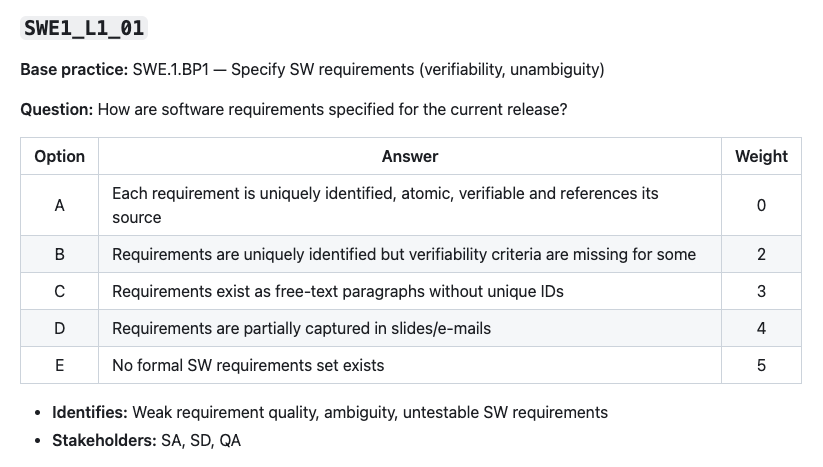
\includegraphics[width=0.95\textwidth,height=0.3\textheight,keepaspectratio]{src/Q1.png}\\[0.3cm]
  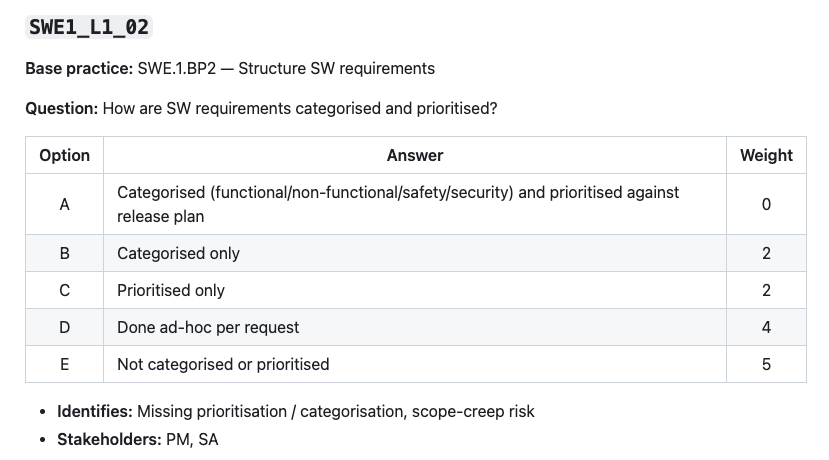
\includegraphics[width=0.95\textwidth,height=0.3\textheight,keepaspectratio]{src/Q2.png}\\[0.3cm]
  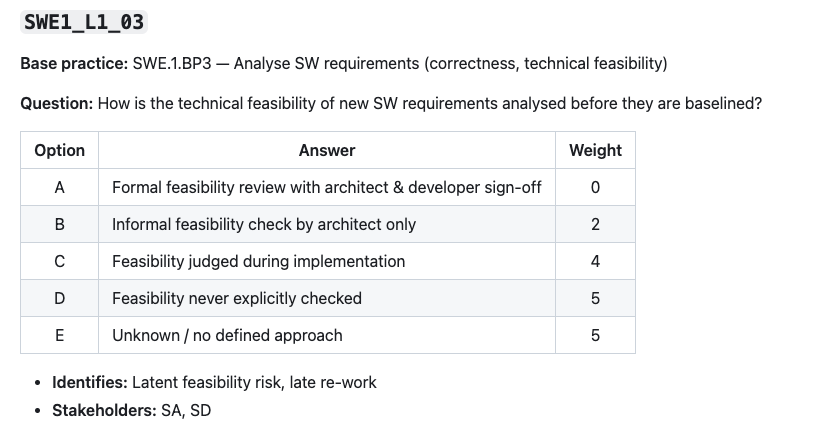
\includegraphics[width=0.95\textwidth,height=0.3\textheight,keepaspectratio]{src/Q3.png}\\[0.3cm]
  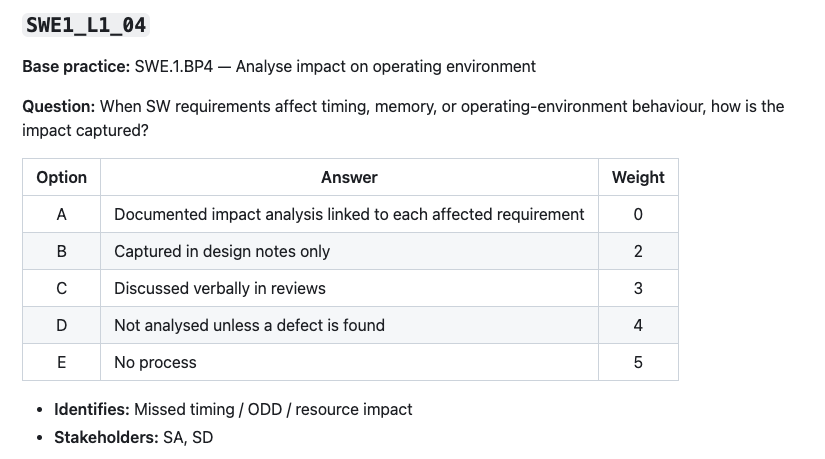
\includegraphics[width=0.95\textwidth,height=0.3\textheight,keepaspectratio]{src/Q4.png}\\[0.3cm]
  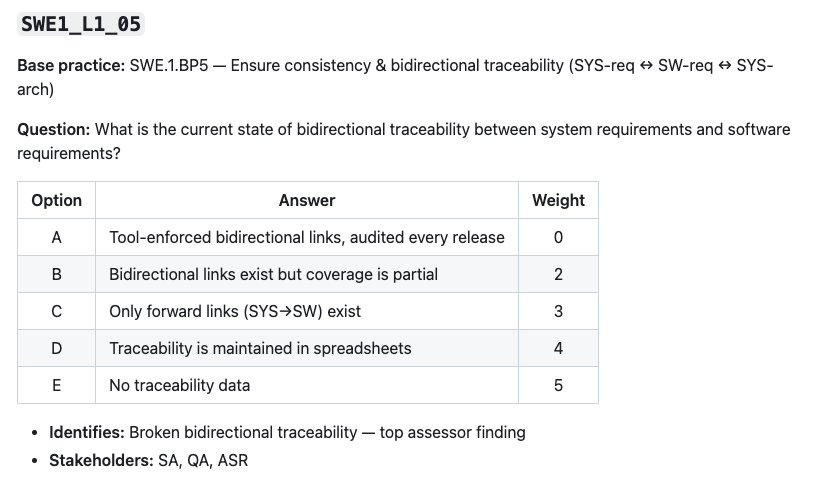
\includegraphics[width=0.95\textwidth,height=0.3\textheight,keepaspectratio]{src/Q5.png}\\[0.3cm]
  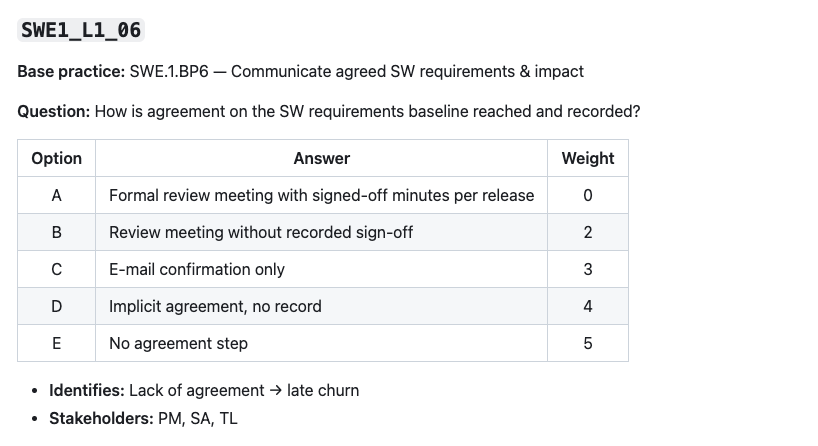
\includegraphics[width=0.95\textwidth,height=0.3\textheight,keepaspectratio]{src/Q6.png}\\[0.3cm]
  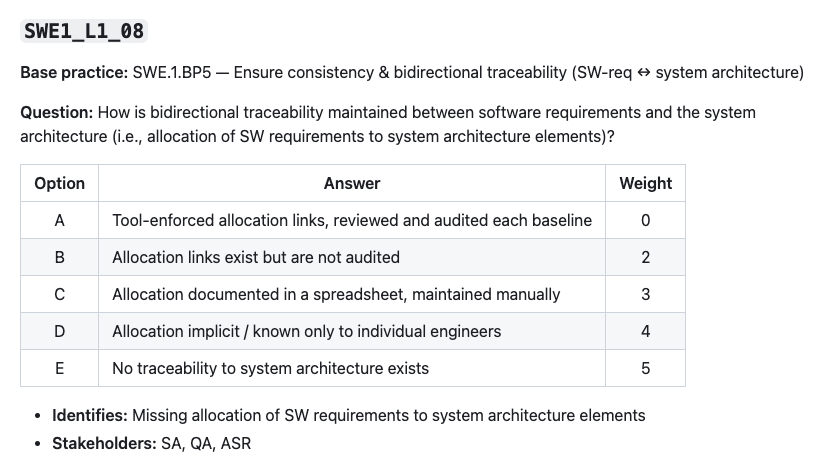
\includegraphics[width=0.95\textwidth,height=0.3\textheight,keepaspectratio]{src/Q7.png}\\[0.3cm]
  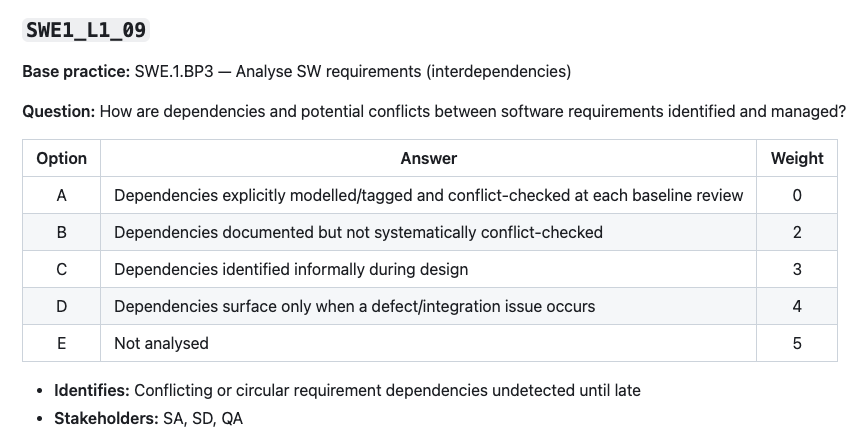
\includegraphics[width=0.95\textwidth,height=0.3\textheight,keepaspectratio]{src/Q8.png}\\[0.3cm]
  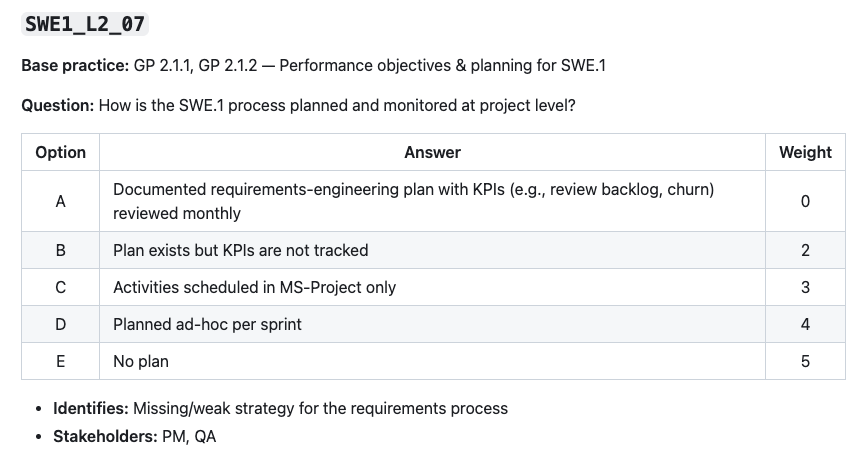
\includegraphics[width=0.95\textwidth,height=0.3\textheight,keepaspectratio]{src/Q9.png}\\[0.3cm]
  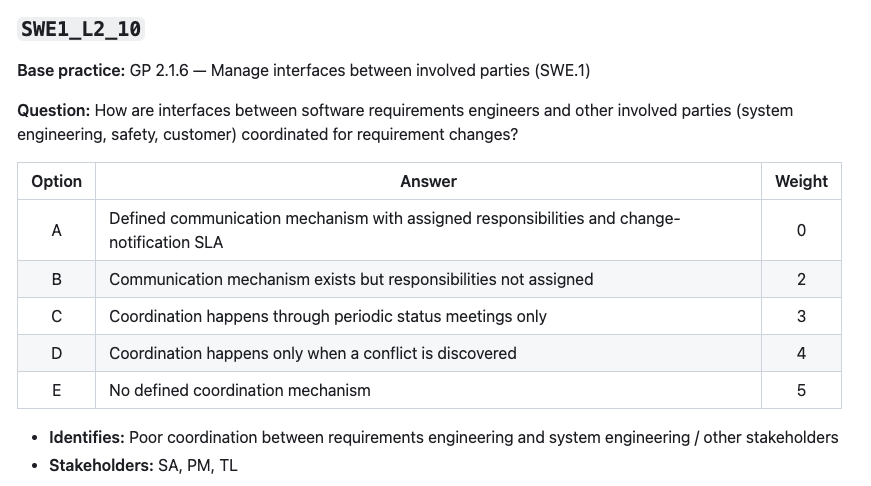
\includegraphics[width=0.95\textwidth,height=0.3\textheight,keepaspectratio]{src/Q10.png}\\[0.3cm]
  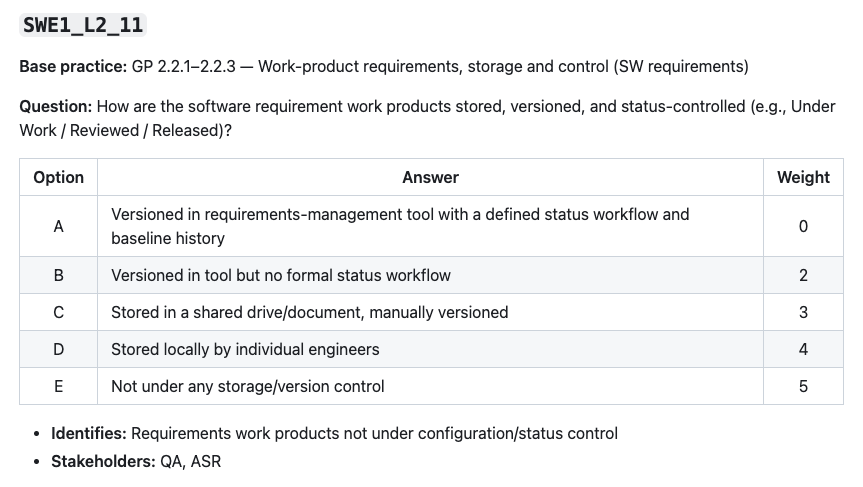
\includegraphics[width=0.95\textwidth,height=0.3\textheight,keepaspectratio]{src/Q11.png}\\[0.3cm]
  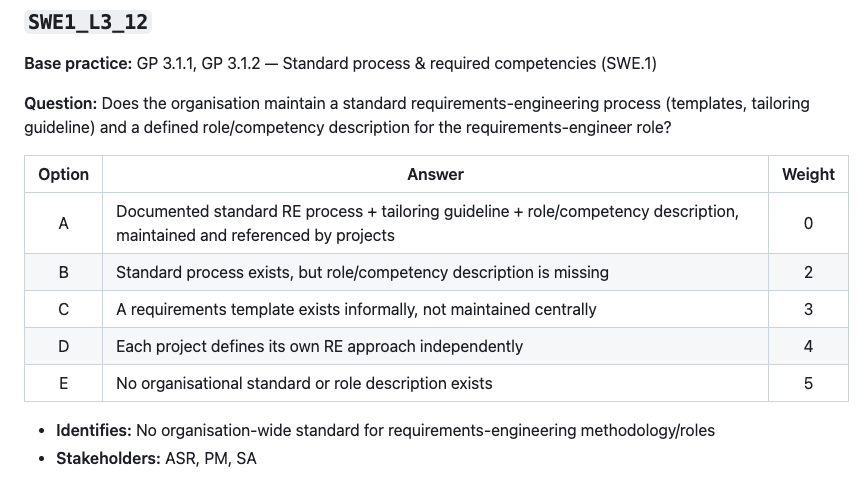
\includegraphics[width=0.95\textwidth,height=0.3\textheight,keepaspectratio]{src/Q12.png}
\end{center}

\section*{SWE.2: Software Architectural Design}

\begin{center}
  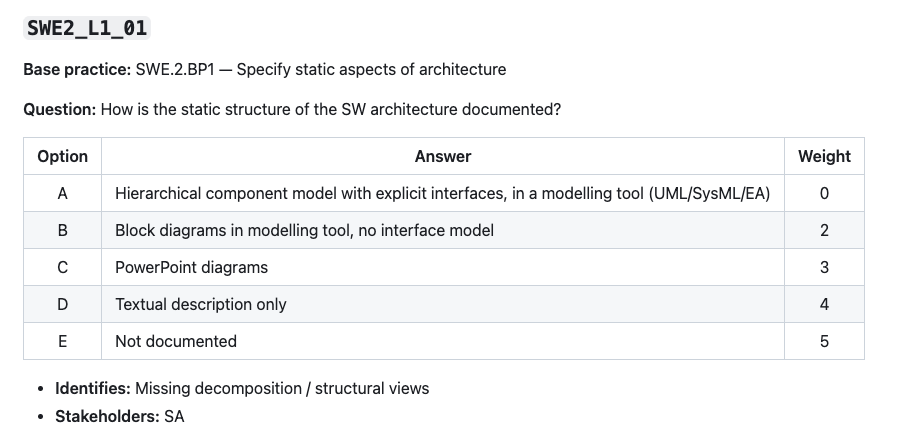
\includegraphics[width=0.95\textwidth,height=0.3\textheight,keepaspectratio]{src/Q13.png}\\[0.3cm]
  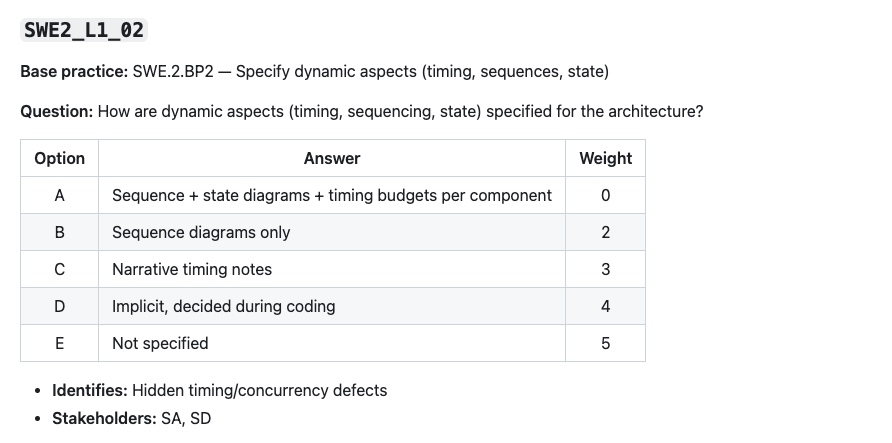
\includegraphics[width=0.95\textwidth,height=0.3\textheight,keepaspectratio]{src/Q14.png}\\[0.3cm]
  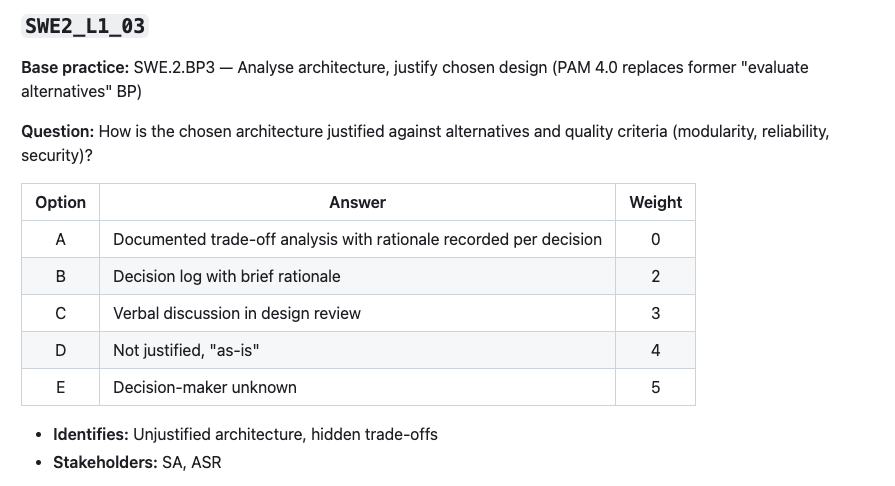
\includegraphics[width=0.95\textwidth,height=0.3\textheight,keepaspectratio]{src/Q15.png}\\[0.3cm]
  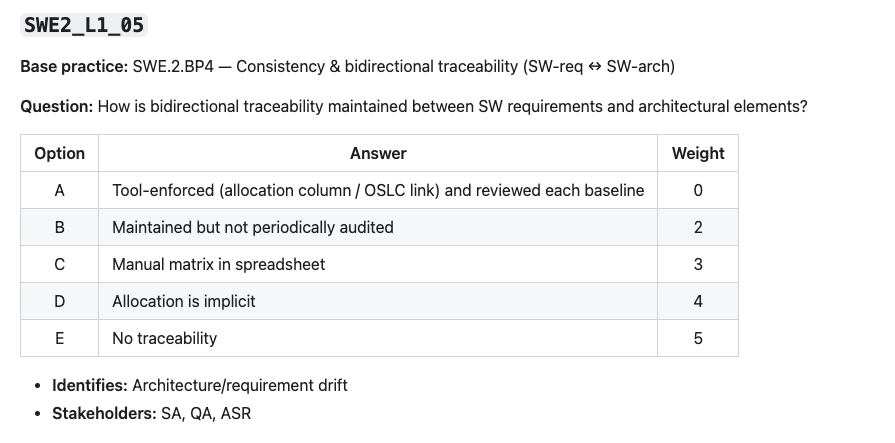
\includegraphics[width=0.95\textwidth,height=0.3\textheight,keepaspectratio]{src/Q16.png}\\[0.3cm]
  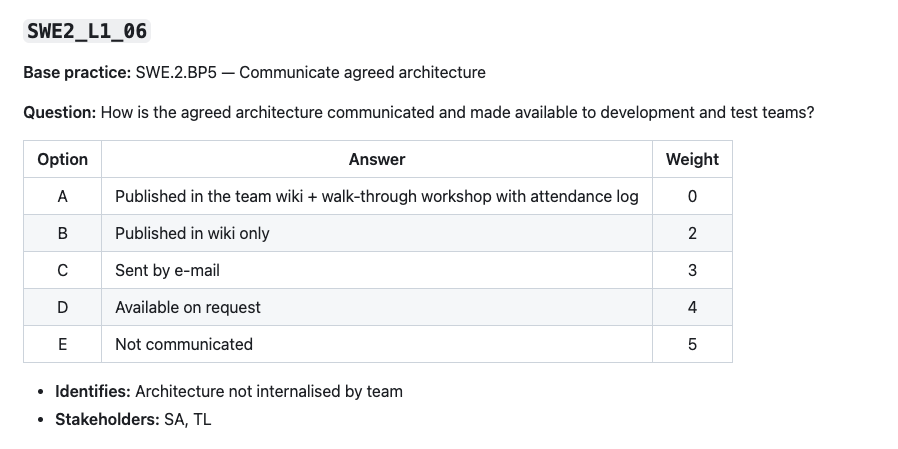
\includegraphics[width=0.95\textwidth,height=0.3\textheight,keepaspectratio]{src/Q17.png}\\[0.3cm]
  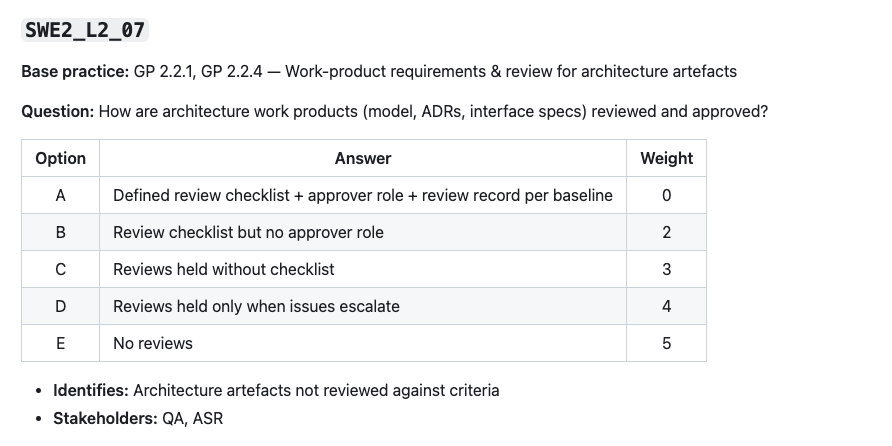
\includegraphics[width=0.95\textwidth,height=0.3\textheight,keepaspectratio]{src/Q18.png}\\[0.3cm]
  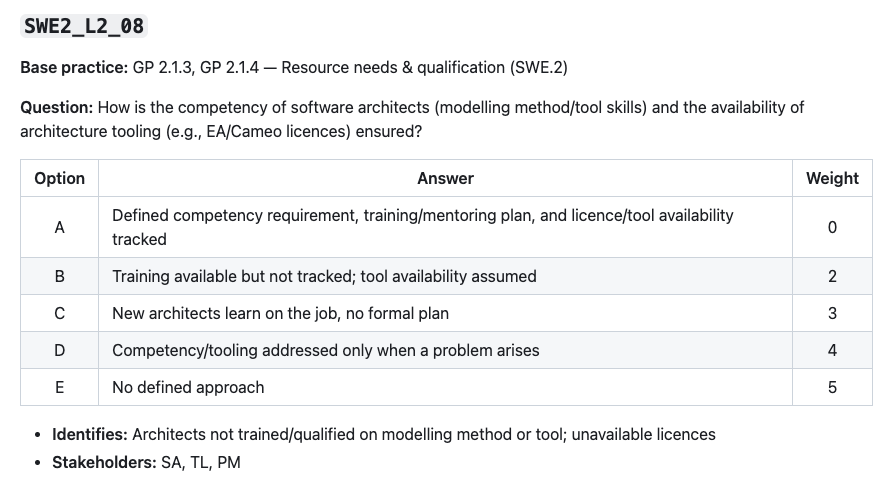
\includegraphics[width=0.95\textwidth,height=0.3\textheight,keepaspectratio]{src/Q19.png}\\[0.3cm]
  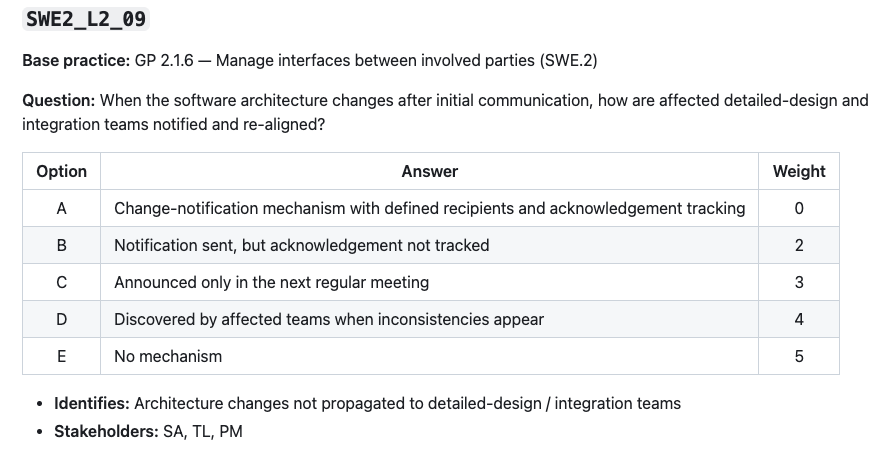
\includegraphics[width=0.95\textwidth,height=0.3\textheight,keepaspectratio]{src/Q20.png}\\[0.3cm]
  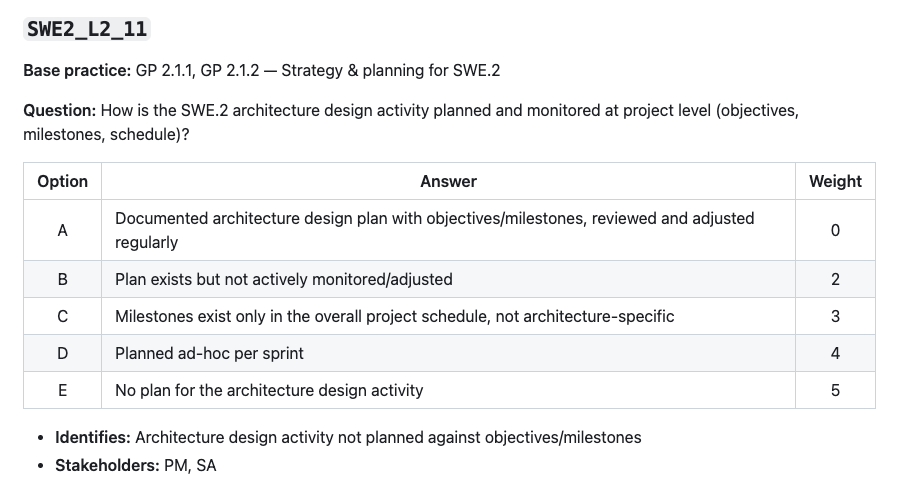
\includegraphics[width=0.95\textwidth,height=0.3\textheight,keepaspectratio]{src/Q21.png}\\[0.3cm]
  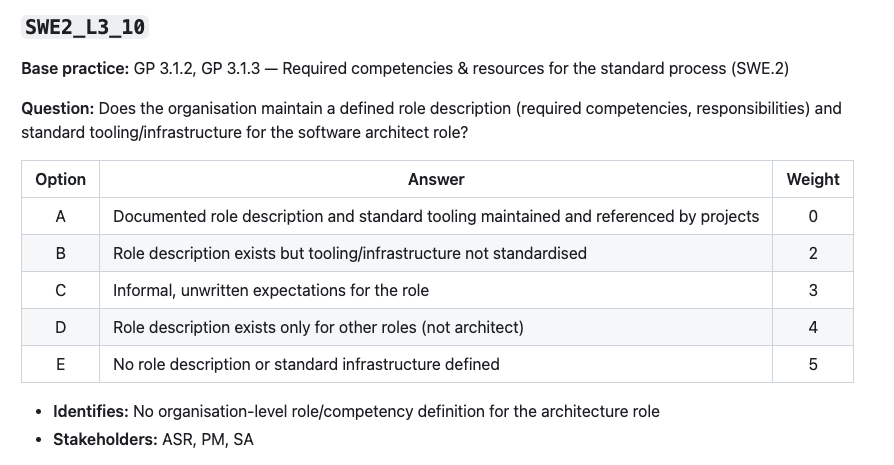
\includegraphics[width=0.95\textwidth,height=0.3\textheight,keepaspectratio]{src/Q22.png}
\end{center}

\section*{SWE.3: Software Detailed Design and Unit Construction}

\begin{center}
  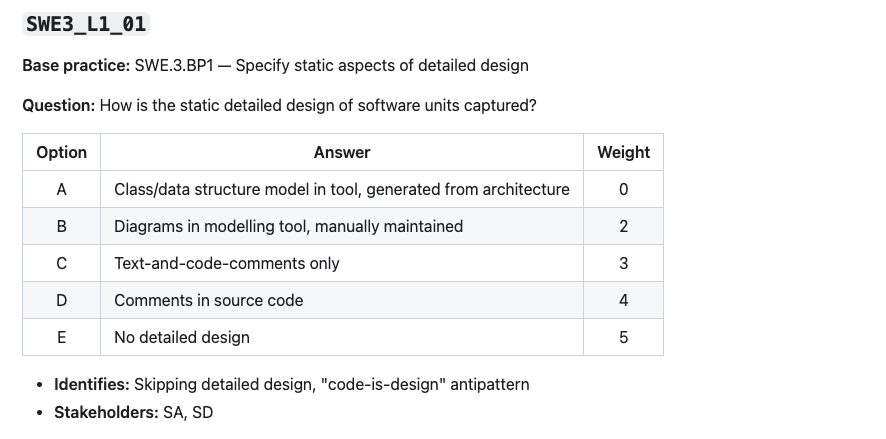
\includegraphics[width=0.95\textwidth,height=0.3\textheight,keepaspectratio]{src/Q23.png}\\[0.3cm]
  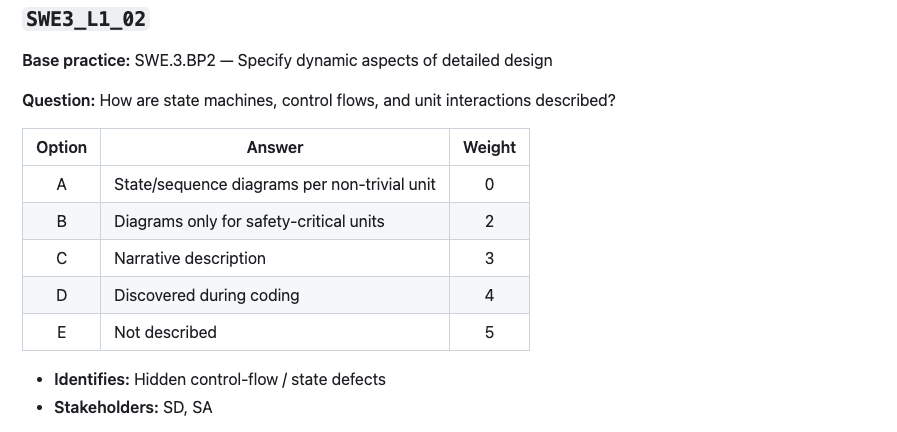
\includegraphics[width=0.95\textwidth,height=0.3\textheight,keepaspectratio]{src/Q24.png}\\[0.3cm]
  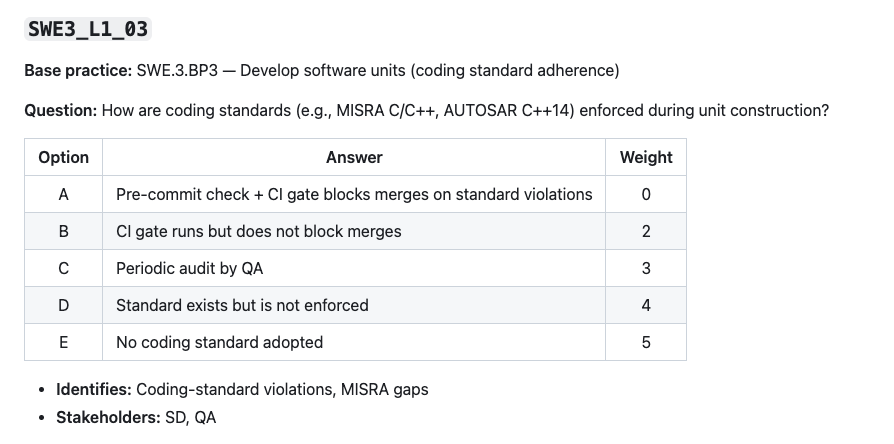
\includegraphics[width=0.95\textwidth,height=0.3\textheight,keepaspectratio]{src/Q25.png}\\[0.3cm]
  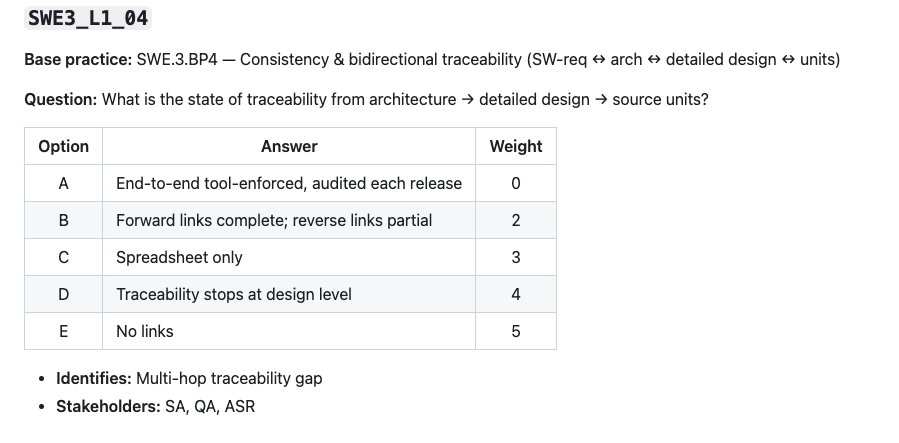
\includegraphics[width=0.95\textwidth,height=0.3\textheight,keepaspectratio]{src/Q26.png}\\[0.3cm]
  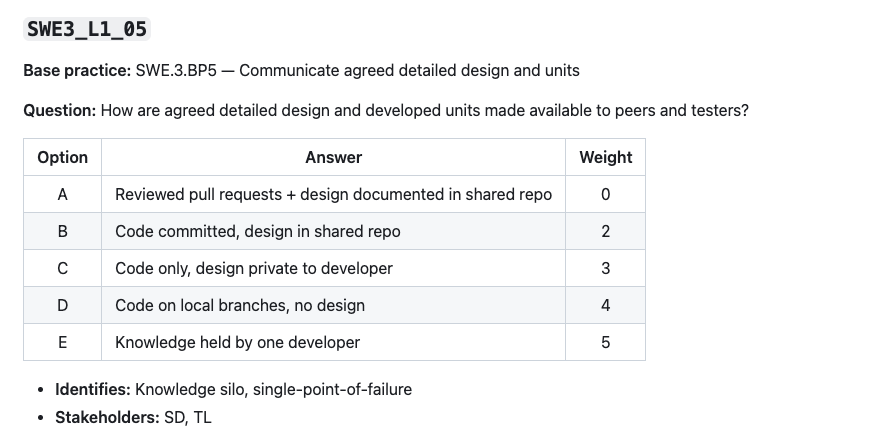
\includegraphics[width=0.95\textwidth,height=0.3\textheight,keepaspectratio]{src/Q27.png}\\[0.3cm]
  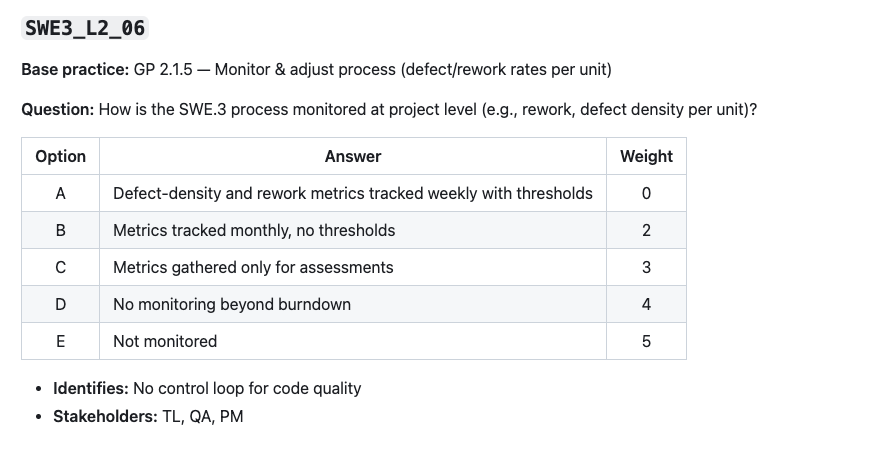
\includegraphics[width=0.95\textwidth,height=0.3\textheight,keepaspectratio]{src/Q28.png}\\[0.3cm]
  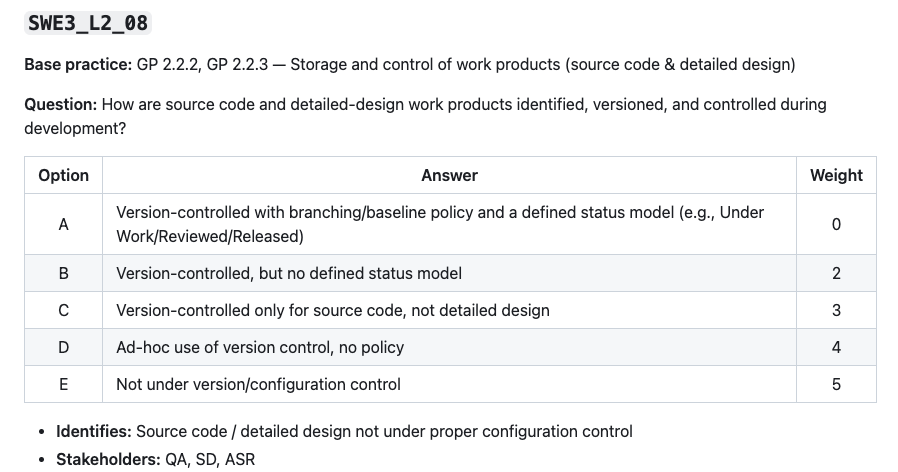
\includegraphics[width=0.95\textwidth,height=0.3\textheight,keepaspectratio]{src/Q29.png}\\[0.3cm]
  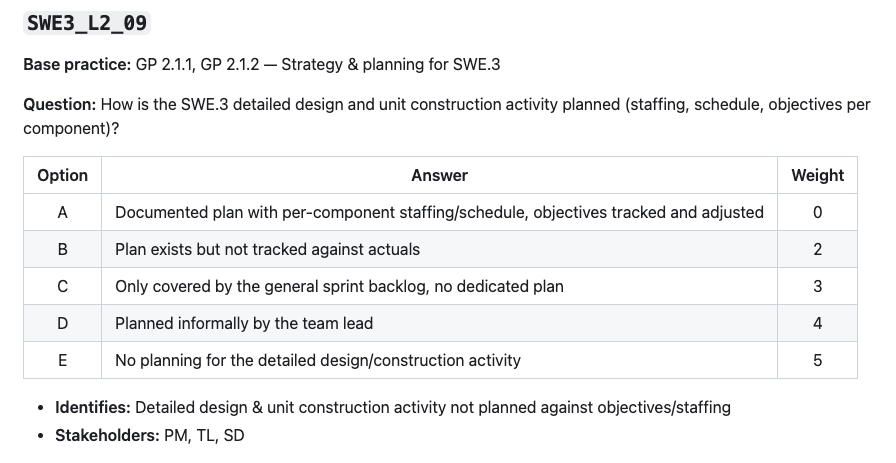
\includegraphics[width=0.95\textwidth,height=0.3\textheight,keepaspectratio]{src/Q30.png}\\[0.3cm]
  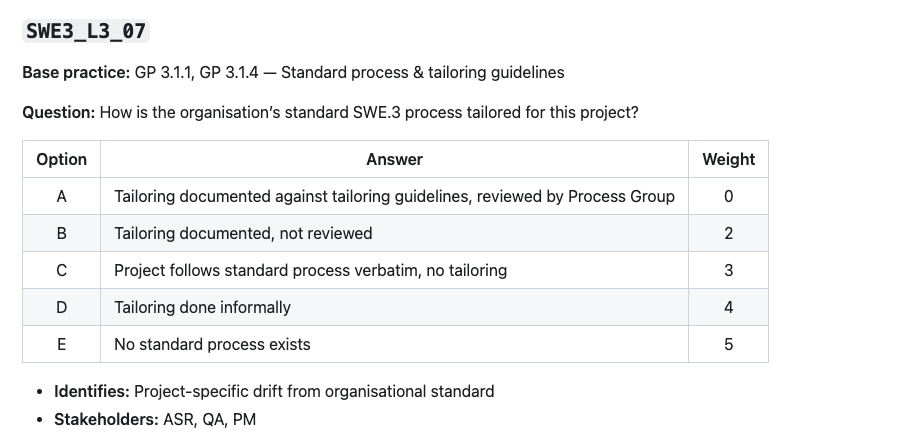
\includegraphics[width=0.95\textwidth,height=0.3\textheight,keepaspectratio]{src/Q31.png}
\end{center}

\section*{SWE.4: Software Unit Verification}

\begin{center}
  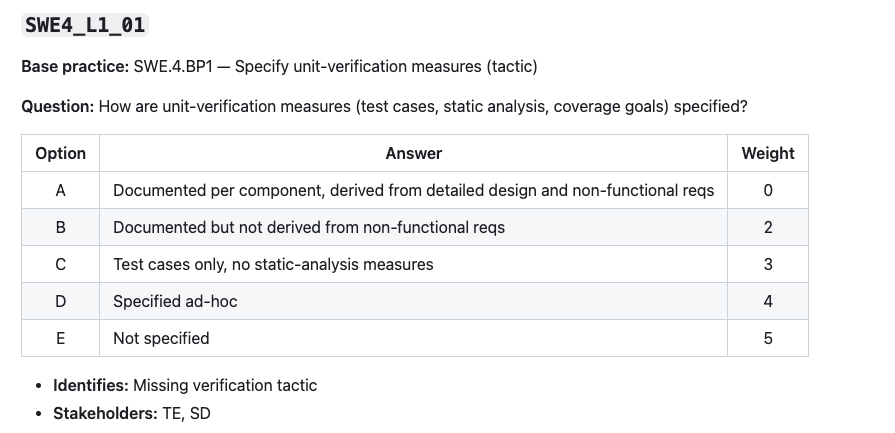
\includegraphics[width=0.95\textwidth,height=0.3\textheight,keepaspectratio]{src/Q32.png}\\[0.3cm]
  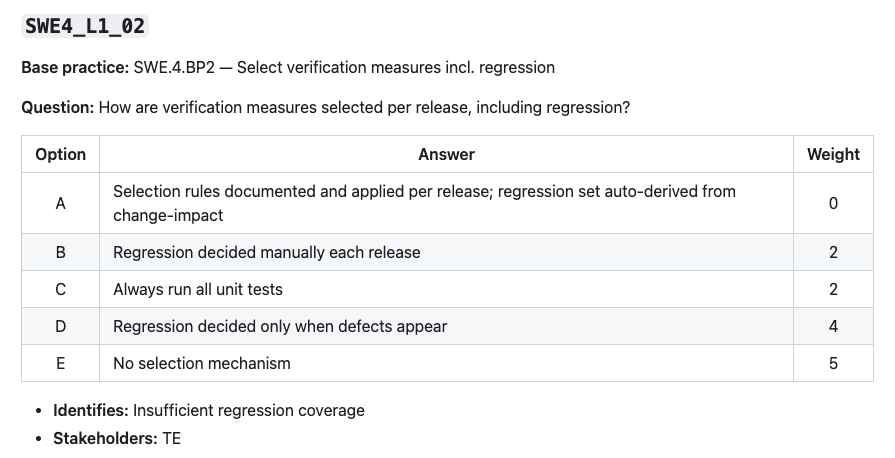
\includegraphics[width=0.95\textwidth,height=0.3\textheight,keepaspectratio]{src/Q33.png}\\[0.3cm]
  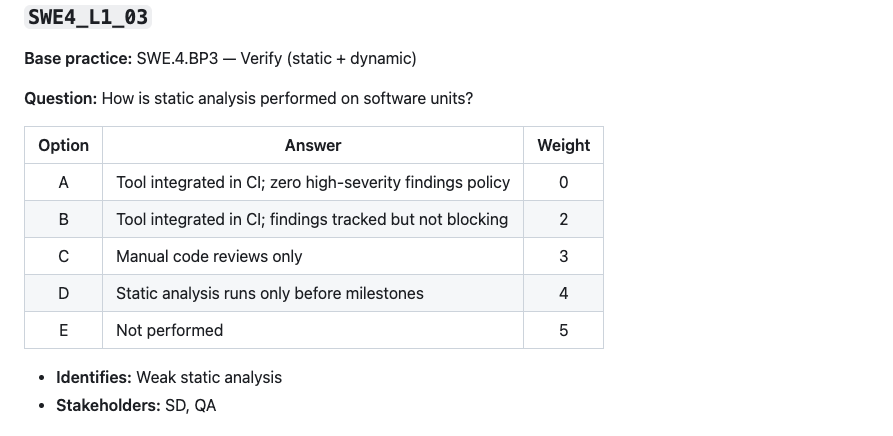
\includegraphics[width=0.95\textwidth,height=0.3\textheight,keepaspectratio]{src/Q34.png}\\[0.3cm]
  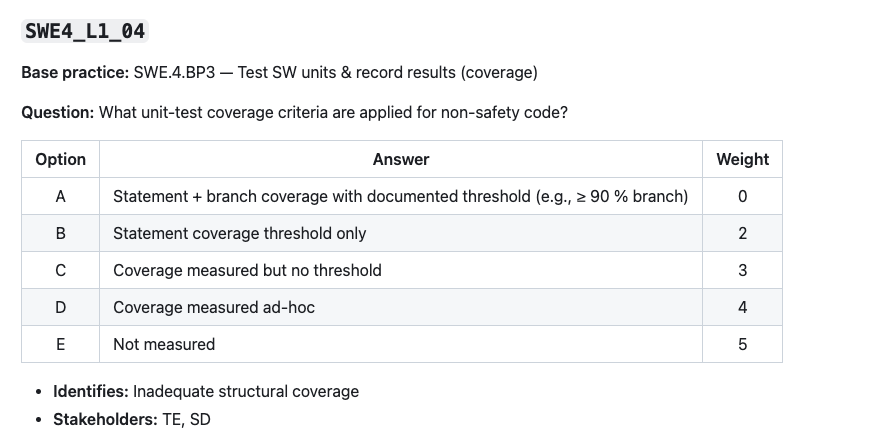
\includegraphics[width=0.95\textwidth,height=0.3\textheight,keepaspectratio]{src/Q35.png}\\[0.3cm]
  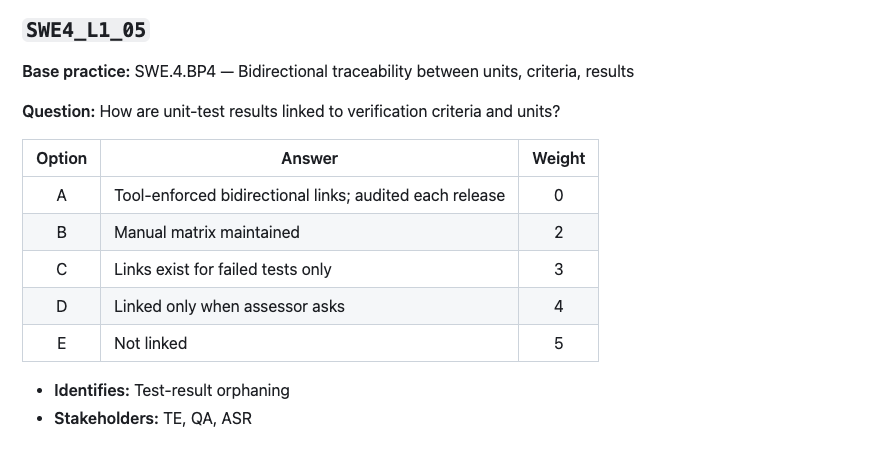
\includegraphics[width=0.95\textwidth,height=0.3\textheight,keepaspectratio]{src/Q36.png}\\[0.3cm]
  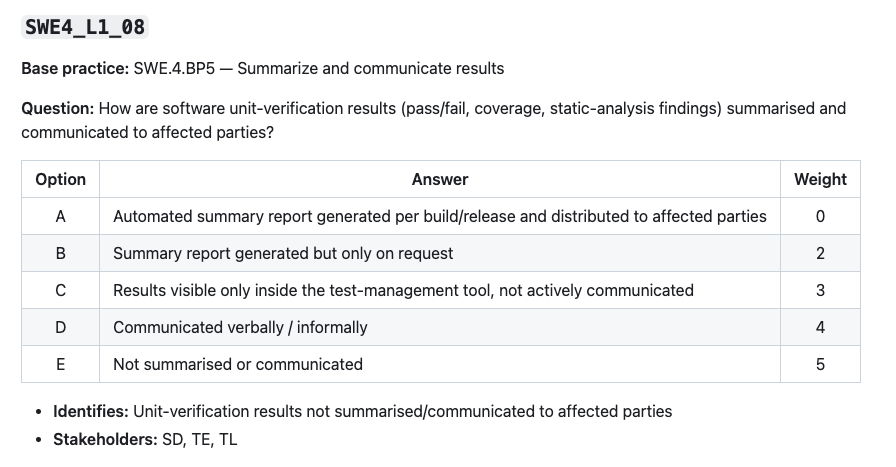
\includegraphics[width=0.95\textwidth,height=0.3\textheight,keepaspectratio]{src/Q37.png}\\[0.3cm]
  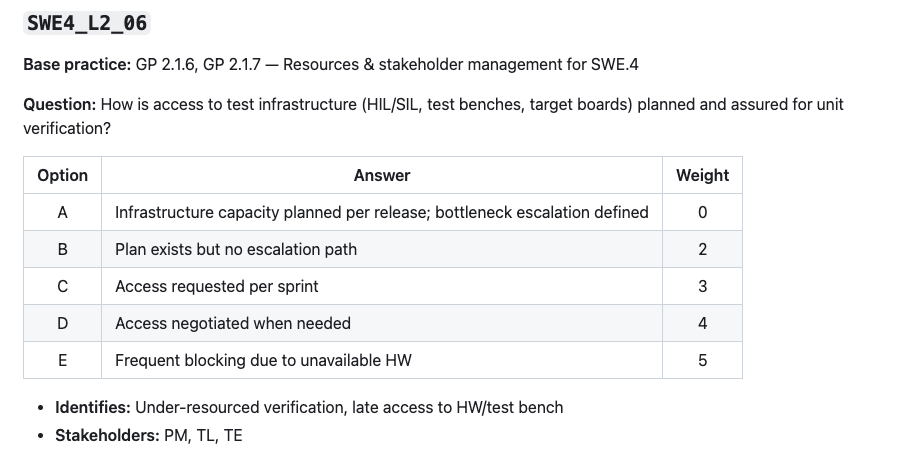
\includegraphics[width=0.95\textwidth,height=0.3\textheight,keepaspectratio]{src/Q38.png}\\[0.3cm]
  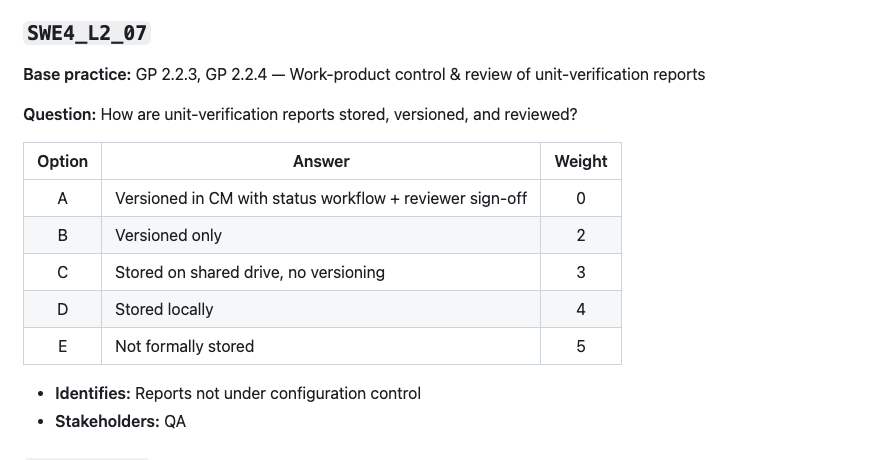
\includegraphics[width=0.95\textwidth,height=0.3\textheight,keepaspectratio]{src/Q39.png}\\[0.3cm]
  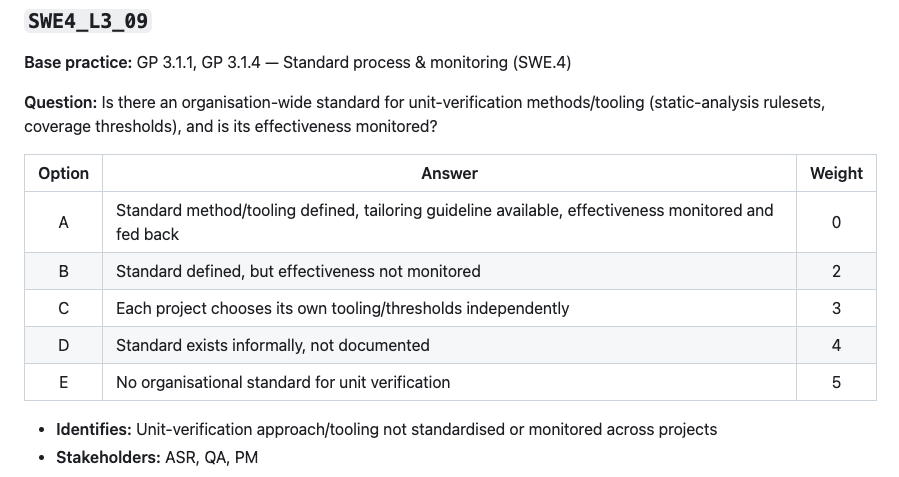
\includegraphics[width=0.95\textwidth,height=0.3\textheight,keepaspectratio]{src/Q40.png}
\end{center}

\section*{SWE.5: Software Component Verification and Integration Verification}

\begin{center}
  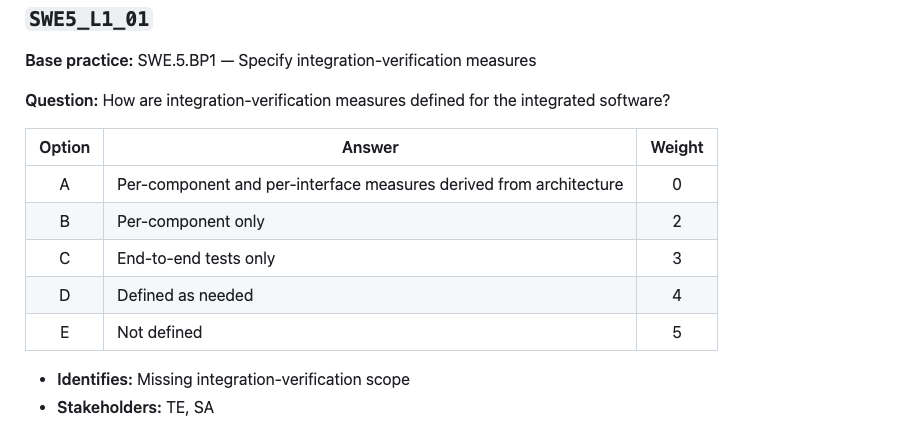
\includegraphics[width=0.95\textwidth,height=0.3\textheight,keepaspectratio]{src/Q41.png}\\[0.3cm]
  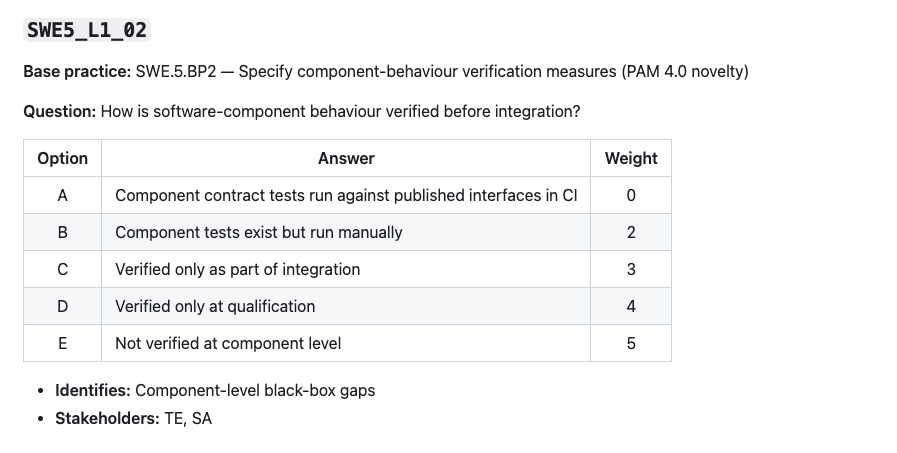
\includegraphics[width=0.95\textwidth,height=0.3\textheight,keepaspectratio]{src/Q42.png}\\[0.3cm]
  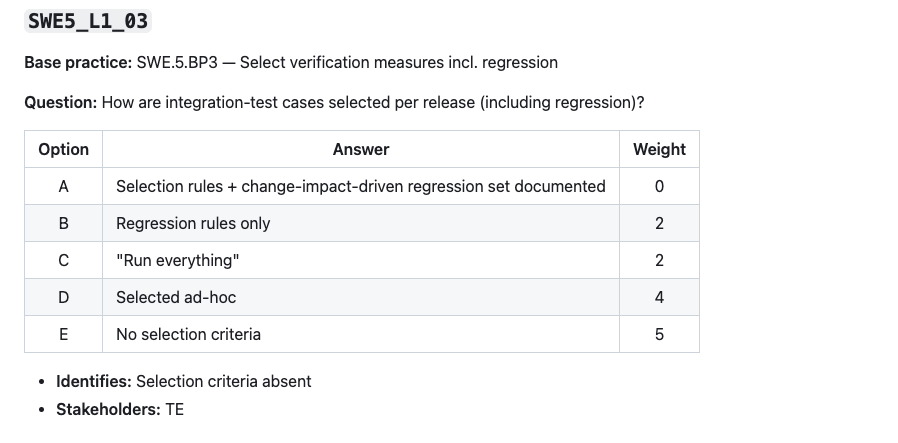
\includegraphics[width=0.95\textwidth,height=0.3\textheight,keepaspectratio]{src/Q43.png}\\[0.3cm]
  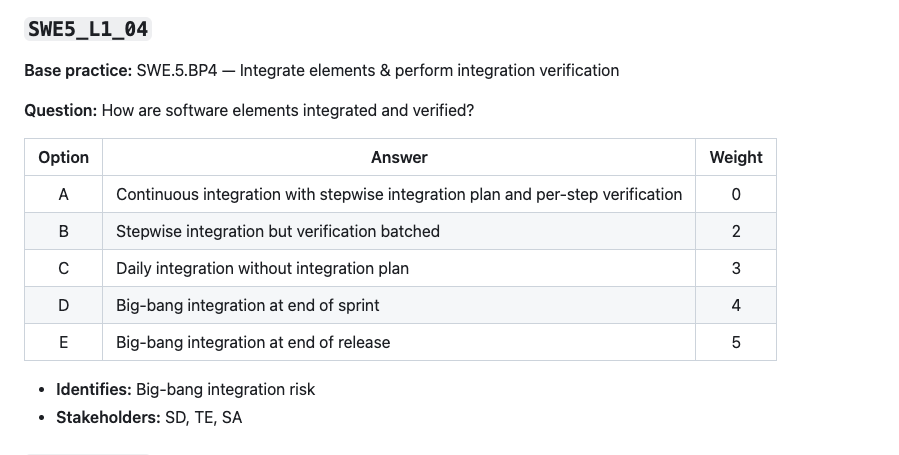
\includegraphics[width=0.95\textwidth,height=0.3\textheight,keepaspectratio]{src/Q44.png}\\[0.3cm]
  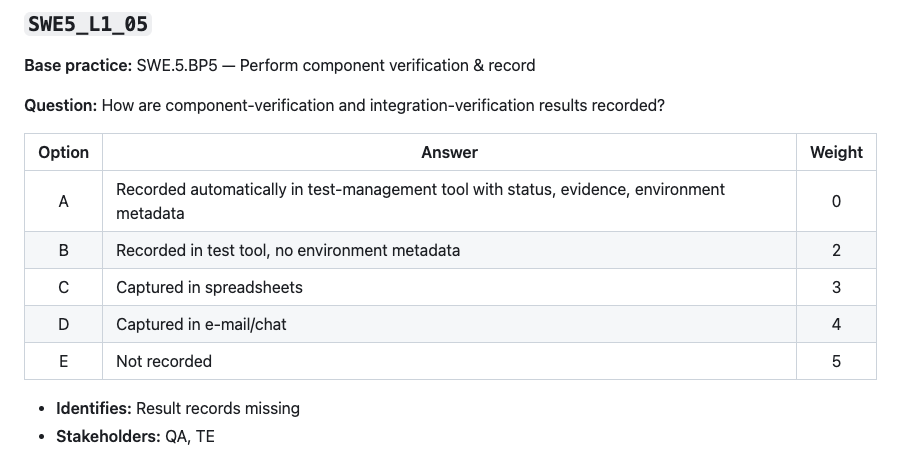
\includegraphics[width=0.95\textwidth,height=0.3\textheight,keepaspectratio]{src/Q45.png}\\[0.3cm]
  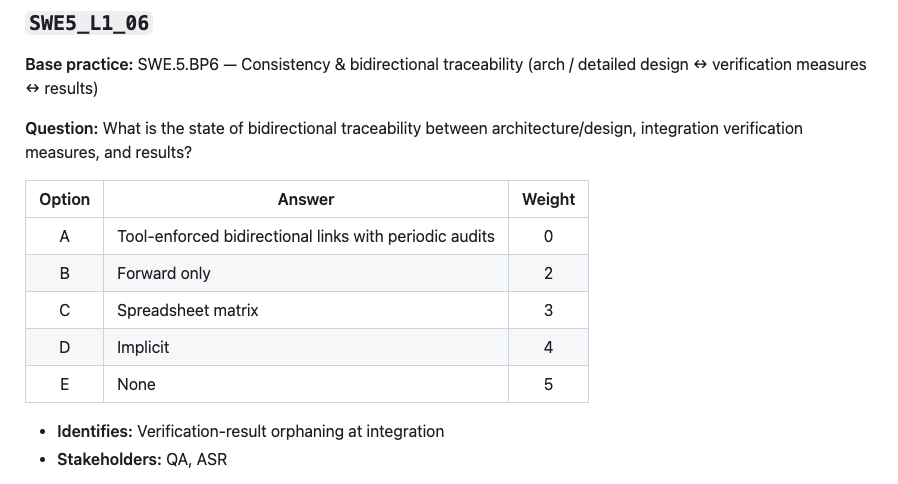
\includegraphics[width=0.95\textwidth,height=0.3\textheight,keepaspectratio]{src/Q46.png}\\[0.3cm]
  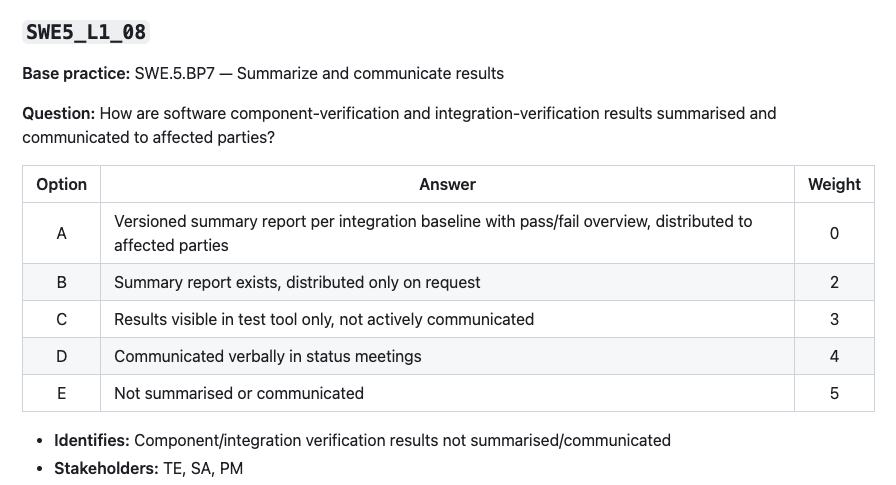
\includegraphics[width=0.95\textwidth,height=0.3\textheight,keepaspectratio]{src/Q47.png}\\[0.3cm]
  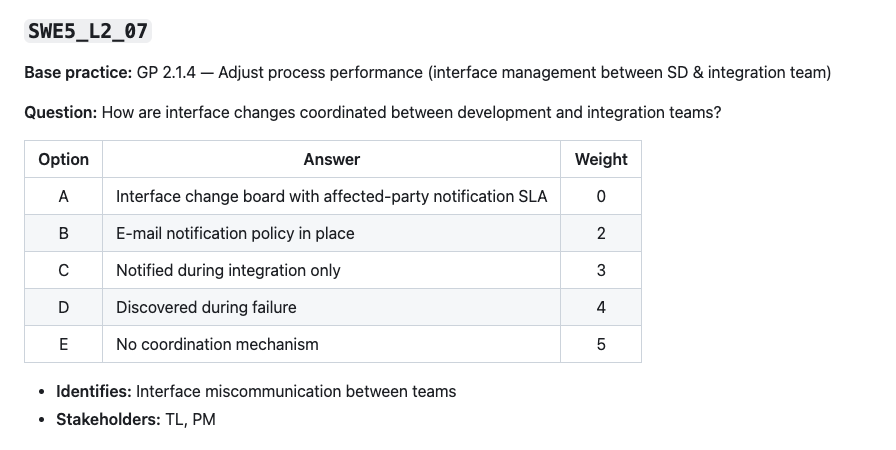
\includegraphics[width=0.95\textwidth,height=0.3\textheight,keepaspectratio]{src/Q48.png}\\[0.3cm]
  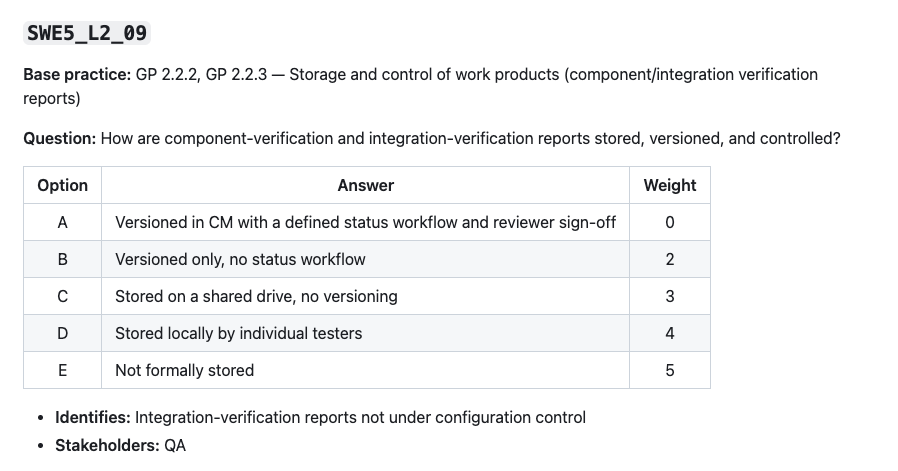
\includegraphics[width=0.95\textwidth,height=0.3\textheight,keepaspectratio]{src/Q49.png}\\[0.3cm]
  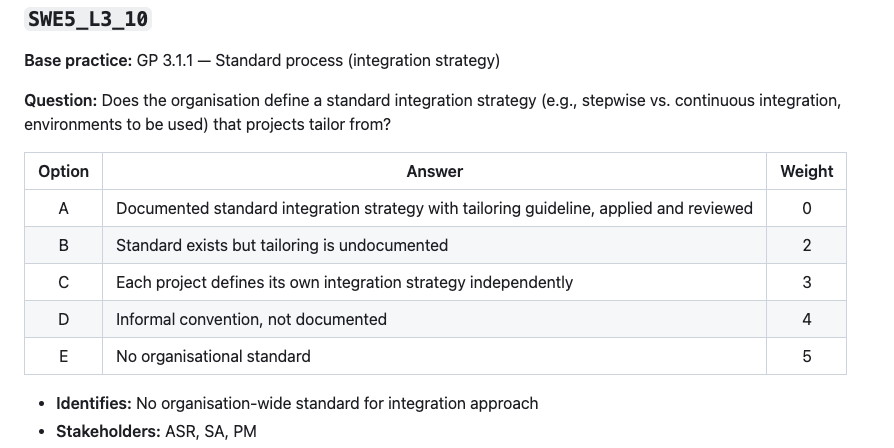
\includegraphics[width=0.95\textwidth,height=0.3\textheight,keepaspectratio]{src/Q50.png}
\end{center}

\section*{SWE.6: Software Verification}

\begin{center}
  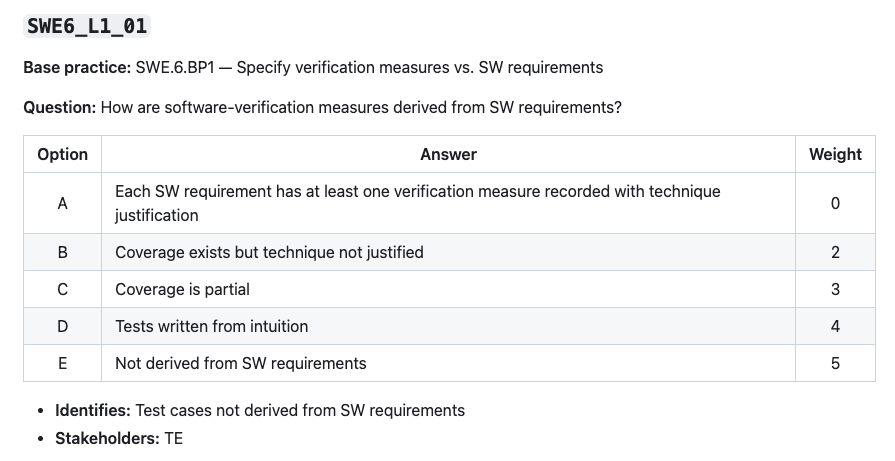
\includegraphics[width=0.95\textwidth,height=0.3\textheight,keepaspectratio]{src/Q51.png}\\[0.3cm]
  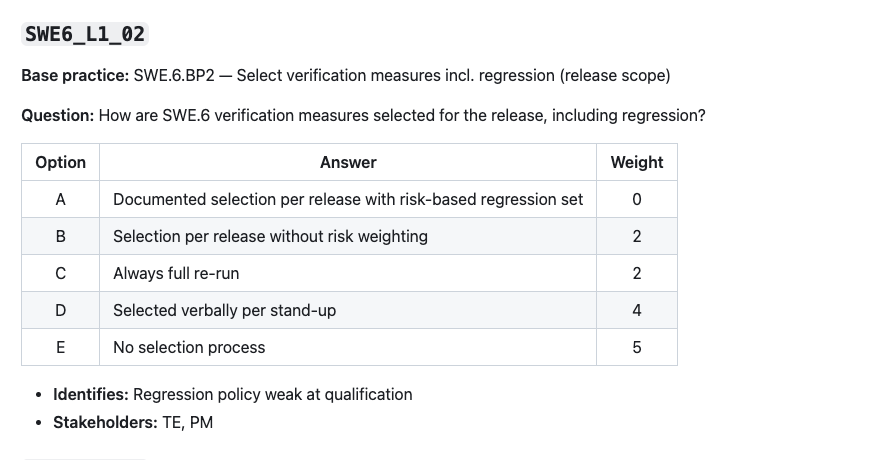
\includegraphics[width=0.95\textwidth,height=0.3\textheight,keepaspectratio]{src/Q52.png}\\[0.3cm]
  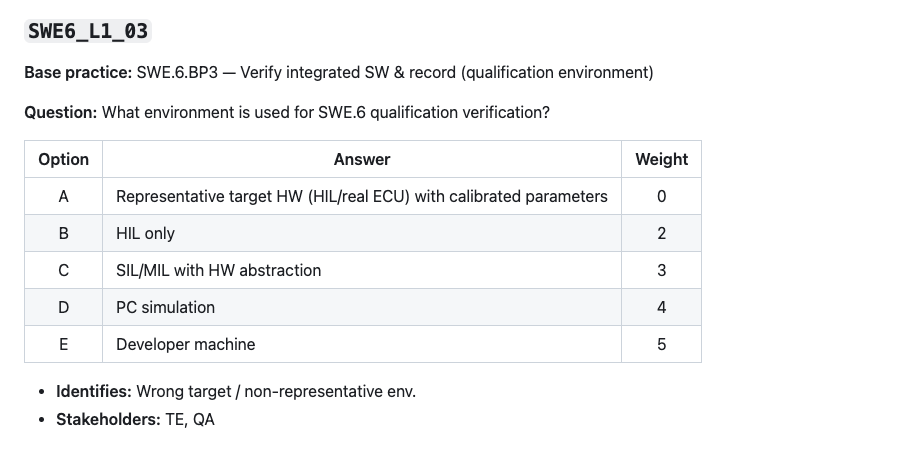
\includegraphics[width=0.95\textwidth,height=0.3\textheight,keepaspectratio]{src/Q53.png}\\[0.3cm]
  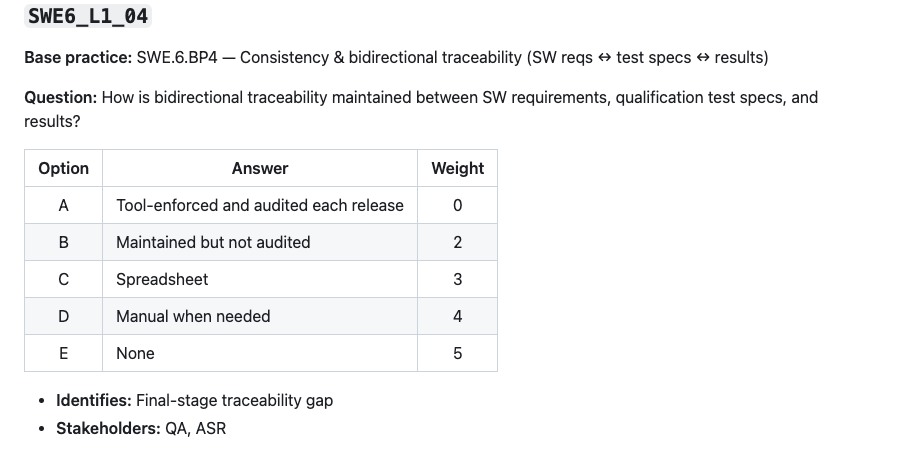
\includegraphics[width=0.95\textwidth,height=0.3\textheight,keepaspectratio]{src/Q54.png}\\[0.3cm]
  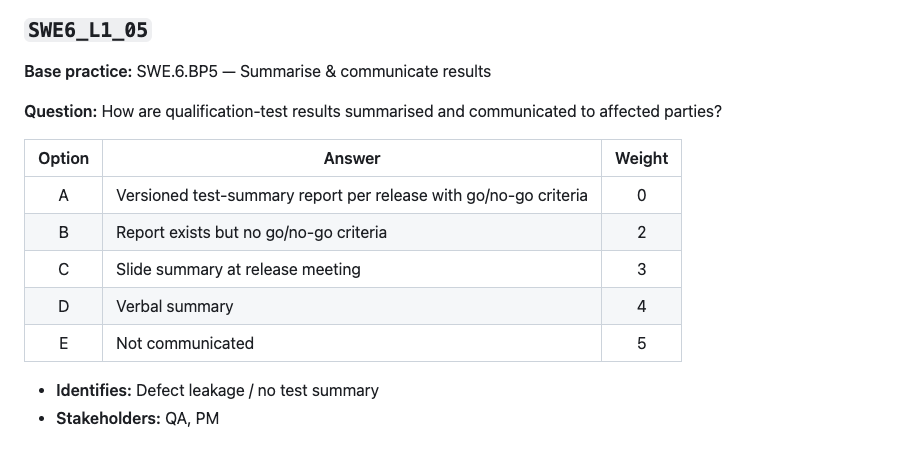
\includegraphics[width=0.95\textwidth,height=0.3\textheight,keepaspectratio]{src/Q55.png}\\[0.3cm]
  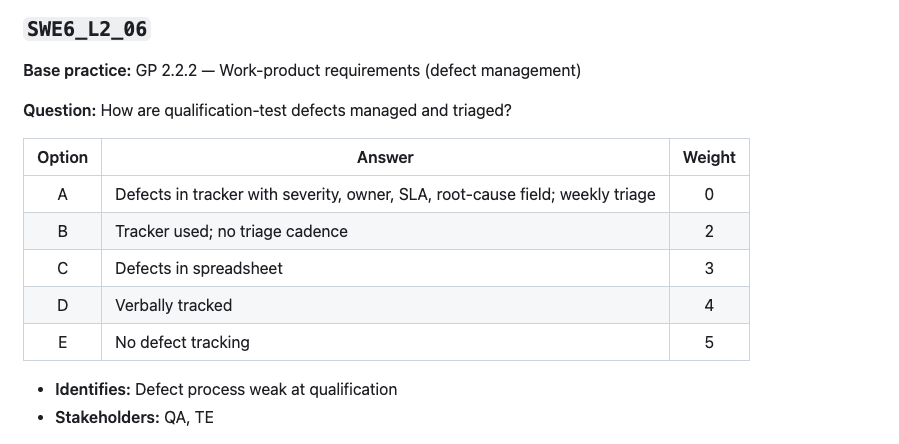
\includegraphics[width=0.95\textwidth,height=0.3\textheight,keepaspectratio]{src/Q56.png}\\[0.3cm]
  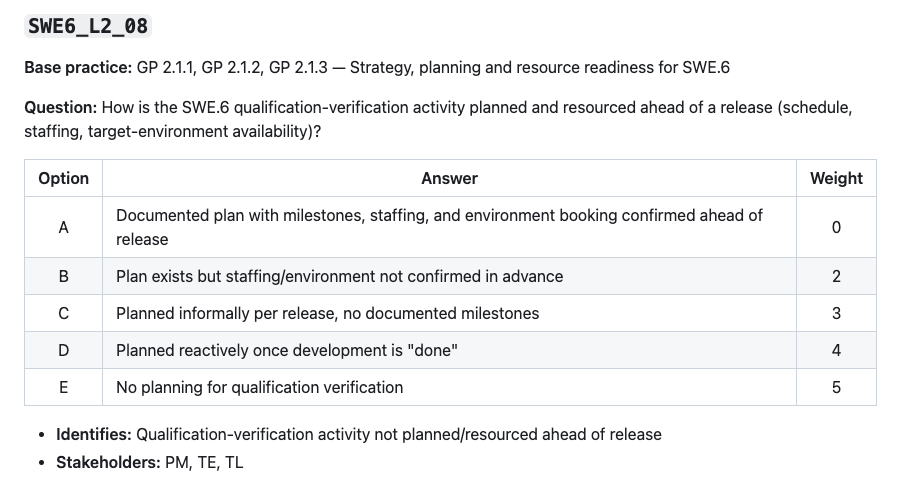
\includegraphics[width=0.95\textwidth,height=0.3\textheight,keepaspectratio]{src/Q57.png}\\[0.3cm]
  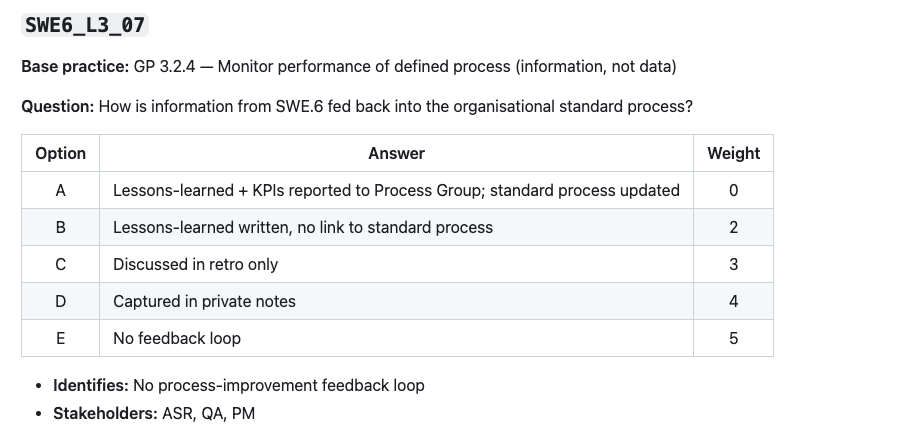
\includegraphics[width=0.95\textwidth,height=0.3\textheight,keepaspectratio]{src/Q58.png}\\[0.3cm]
  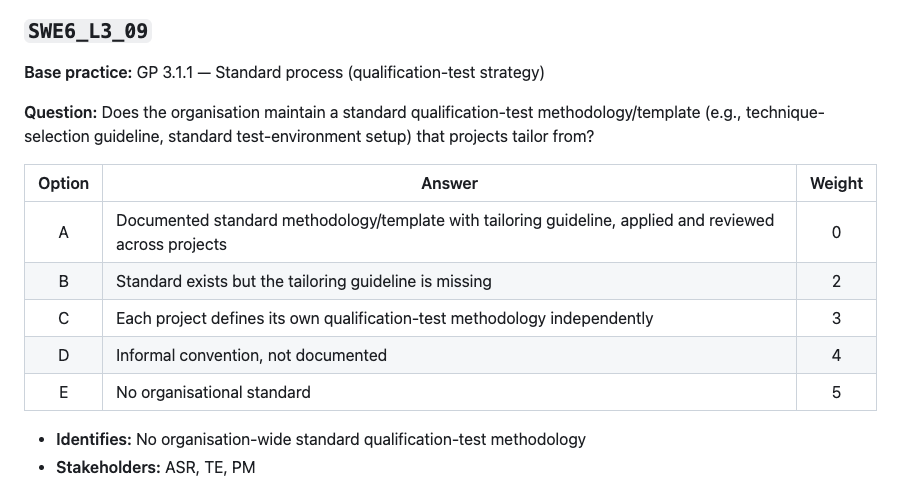
\includegraphics[width=0.95\textwidth,height=0.3\textheight,keepaspectratio]{src/Q59.png}
\end{center}

\printindex

\end{document}
